\documentclass[fleqn,10pt]{report}
%\documentclass[twoside]{report}
\usepackage[a4paper, margin=1.1in]{geometry}
\usepackage{amssymb,amsmath}
\usepackage{mathpartir}
\usepackage{listings}
\usepackage{lstlhs}
\usepackage{doc/saoithin}
\usepackage{tikz}
\usepackage{tikz-cd}
\usetikzlibrary{arrows,matrix}
\usepackage{graphicx}
\usepackage{epstopdf}

\def\includepicture#1{\includegraphics{#1.eps}}

\parindent=0pt % I hate first line indentation
\parskip=3pt   % I like a visual white gap between paragraphs


\author{
  Andrew Butterfield%
  ,\\Andrew Anderson%
  , Colm~Bhandal%
  , Simon~Dardis%
  ,\\Ian~Fitzpatrick%
  , Karen~Forde%
  , Luke~McGuinness%
  }
\title{\UTP2
  \\{\normalsize
      Unifying Theories of Programming Theorem-Prover
  \\  (a.k.a. \Saoithin)}
}

\def\TODO#1{%
  \textbf{ToDo: }
  \textit{#1}
}

%
% This document provides a single place for definitions
% that will appear in multiple locations,
% and so ensures they are kept consistent.
%
% This does not generate any typeset output.
%
\def\DEFOEESUBST{
  \begin{eqnarray*}
     k[\vec x:=\vec e] &\defs& k
  \\ x[\vec x:=\vec e]
     &\defs& \left\{
               \begin{array}{ll}
                 e_i, & i \mbox{ exists, s.t.: }x=x_i \\
                 x, & x \notin \vec x
               \end{array}
             \right.
  \\ (f~e)[\vec x:=\vec e] &\defs& f~(e[\vec x:=\vec e])
  \\ E[\vec x:=\vec e] &\defs&
     \left\{
     \begin{array}{ll}
       E[\vec e/\vec x], & E \mbox{ not $\Lambda$-bound higher up} \\
       E, & E \mbox{ is $\Lambda$-bound higher up}
     \end{array}
   \right.
  \\ (\lambda \vec y, \lstvec q @ e)[\vec x:=\vec e]
     &\defs& \lambda \vec y,\lstvec q @ (e[\vec x:=\vec e]\hide\vec y)
  \\ (\Lambda \vec E @ e)[\vec x:=\vec e] &\defs& \Lambda \vec E @ (e[\vec x:=\vec e])
  \\ (\Lambda \vec P @ e)[\vec x:=\vec e] &\defs& \Lambda \vec P @ (e[\vec x:=\vec e])
  \\ (e[\vec f/\vec y])[\vec x:=\vec e] &\defs& e([\vec f/\vec y][\vec e/\vec x])
  \\ (e[\vec e/\vec E])[\vec x:=\vec e] &\defs& \mbox{need to do inner subst first}
  \\ (e[\vec p/\vec P])[\vec x:=\vec e] &\defs& \mbox{need to do inner subst first}
  \\ (e = e)[\vec x:=\vec e] &\defs& e[\vec x:=\vec e] = e[\vec x:=\vec e]
  \\ (\theta x | P @ Q)[\vec x:=\vec e] &\defs& \theta x | P[\vec x:=\vec e]\hide x @ Q[\vec x:=\vec e]\hide x
  \end{eqnarray*}
}

\def\DEFOEPSUBST#1{
\begin{array}{rcl@{$\quad$}l}
   True[\vec x:=\vec e] &\defs&  True
\\ False[\vec x:=\vec e] &\defs& False
\\  e[\vec x:=\vec e] &\defs& \mbox{see Figure \ref{#1}}
\\  (e:t)[\vec x:=\vec e] &\defs& (e[\vec x:=\vec e]:t)
\\  (\mathcal D~e)[\vec x:=\vec e] &\defs& \mathcal D~(e[\vec x:=\vec e])
\\ (\lnot p)[\vec x:=\vec e] &\defs& \lnot (p[\vec x:=\vec e])
\\ (p~ \maltese q)[\vec x:=\vec e] &\defs& p[\vec x:=\vec e]~ \maltese q[\vec x:=\vec e]
\\ P[\vec x:=\vec e] &\defs&
   \left\{
     \begin{array}{ll}
       P[\vec e/\vec x], & P \mbox{ not $\Lambda$-bound higher up} \\
       P, & P \mbox{ is $\Lambda$-bound higher up}
     \end{array}
   \right.
\\ (\yen \vec y,\lstvec q | p @ q)[\vec x:=\vec e]
   &\defs& \yen \vec y,\lstvec q | (p[\vec x:=\vec e]\hide \vec y) @ (q[\vec x:=\vec e]\hide \vec y))
\\ (\yen \vec P @ p)[\vec x:=\vec e] &\defs& \yen \vec P @ (p[\vec x:=\vec e])
\\ (\yen \vec E @ p)[\vec x:=\vec e] &\defs& \yen \vec E @ (p[\vec x:=\vec e])
\\ {}[ p ][\vec x:=\vec e] &\defs& {}[p]
\\ (\Lambda \vec y,\lstvec q @ p)[\vec x:=\vec e]
   &\defs& \Lambda \vec y,\lstvec q @ (p[\vec x:=\vec e]\hide \vec y)
\\ (\Lambda \vec P @ p)[\vec x:=\vec e] &\defs& \Lambda \vec P @ (p[\vec x:=\vec e])
\\ (p~\lstvec q)[\vec x:=\vec e] &\defs& (p[\vec x:=\vec e] ~\lstvec q[\vec x:=\vec e] )
\\ (p~\vec f)[\vec x:=\vec e] &\defs& (p[\vec x:=\vec e]~\vec f[\vec x:=\vec e])
\\ (p[\vec f/\vec y])[\vec x:=\vec e] &\defs& p([\vec f/\vec y][\vec e/\vec x])
\\ (p[\vec e/\vec E])[\vec x:=\vec e] &\defs& \mbox{need to do inner subst first}
\\ (p[\vec p/\vec P])[\vec x:=\vec e] &\defs& \mbox{need to do inner subst first}
\\ (p~S)[\vec x:=\vec e] &\defs& p[\vec x:=\vec e]~S[\vec x:=\vec e]
\\ (p \in S)[\vec x:=\vec e] &\defs& p[\vec x:=\vec e] \in S[\vec x:=\vec e]
\\
\\ S[\vec x:=\vec e] &\defs& S[\vec e/\vec x]
\\ \{ \vec p \}[\vec x:=\vec e] &\defs& \{ \vec p[\vec x:=\vec e] \}
\\ \{ \vec P | r @ p \}[\vec x:=\vec e]
    &\defs& \{ \vec P | r[\vec x:=\vec e] @ p[\vec x:=\vec e] \}
\\ (ps_1 \bigcup ps_2)[\vec x:=\vec e] &\defs& ps_1[\vec x:=\vec e] \bigcup ps_2[\vec x:=\vec e]
\end{array}
}

\def\DEFEEESUBST{
  \begin{eqnarray*}
     k[\vec E:=\vec e] &\defs& k
  \\ x[\vec E:=\vec e] &\defs& x
    \\ (f~e)[\vec E:=\vec e] &\defs& f~(e[\vec E:=\vec e])
  \\ E[\vec E:=\vec e]
     &\defs& \left\{
               \begin{array}{ll}
                 e_i, & i \mbox{ exists, s.t.: }E=E_i \\
                 E, & E \notin \vec E
               \end{array}
             \right.
  \\ (\lambda \vec x, \lstvec q @ e)[\vec E:=\vec e]
     &\defs& \lambda \vec x,\lstvec q @ (e[\vec E:=\vec e])
  \\ (\Lambda \vec F @ e)[\vec E:=\vec e]
     &\defs& \Lambda \vec F @ (e[\vec E:=\vec e]\hide \vec F)
  \\ (\Lambda \vec P @ e)[\vec E:=\vec e] &\defs& \Lambda \vec P @ (e[\vec E:=\vec e])
  \\ (e[\vec e/\vec x])[\vec E:=\vec e] &\defs& \mbox{need to do inner subst first}
  \\ (e[\vec f\vec F])[\vec E:=\vec e] &\defs& e([\vec f/\vec F][\vec e/\vec E])
  \\ (e[\vec p/\vec P])[\vec E:=\vec e] &\defs& \mbox{need to do inner subst first}
  \\ (e = e)[\vec E:=\vec e] &\defs& e[\vec E:=\vec e] = e[\vec E:=\vec e]
  \\ (\theta x | P @ Q)[\vec E:=\vec e]
     &\defs& \theta x | P[\vec E:=\vec e] @ Q[\vec E:=\vec e]
  \end{eqnarray*}
}

\def\DEFPPESUBST{
  \begin{eqnarray*}
     k[\vec P:=\vec p] &\defs& k
  \\ x[\vec P:=\vec p] &\defs& x
    \\ (f~e)[\vec P:=\vec p] &\defs& f~(e[\vec P:=\vec p])
  \\ E[\vec P:=\vec p] &\defs&
  \left\{
     \begin{array}{ll}
       E[\vec p/\vec P], & E \mbox{ not $\Lambda$-bound higher up} \\
       E, & E \mbox{ is $\Lambda$-bound higher up}
     \end{array}
   \right.
    \\ (\lambda \vec x, \lstvec q @ e)[\vec P:=\vec p]
     &\defs& \lambda \vec x,\lstvec q @ (e[\vec P:=\vec p])
  \\ (\Lambda \vec F @ e)[\vec P:=\vec p]
     &\defs& \Lambda \vec F @ (e[\vec P:=\vec p]\hide \vec F)
  \\ (\Lambda \vec P @ e)[\vec P:=\vec p] &\defs& \Lambda \vec P @ (e[\vec P:=\vec p])
  \\ (e[\vec e/\vec x])[\vec P:=\vec p] &\defs& \mbox{need to do inner subst first}
  \\ (e[\vec e/\vec E])[\vec P:=\vec p] &\defs& \mbox{need to do inner subst first}
  \\ (e[\lstvec q/\vec Q])[\vec P:=\vec p] &\defs& e([\lstvec q/\vec Q][\vec p/\vec P])
  \\ (e = e)[\vec P:=\vec p] &\defs& e[\vec P:=\vec p] = e[\vec P:=\vec p]
  \\ (\theta x | P @ Q)[\vec P:=\vec p]
     &\defs& \theta x | P[\vec P:=\vec p] @ Q[\vec P:=\vec p]
  \end{eqnarray*}
}


\def\DEFEEPSUBST#1{
\begin{array}{rcl@{$\quad$}l}
   True[\vec E:=\vec e] &\defs&  True
\\ False[\vec E:=\vec e] &\defs& False
\\  e[\vec E:=\vec e] &\defs& \mbox{see Figure \ref{#1}}
\\  (e:t)[\vec E:=\vec e] &\defs& (e[\vec E:=\vec e]:t)
\\  (\mathcal D~e)[\vec E:=\vec e] &\defs& \mathcal D~(e[\vec E:=\vec e])
\\ (\lnot p)[\vec E:=\vec e] &\defs& \lnot (p[\vec E:=\vec e])
\\ (p~ \maltese q)[\vec E:=\vec e] &\defs& p[\vec E:=\vec e]~ \maltese q[\vec E:=\vec e]
\\ P[\vec E:=\vec e] &\defs&
   \left\{
     \begin{array}{ll}
       P[\vec e/\vec x], & P \mbox{ not $\Lambda$-bound higher up} \\
       P, & P \mbox{ is $\Lambda$-bound higher up}
     \end{array}
   \right.
\\ (\yen \vec y,\lstvec q | p @ q)[\vec E:=\vec e]
   &\defs& \yen \vec y,\lstvec q | (p[\vec E:=\vec e]) @ (q[\vec E:=\vec e]))
\\ (\yen \vec P @ p)[\vec E:=\vec e] &\defs& \yen \vec P @ (p[\vec E:=\vec e])
\\ (\yen \vec F @ p)[\vec E:=\vec e] &\defs& \yen \vec F @ (p[\vec E:=\vec e]\hide\vec F)
\\ {}[~p~][\vec E:=\vec e] &\defs& {}[~p[\vec E:=\vec e]~]
\\ (\Lambda \vec y,\lstvec q @ p)[\vec E:=\vec e]
   &\defs& \Lambda \vec y,\lstvec q @ (p[\vec E:=\vec e])
\\ (\Lambda \vec P @ p)[\vec E:=\vec e] &\defs& \Lambda \vec P @ (p[\vec E:=\vec e])
\\ (p~\lstvec q)[\vec E:=\vec e] &\defs& (p[\vec E:=\vec e] ~\lstvec q[\vec E:=\vec e] )
\\ (p~\vec f)[\vec E:=\vec e] &\defs& (p[\vec E:=\vec e]~\vec f[\vec E:=\vec e])
\\ (p[\vec f/\vec y])[\vec E:=\vec e] &\defs& \mbox{need to do inner subst first}
\\ (p[\vec e/\vec E])[\vec E:=\vec e] &\defs& p([\vec e/\vec E][\vec e/\vec E]
\\ (p[\vec p/\vec P])[\vec E:=\vec e] &\defs& \mbox{need to do inner subst first}
\\ (p~S)[\vec E:=\vec e] &\defs& p[\vec E:=\vec e]~S[\vec E:=\vec e]
\\ (p \in S)[\vec E:=\vec e] &\defs& p[\vec E:=\vec e] \in S[\vec E:=\vec e]
\\
\\ S[\vec E:=\vec e] &\defs& S[\vec e/\vec E]
\\ \{ \vec p \}[\vec E:=\vec e] &\defs& \{ \vec p[\vec E:=\vec e] \}
\\ \{ \vec P | r @ p \}[\vec E:=\vec e]
    &\defs& \{ \vec P | r[\vec E:=\vec e] @ p[\vec E:=\vec e] \}
\\ (ps_1 \bigcup ps_2)[\vec E:=\vec e] &\defs& ps_1[\vec E:=\vec e] \bigcup ps_2[\vec E:=\vec e]
\end{array}
}

\def\DEFPPPSUBST#1{
\begin{array}{rcl@{$\quad$}l}
   True[\vec P:=\vec p] &\defs&  True
\\ False[\vec P:=\vec p] &\defs& False
\\  e[\vec P:=\vec p] &\defs& \mbox{see Figure \ref{#1}}
\\  (e:t)[\vec P:=\vec p] &\defs& (e[\vec P:=\vec p]:t)
\\  (\mathcal D~e)[\vec P:=\vec p] &\defs& \mathcal D~(e[\vec P:=\vec p])
\\ (\lnot p)[\vec P:=\vec p] &\defs& \lnot (p[\vec P:=\vec p])
\\ (p~ \maltese q)[\vec P:=\vec p] &\defs& p[\vec P:=\vec p]~ \maltese q[\vec P:=\vec p]
\\ P[\vec P:=\vec p] &\defs&
   \left\{
               \begin{array}{ll}
                 p_i, & P \mbox{ not bound higher} \\
                      & \mbox{and exists $i$ s.t.: }P=P_i \\
                 P, & \mbox{otherwise}
               \end{array}
             \right.
\\ (\yen \vec y,\lstvec q | p @ q)[\vec P:=\vec p]
   &\defs& \yen \vec y,\lstvec q | (p[\vec P:=\vec p]) @ (q[\vec P:=\vec p]))
\\ (\yen \vec Q @ p)[\vec P:=\vec p] &\defs& \yen \vec Q @ (p[\vec P:=\vec p]\hide\vec Q)
\\ (\yen \vec F @ p)[\vec P:=\vec p] &\defs& \yen \vec F @ (p[\vec P:=\vec p])
\\ {}[~p~][\vec P:=\vec p] &\defs& {}[~p[\vec P:=\vec p]~]
\\ (\Lambda \vec y,\lstvec q @ p)[\vec P:=\vec p]
   &\defs& \Lambda \vec y,\lstvec q @ (p[\vec P:=\vec p])
\\ (\Lambda \vec Q @ p)[\vec P:=\vec p] &\defs& \Lambda \vec P @ (p[\vec P:=\vec p]\hide \vec Q)
\\ (p~\lstvec q)[\vec P:=\vec p] &\defs& (p[\vec P:=\vec p] ~\lstvec q[\vec P:=\vec p] )
\\ (p~\vec f)[\vec P:=\vec p] &\defs& (p[\vec P:=\vec p]~\vec f[\vec P:=\vec p])
\\ (p[\vec f/\vec y])[\vec P:=\vec p] &\defs& \mbox{need to do inner subst first}
\\ (p[\vec e/\vec E])[\vec P:=\vec p] &\defs& \mbox{need to do inner subst first}
\\ (p[\lstvec q/\vec Q])[\vec P:=\vec p] &\defs& (p([\lstvec q/\vec Q][\vec p/\vec P])
\\ (p~S)[\vec P:=\vec p] &\defs& p[\vec P:=\vec p]~S[\vec P:=\vec p]
\\ (p \in S)[\vec P:=\vec p] &\defs& p[\vec P:=\vec p] \in S[\vec P:=\vec p]
\\
\\ S[\vec P:=\vec p] &\defs& S[\vec p/\vec P]
\\ \{ \vec p \}[\vec P:=\vec p] &\defs& \{ \vec p[\vec P:=\vec p] \}
\\ \{ \vec Q | r @ p \}[\vec P:=\vec p]
    &\defs& \{ \vec P
             | r[\vec P:=\vec p]\hide\vec Q
             @ p[\vec P:=\vec p] \hide\vec Q
            \}
\\ (ps_1 \bigcup ps_2)[\vec P:=\vec p] &\defs& ps_1[\vec P:=\vec p] \bigcup ps_2[\vec P:=\vec p]
\end{array}
}

\def\AXeqvAssocL{(P\equiv Q)\equiv R}
\def\AXeqvAssocR{P\equiv (Q\equiv R)}
\def\AXeqvAssoc{(\AXeqvAssocL) \equiv (\AXeqvAssocR)}
\def\AXeqvAssocN{\LNAME{Ax-$\equiv$-assoc}}

\def\AXeqvSymm{P\equiv Q\equiv Q \equiv P}
\def\AXeqvSymmN{\LNAME{Ax-$\equiv$-symm}}

\def\AXeqvId{\textit{true} \equiv Q\equiv Q}
\def\AXeqvIdN{\LNAME{Ax-$\equiv$-id}}

\def\AXfalseDef{\textit{false} \equiv \neg \mbox{\textit{true}}}
\def\AXfalseDefN{\LNAME{Ax-$false$-def}}

\def\AXnotEqvDistr{\neg(P\equiv Q) \equiv \neg P \equiv Q}
\def\AXnotEqvDistrN{\LNAME{Ax-$\neg$-$\equiv$-distr}}

\def\AXorSymm{P\vee Q \equiv  Q \vee P}
\def\AXorSymmN{\LNAME{Ax-$\vee$-symm}}

\def\AXorAssoc{(P\vee Q) \vee R \equiv  P \vee (Q \vee R)}
\def\AXorAssocN{\LNAME{Ax-$\vee$-assoc}}

\def\AXorIdem{P\vee P \equiv P}
\def\AXorIdemN{\LNAME{Ax-$\vee$-idem}}

\def\AXorEqvDistr{P \vee (Q\equiv R) \equiv P\vee Q \equiv P \vee R}
\def\AXorEqvDistrN{\LNAME{Ax-$\vee$-$\equiv$-distr}}

\def\AXexclMdl{P \vee \neg P}
\def\AXexclMdlN{\LNAME{Ax-Excl-Mdl}}

\def\AXgoldRule{P\wedge Q \equiv  P \equiv Q \equiv P \vee Q}
\def\AXgoldRuleN{\LNAME{Ax-Golden-Rule}}

\def\AXimplDef{P\Rightarrow Q \equiv P\vee  Q \equiv Q}
\def\AXimplDefN{\LNAME{Ax-$\implies$-def}}

\def\AXPROP{
  \begin{array}{ll}
     \AXeqvAssoc & \AXeqvAssocN
  \\ \AXeqvSymm & \AXeqvSymmN
  \\ \AXeqvId & \AXeqvIdN
  \\ \AXfalseDef &\AXfalseDefN
  \\ \AXnotEqvDistr & \AXnotEqvDistrN
  \\ \AXorSymm & \AXorSymmN
  \\ \AXorAssoc & \AXorAssocN
  \\ \AXorIdem & \AXorIdemN
  \\ \AXorEqvDistr & \AXorEqvDistrN
  \\ \AXexclMdl & \AXexclMdlN
  \\ \AXgoldRule & \AXgoldRuleN
  \\ \AXimplDef & \AXimplDefN
  \end{array}
}

\def\AXAllOScopeL{(\forall \lst x,\lst y @ p)}
\def\AXAllOScopeR{(\forall \lst y @ p)}
\def\AXAllOScopeS{\lst x \notin p}
\def\AXAllOScopeN{\LNAME{Ax-$\forall x$-scope}}
\def\AXAllOScope{\AXAllOScopeL \equiv \AXAllOScopeR, \quad \AXAllOScopeS}

\def\AXAllEScopeL{(\forall \lst E, \lst F @ p)}
\def\AXAllEScopeR{(\forall \lst F @ p)}
\def\AXAllEScopeS{\lst E \notin p}
\def\AXAllEScopeN{\LNAME{Ax-$\forall E$-scope}}
\def\AXAllEScope{\AXAllEScopeL \equiv \AXAllEScopeR, \quad \AXAllEScopeS}

\def\AXAllPScopeL{(\forall \lst P,  \lst Q @ p)}
\def\AXAllPScopeR{(\forall \lst Q @ p)}
\def\AXAllPScopeS{ \lst P \notin p}
\def\AXAllPScopeN{\LNAME{Ax-$\forall P$-scope}}
\def\AXAllPScope{\AXAllPScopeL \equiv \AXAllPScopeR, \quad \AXAllPScopeS}


\def\AXorAllOScopeL{p \lor (\forall \lst x,\lst y @ q)}
\def\AXorAllOScopeR{\forall \lst x @ p \lor (\forall \lst y @ q)}
\def\AXorAllOScopeS{\lst x \notin p}
\def\AXorAllOScopeN{\LNAME{Ax-$\lor$-$\forall x$-scope}}
\def\AXorAllOScope{\AXorAllOScopeL \equiv \AXorAllOScopeR, \quad \AXorAllOScopeS}

\def\AXorAllEScopeL{p \lor (\forall \lst E, \lst F @ q)}
\def\AXorAllEScopeR{\forall \lst E @ p \lor (\forall \lst F @ q)}
\def\AXorAllEScopeS{\lst E \notin p}
\def\AXorAllEScopeN{\LNAME{Ax-$\lor$-$\forall E$-scope}}
\def\AXorAllEScope{\AXorAllEScopeL \equiv \AXorAllEScopeR, \quad \AXorAllEScopeS}

\def\AXorAllPScopeL{p \lor (\forall \lst P,  \lst Q @ q)}
\def\AXorAllPScopeR{\forall \lst P @ p \lor (\forall \lst Q @ q)}
\def\AXorAllPScopeS{ \lst P \notin p}
\def\AXorAllPScopeN{\LNAME{Ax-$\lor$-$\forall P$-scope}}
\def\AXorAllPScope{\AXorAllPScopeL \equiv \AXorAllPScopeR, \quad \AXorAllPScopeS}

\def\AXallODistrL{(\forall \lst x @ p \land q)}
\def\AXallODistrR{(\forall \lst x @ p) \land (\forall \lst x @ q)}
\def\AXallODistrN{\LNAME{Ax-$\forall x$-distr}}
\def\AXallODistr{\AXallODistrL \equiv \AXallODistrR}

\def\AXallEDistrL{(\forall \lst E @ p \land q)}
\def\AXallEDistrR{(\forall \lst E @ p) \land (\forall \lst E @ q)}
\def\AXallEDistrN{\LNAME{Ax-$\forall E$-distr}}
\def\AXallEDistr{\AXallEDistrL \equiv \AXallEDistrR}

\def\AXallPDistrL{(\forall \lst P @ p \land q)}
\def\AXallPDistrR{(\forall \lst P @ p) \land (\forall \lst P @ q)}
\def\AXallPDistrN{\LNAME{Ax-$\forall P$-distr}}
\def\AXallPDistr{\AXallPDistrL \equiv \AXallPDistrR}

\def\AXallOInstL{\forall x, \lst x @ p}
\def\AXallOInstR{\forall \lst x  @ p[e/x]}
\def\AXallOInstN{\LNAME{Ax-$\forall x$-inst}}
\def\AXallOInst{(\AXallOInstL) \implies (\AXallOInstR)}

\def\AXallEInstL{\forall E , \lst E @ p}
\def\AXallEInstR{\forall \lst E @ p[e/E]}
\def\AXallEInstN{\LNAME{Ax-$\forall E$-inst}}
\def\AXallEInst{(\AXallEInstL) \implies (\AXallEInstR)}

\def\AXallPInstL{\forall P, \lst P @ q}
\def\AXallPInstR{\forall \lst P @ q[r/P]}
\def\AXallPInstN{\LNAME{Ax-$\forall P$-inst}}
\def\AXallPInst{(\AXallPInstL) \implies (\AXallPInstR)}

\def\AXallORngL{\forall \lst x | r @ p}
\def\AXallORngR{\forall \lst x @ r \implies p}
\def\AXallORngN{\LNAME{Ax-$\forall x$-range}}
\def\AXallORng{(\AXallORngL) \equiv (\AXallORngR)}

\def\AXanyODefL{\exists \lst x @ p}
\def\AXanyODefR{\lnot (\forall \lst x @ \lnot p)}
\def\AXanyODefN{\LNAME{Ax-$\exists x$-def}}
\def\AXanyODef{(\AXanyODefL) \equiv \AXanyODefR}

\def\AXanyEDefL{\exists \lst E @ p}
\def\AXanyEDefR{\lnot (\forall \lst E @ \lnot p)}
\def\AXanyEDefN{\LNAME{Ax-$\exists E$-def}}
\def\AXanyEDef{(\AXanyEDefL) \equiv \AXanyEDefR}

\def\AXanyPDefL{\exists \lst P @ p}
\def\AXanyPDefR{\lnot (\forall \lst P @ \lnot p)}
\def\AXanyPDefN{\LNAME{Ax-$\exists P$-def}}
\def\AXanyPDef{(\AXanyPDefL) \equiv \AXanyPDefR}

\def\AXanyORngL{\exists \lst x | r @ p}
\def\AXanyORngR{\exists \lst x @ r \land p}
\def\AXanyORngN{\LNAME{Ax-$\exists x$-range}}
\def\AXanyORng{(\AXanyORngL) \equiv (\AXanyORngR)}

\def\AXoneODefL{\exists! \lst x @ p}
\def\AXoneODefR{(\exists \lst x @ p)
                 \land
                 \exists \lst y @ p[\lst y/ \lst x] \implies \lst y = \lst x}
\def\AXoneODefN{\LNAME{Ax-$\exists! x$-def}}
\def\AXoneODef{(\AXoneODefL) \equiv (\AXoneODefR)}

\def\AXoneORngL{\exists! \lst x | r @ p}
\def\AXoneORngR{\exists! \lst x @ r \land p}
\def\AXoneORngN{\LNAME{Ax-$\exists! x$-range}}
\def\AXoneORng{(\AXoneORngL) \equiv (\AXoneORngR)}

\def\AXunivClosureL{[p]}
\def\AXunivClosureR{\forall \lst x @ p}
\def\AXunivClosureS{\lst x \supseteq p}
\def\AXunivClosureN{\LNAME{Ax-$[]$-def}}
\def\AXunivClosure{\AXunivClosureL \equiv (\AXunivClosureR), \quad \AXunivClosureS}

\def\AXoneODefL{\exists! \lst x @ p}
\def\AXoneODefR{(\exists \lst x @ p)
                 \land
                 \exists \lst y @ p[\lst y/ \lst x] \implies \lst y = \lst x}
\def\AXoneODefN{\LNAME{Ax-$\exists! x$-def}}
\def\AXoneODef{(\AXoneODefL) \equiv (\AXoneODefR)}

\def\AXeqReflL{e}
\def\AXeqReflR{e}
\def\AXeqReflN{\LNAME{Ax-$=$-refl}}
\def\AXeqRefl{\AXeqReflL = \AXeqReflR}

\def\AXtheDefL{e=\theta x @ p}
\def\AXtheDefR{p[e/x] \land (\forall y @ p[y/x] \implies y=e)}
\def\AXtheDefS{x \notin e}
\def\AXtheDefN{\LNAME{Ax-$\theta$-Def}}
\def\AXtheDef{(\AXtheDefL) \equiv \AXtheDefR, \quad \AXtheDefS}

\def\AXtheRngL{\theta x | r @ p}
\def\AXtheRngR{\theta x @ r \land p}
\def\AXtheRngN{\LNAME{Ax-$\theta$-range}}
\def\AXtheRng{(\AXtheRngL) = (\AXtheRngR)}

\def\AXObetaRedL{(\lambda x, \lst x @ e)f}
\def\AXObetaRedR{(\lambda , \lst x @ e)[f/x]}
\def\AXObetaRedN{\LNAME{Ax-$\beta$-OReduce}}
\def\AXObetaRed{\AXObetaRedL = \AXObetaRedR}

\def\AXEbetaRedL{(\Lambda E, \lst E @ q)e}
\def\AXEbetaRedR{(\Lambda , \lst E @ q)[e/E]}
\def\AXEbetaRedN{\LNAME{Ax-$\beta$-EReduce}}
\def\AXEbetaRed{\AXEbetaRedL \equiv \AXEbetaRedR}

\def\AXPbetaRedL{(\Lambda P, \lst P @ q)r}
\def\AXPbetaRedR{(\Lambda , \lst P @ q)[r/P]}
\def\AXPbetaRedN{\LNAME{Ax-$\beta$-PReduce}}
\def\AXPbetaRed{\AXPbetaRedL \equiv \AXPbetaRedR}

\def\AXLeibnizL{\bigwedge_{i=1}^n x_i = e_i}
\def\AXLeibnizR{p \equiv p[\vec e/\vec x]}
\def\AXLeibnizS{x_i \mbox{ distinct}}
\def\AXLeibnizN{\LNAME{Ax-Leibniz}}
\def\AXLeibniz{(\AXLeibnizL) \implies (\AXLeibnizR), \quad \AXLeibnizS}

\def\AXLLeibnizL{\lst x = \lst e}
\def\AXLLeibnizR{p \equiv p[\lstvec e/\lstvec x]}
\def\AXLLeibnizN{\LNAME{Ax-LLeibniz}}
\def\AXLLeibniz{(\AXLLeibnizL) \implies (\AXLLeibnizR)}

\def\AXOSubstL{p[\vec e/\vec x]}
\def\AXOSubstR{p[\vec x:=\vec e]}
\def\AXOSubstN{\LNAME{Ax-OSubst}}
\def\AXOSubst{\AXOSubstL \equiv \AXOSubstR}

\def\AXESubstL{p[\vec e/\vec E]}
\def\AXESubstR{p[\vec E:=\vec e]}
\def\AXESubstN{\LNAME{Ax-ESubst}}
\def\AXESubst{\AXESubstL \equiv \AXESubstR}

\def\AXPSubstL{p[\vec q/ \vec P]}
\def\AXPSubstR{p[ \vec P:=\vec q]}
\def\AXPSubstN{\LNAME{Ax-PSubst}}
\def\AXPSubst{\AXPSubstL \equiv \AXPSubstR}

\def\AXTrueOSubL{true[\lst e/ \lst x]}
\def\AXTrueOSubR{true}
\def\AXTrueOSubN{\LNAME{Ax-$true$-OSubst}}
\def\AXTrueOSub{\AXTrueOSubL \equiv \AXTrueOSubR}

\def\AXTrueESubL{true[\lst e/ \lst E]}
\def\AXTrueESubR{true}
\def\AXTrueESubN{\LNAME{Ax-$true$-ESubst}}
\def\AXTrueESub{\AXTrueESubL \equiv \AXTrueESubR}

\def\AXTruePSubL{true[\lst q/ \lst P]}
\def\AXTruePSubR{true}
\def\AXTruePSubN{\LNAME{Ax-$true$-PSubst}}
\def\AXTruePSub{\AXTruePSubL \equiv \AXTruePSubR}

\def\AXFalseOSubL{false[\lst e/ \lst x]}
\def\AXFalseOSubR{false}
\def\AXFalseOSubN{\LNAME{Ax-$false$-OSubst}}
\def\AXFalseOSub{\AXFalseOSubL \equiv \AXFalseOSubR}

\def\AXFalseESubL{false[\lst e/ \lst E]}
\def\AXFalseESubR{false}
\def\AXFalseESubN{\LNAME{Ax-$false$-ESubst}}
\def\AXFalseESub{\AXFalseESubL \equiv \AXFalseESubR}

\def\AXFalsePSubL{false[\lst q/ \lst P]}
\def\AXFalsePSubR{false}
\def\AXFalsePSubN{\LNAME{Ax-$false$-PSubst}}
\def\AXFalsePSub{\AXFalsePSubL \equiv \AXFalsePSubR}

\def\AXNONPROP{
  \begin{array}{ll}
     \AXAllOScope & \AXAllOScopeN
  \\ \AXAllEScope & \AXAllEScopeN
  \\ \AXAllPScope & \AXAllPScopeN
  \\
  \\ \AXorAllOScopeL & \AXorAllOScopeN
  \\ {}\equiv (\AXorAllOScopeR), \quad \AXorAllOScopeS
  \\ \AXorAllEScopeL & \AXorAllEScopeN
  \\ {}\equiv (\AXorAllEScopeR), \quad \AXorAllEScopeS
  \\ \AXorAllPScopeL & \AXorAllPScopeN
  \\ {}\equiv (\AXorAllPScopeR), \quad \AXorAllPScopeS
  \\
  \\ \AXallODistr & \AXallODistrN
  \\ \AXallEDistr & \AXallEDistrN
  \\ \AXallPDistr & \AXallPDistrN
  \\
  \\ \AXallOInst & \AXallOInstN
  \\ \AXallEInst & \AXallEInstN
  \\ \AXallPInst & \AXallPInstN
  %\\ \AXallORng  & \AXallORngN
  \\
  \\ \AXanyODef & \AXanyODefN
  \\ \AXanyEDef & \AXanyEDefN
  \\ \AXanyPDef & \AXanyPDefN
  %\\ \AXanyORng & \AXanyORngN
  \\ \AXoneODefL & \AXoneODefN
  \\ {}\equiv \AXoneODefR
  \\ \AXunivClosure & \AXunivClosureN
   %\\ \AXoneORng & \AXoneORngN
  \\
  \\\AXeqRefl & \AXeqReflN
  %
  \\ (\AXtheDefL) & \AXtheDefN
  \\ {} \equiv \AXtheDefR,~\AXtheDefS
  %\\ \AXtheRng & \AXtheRngN
  %
  \\
  \\ \AXObetaRed & \AXObetaRedN
  \\ \AXEbetaRed & \AXEbetaRedN
  \\ \AXPbetaRed & \AXPbetaRedN
  %
  \\
  \\ \AXLeibniz, & \AXLeibnizN
  \\ \AXLeibnizS
  \\
  \\ \AXOSubst & \AXOSubstN
  \\ \AXESubst & \AXESubstN
  \\ \AXPSubst & \AXPSubstN
  \\ \AXTrueOSub & \AXTrueOSubN
  \\ \AXTrueESub & \AXTrueESubN
  \\ \AXTruePSub & \AXTruePSubN
  \\ \AXFalseOSub & \AXFalseOSubN
  \\ \AXFalseESub & \AXFalseESubN
  \\ \AXFalsePSub & \AXFalsePSubN
  \end{array}
}


\def\INFERENCES{
  \begin{array}{ll}
     \INFER{P}{P[Q:=R]}
   & \mbox{(Substitution)}
  \\
  \\ \INFER{P\equiv Q}{R[S:=P] \equiv R[S:=Q]}
   & \mbox{(Leibniz)}
  \\
  \\ \INFER{P, P \equiv Q}{Q}
   & \mbox{(Equanimity)}
  \end{array}
}


\def\DERIVED{
\begin{array}{ll}
   \INFER{P\equiv Q , Q \equiv R}{P \equiv R}
 & \mbox{(Transitivity)}
%
\\ \Gamma \vdash p
   \quad\mbox{iff}\quad
   \Gamma \vdash p \equiv True
 & \mbox{(Truth-is-True)}
%
\\\hline\vspace{-9pt}
\\ \vdash (\forall\vec x,\lstvec q @ True) \equiv True
& \mbox{(Always-True)}
\\ \vdash (\forall \lst E @ True) \equiv True
\\ \vdash (\forall \lst P @ True) \equiv True
%
\\\hline\vspace{-9pt}
\\ \Gamma \vdash p
   \quad\mbox{iff}\quad
    \Gamma \vdash \forall\vec x,\lstvec q @ p
 & \mbox{($\forall$ Intro/Elim)}
\\ \Gamma \vdash p
   \quad\mbox{iff}\quad
    \Gamma \vdash \forall \lst E @ p
\\ \Gamma \vdash p
   \quad\mbox{iff}\quad
    \Gamma \vdash \forall \lst P @ p
%
\\\hline\vspace{-9pt}
\\ p \vdash \forall\vec x,\lstvec q @ p
 & \mbox{(Generalization)}
\\ p \vdash \forall \lst E @ p
 & p \vdash \forall \lst P @ p
%
\\\hline\vspace{-9pt}
\\ p \vdash p[\vec x:=\vec e]
 & \mbox{(Corr. Generalization)}
\\ p \vdash p[\lst E:=\vec e]
 & p \vdash p[ \lst P:=\lstvec q]
%
\\\hline\vspace{-9pt}
\\ \vdash p \implies (\forall\vec x,\vec y,\lstvec q @ r)
 & \mbox{(Universal Consequent 1)}
\\ \quad \equiv
          (\forall\vec x @ p \implies \forall\vec y,\lstvec q @ r),
          \quad \vec x \notin p
\\ \vdash p \implies (\forall \lst E,\lst E @ r)
\\ \quad \equiv
          (\forall \lst E @ p \implies \forall \lst E @ r),
          \quad \lst E \notin p
\\ \vdash p \implies (\forall \lst P, \lst Q @ r)
\\ \quad \equiv
          (\forall \lst P @ p \implies \forall \lst Q @ r),
          \quad  \lst P \notin p
%
\\\hline\vspace{-9pt}
\\ \vdash p \equiv \forall\vec x @ p,
   \quad \vec x \notin p
 & \mbox{(Corr. Univ. Conseq. 1)}
\\ \vdash p \equiv \forall \lst E @ p,
   \quad \lst E \notin p
 & \vdash p \equiv \forall \lst P @ p,
   \quad  \lst P \notin p
%
\\\hline\vspace{-9pt}
\\ \Gamma \vdash p \implies q
   \quad\mbox{iff}\quad
   \Gamma \vdash p \implies \forall\vec x @ q,
   \quad \vec x\notin p
 & \mbox{(Universal Consequent 2)}
\\ \Gamma \vdash p \implies q
   \quad\mbox{iff}\quad
   \Gamma \vdash p \implies \forall \lst E @ q,
   \quad \lst E\notin p
\\ \Gamma \vdash p \implies q
   \quad\mbox{iff}\quad
   \Gamma \vdash p \implies \forall \lst P @ q,
   \quad  \lst P\notin p
%
\\\hline\vspace{-9pt}
\\ \Gamma \vdash q \implies p
   \quad\mbox{iff}\quad
   \Gamma \vdash (\exists \vec x  @ q) \implies p,
   \quad \vec x\notin p
 & \mbox{(Corr. Univ.l Conseq. 2)}
\\ \Gamma \vdash q \implies p
   \quad\mbox{iff}\quad
   \Gamma \vdash (\exists \lst E  @ q) \implies p,
   \quad \lst E\notin p
\\ \Gamma \vdash q \implies p
   \quad\mbox{iff}\quad
   \Gamma \vdash (\exists  \lst P  @ q) \implies p,
   \quad  \lst P\notin p
%
\\\hline\vspace{-9pt}
\\ \vdash (\forall\vec x @ p) \equiv (\forall\vec z @ p[\vec x:=\vec z]),
   \quad \vec z \mbox{ fresh}
 & \mbox{($\alpha$-Renaming)}
\\ \vdash (\forall \lst E @ p) \equiv (\forall \lst F @ p[\lst E:=\lst F]),
   \quad \lst F \mbox{ fresh}
\\ \vdash (\forall \lst P @ p) \equiv (\forall \lst Q @ p[ \lst P:= \lst Q]),
   \quad  \lst Q \mbox{ fresh}
  \end{array}
}

\def\DEDUCTION{
  \begin{array}{ll}
     \Gamma, p \vdash q
     \quad\mbox{then}\quad
     \Gamma \vdash p \implies q,
     \quad p \mbox{ closed}
   & \mbox{(Deduction Theorem)}
  \\ \Gamma \vdash p \implies q
     \quad\mbox{then}\quad
     \Gamma, p \vdash q
   & \mbox{(Deduc. Converse)}
  \\ \Gamma, p[\vec x:=\vec k] \vdash q[\vec x:=\vec k]
     \quad\mbox{then}\quad
     \Gamma \vdash p \implies q,
   & \mbox{(Flexible Deduction)}
  \\\quad \vec x = \fv~p, \vec k \mbox{ constants.}
  \end{array}
}

%
% This document provides a single place for definitions
% that will appear in multiple locations,
% and so ensures they are kept consistent.
%
% This does not generate any typeset output.
%

\def\VARMATHSYNTAX{
\begin{tabular}{lcl@{$\quad$}l}
   $x \in Var$ && (given) & Obs. Variables
\\ $k \in Const$ && (given) & Constants
\\ $f \in FNames$ && (given) & Function Names
\\ $\tau \in TVar$ && (given) & Type Variables
\\ $E \in ENames$ && (given) & Expression Metavariable Names
\\ $P \in PNames$ && (given) & Predicate Metavariable Names
\\ $\lst x,\lst E,\lst P\in LNames$ && (given) & List Variables
\\ $\ell \in QVars_x$        &$::=$& $(x|\lst x)^*_,$
\\ $\varepsilon \in QVars_E$ &$::=$& $(E|\lst E)^*_,$
\\ $\varrho \in QVars_P$     &$::=$& $(P|\lst P)^*_,$
   & Binding Lists
\end{tabular}
}

\def\TYPEMATHSYNTAX{
$$
\begin{array}{lcl@{$\quad$}l}
   t \in Type
 &::=& ? & \mbox{Arbitrary Type}
\\ &|& \litm\Bool & \mbox{Booleans}
\\ &|& \litm\Int & \mbox{Integers}
\\ &|& \tau    & \mbox{Type Variable}
\\ &|& \litm\power~t & \mbox{Sets}
\\ &|& t^+_{\litm \cross} & \mbox{Products}
\\ &|& t^{\litm *} & \mbox{Sequences}
\\ &|& t \litm\fun t & \mbox{Functions}
\\ &|& \litm{Env} & \mbox{Environments }Name \fun Type
\\ &|& \litm{free} & \mbox{Free Types (to be defined)}
\\ &|& \litm\mu ~\tau ~\litm@~ t & \mbox{Recursive Types}
\end{array}
$$
} 

\def\EXPRMATHSYNTAX{
\begin{tabular}{lcl@{$\quad$}l}
   $e \in Expr$ &$::=$& $k$ & Constants
\\              &$|$& $x$  & (Obs.) Variables
\\              &$|$& $f~e$ & Applications
\\              &$|$& $E$ & Expr Metavariable
\\              &$|$& $\litm\lambda~ \ell ~\litm@~ e$ & Obs. Abstraction
\\              &$|$& $e\litm[ e^+_,\litm/x^+_, \litm]$ & Explicit Obs. Substitution
\\              &$|$& $e\litm[ e^+_,\litm/E^+_, \litm]$ & Explicit E-var. Substitution
\\              &$|$& $e\litm[ p^+_,\litm/P^+_, \litm]$ & Explicit P-var. Substitution
\\              &$|$& $e \litm= e$ & Equality
\\              &$|$& $\litm\theta~ x ~[~\litm|~ p~]~ \litm@~ p$  & Definite Description
\end{tabular}
} 
\def\PREDMATHSYNTAX{
\begin{tabular}{lcl@{$\quad$}l}
   $p \in Pred$ &$::=$& $\litm{True} | \litm{False}$ & Constant Predicates
\\              &$|$& $e$ & Atomic Predicate (Boolean-valued Expr.)
\\              &$|$& $e~\litm:~t$ & Type Assertion
\\              &$|$& $\litm{\mathcal D}~e$ & Definedness Assertion.
\\              &$|$& $\litm\lnot p$ & Negation
\\              &$|$& $p~ \maltese q$ & Composites $\maltese \in \setof{\land,\lor,\implies,\equiv,\intchoice,\refinedby}$
\\              &$|$& $P$ & Explicit Metavariable
\\              &$|$& $\yen \ell ~[~\litm|~ p~]~ \litm@ p$ & Observation Quantifiers, $\yen \in \setof{\forall,\exists,\exists!}$
\\              &$|$& $\yen \varrho \litm@ p$ & Predicate Quantifiers,$\yen \in \setof{\mathbf\forall,\mathbf\exists}$
\\              &$|$& $\yen \varepsilon \litm@ p$ & Expression Quantifiers, $\yen \in \setof{\mathbf\forall,\mathbf\exists}$
\\              &$|$& $\litm~[~p~ \litm]$ & Observation Universal Closure
\\              &$|$& $\litm\Lambda~ \varepsilon \litm@ p$ & Expression Abstraction
\\              &$|$& $\litm\Lambda~ \varrho \litm@ p$ & Predicate Abstraction
\\              &$|$& $p~p^+$ & Pred-Pred Application
\\              &$|$& $p~e^+$ & Pred-Expr Application
\\              &$|$& $p\litm[ e^+_,/x^+_, \litm]$ & Explicit Obs. Substitution
\\              &$|$& $p\litm[ e^+_,/E^+_, \litm]$ & Explicit Expr. Substitution
\\              &$|$& $p\litm[ p^+_,/P^+_, \litm]$ & Explicit Pred. Substitution
\\              &$|$& $p~ps$ & Pred-PredSet Application
\\              &$|$& $p ~\litm\in~ ps$ & Predicate Set membership
\\ $ps \in PredSet$
   &$::=$& $S$ & Set Name
\\ &$|$& $\litm\{~ p^*_, ~\litm\}$ & Enumeration
\\ &$|$& $\litm\{~ P^+_, ~[~ \litm| ~p~ ]~ \litm@~ p ~\litm\}$ & Comprehension
\\ &$|$& $ps ~\litm\bigcup~ ps$ & Union
\end{tabular}
}
%
% This document provides a single place for definitions
% that will appear in multiple locations,
% and so ensures they are kept consistent.
%
% This does not generate any typeset output.
%
\def\LXvisibleN{visible}
\def\LXvisibleDEF{\mbox{all visible (ASCII) characters}}
\def\LXvisible{\LXvisibleN&=&\LXvisibleDEF}

\def\LXwhiteN{white}
\def\LXwhiteDEF{\mbox{all invisible (ASCII) characters}}
\def\LXwhite{\LXwhiteN&=&\LXwhiteDEF}

\def\LXalphaN{alpha}
\def\LXalphaDEF{\setof{\lit a \ldots \lit z, \lit A \ldots \lit Z}}
\def\LXalpha{\LXalphaN&=&\LXalphaDEF}

\def\LXdigitN{digit}
\def\LXdigitDEF{\setof{\lit0 \ldots \lit 9}}
\def\LXdigit{\LXdigitN&=&\LXdigitDEF}

\def\LXsymN{sym}
\def\LXsymDEF{visible \setminus (alpha\cup digit)}
\def\LXsym{\LXsymN&=&\LXsymDEF}


\def\LXCHARACTERS{
\begin{eqnarray*}
   \LXvisible
\\ \LXwhite
\\ \LXalpha
\\ \LXdigit
\\ \LXsym
\end{eqnarray*}
}

\def\LXTokN{Tok}
\def\LXTokDEF{\LXNameN | \LXIdentN | \LXNumN | \LXSymbolN}
\def\LXTok{\LXTokN&=&\LXTokDEF}

\def\LXNameN{Name}
\def\LXNameDEF{(alpha|\lit\_) ~ AlfDig^*}
\def\LXName{\LXNameN&=&\LXNameDEF}

\def\LXAlfDigN{AlfDig}
\def\LXAlfDigDEF{alpha|digit}
\def\LXAlfDig{\LXAlfDigN&=&\LXAlfDigDEF}

\def\LXIdentN{Ident}
\def\LXIdentDEF{Rsv | Gen}
\def\LXIdent{\LXIdentN&=&\LXIdentDEF}

\def\LXRsvN{Rsv}
\def\LXRsvDEF{(\lit O | \lit M | \lit S) [\LXRsvSuffixN]}
\def\LXRsv{\LXRsvN&=&\LXRsvDEF}

\def\LXRsvSuffixN{RsvSuffix}
\def\LXRsvSuffixDEF{Decor [ \lit\BS \LXRootsN ]}
\def\LXRsvSuffix{\LXRsvSuffixN&=&\LXRsvSuffixDEF}


\def\LXGenN{Gen}
\def\LXGenDEF{Name \setminus \setof{\lit O,\lit M,\lit S} [\lit\$] \LXDecorN}
\def\LXGen{\LXGenN&=&\LXGenDEF}

\def\LXDecorN{Decor}
\def\LXDecorDEF{\epsilon | \lit' | \lit\_ AlfDig^*}
\def\LXDecor{\LXDecorN&=&\LXDecorDEF}

\def\LXRootsN{Roots}
\def\LXRootsDEF{((Name\setminus\setof{\lit O,\lit M,\lit S})[\lit\$],\lit:)^+}
\def\LXRoots{\LXRootsN&=&\LXRootsDEF}

\def\LXNumN{Num}
\def\LXNumDEF{[\lit-] digit^+ [\lit. digit^+]}
\def\LXNum{\LXNumN&=&\LXNumDEF}

\def\LXSymbolN{Symbol}
\def\LXSymbolDEF{\lit` | (sym\setminus\lit`)^+}
\def\LXSymbol{\LXSymbolN&=&\LXSymbolDEF}

\def\LXWhiteN{White}
\def\LXWhiteDEF{\lit` | (sym\setminus\lit`)^+}
\def\LXWhite{\LXWhiteN&=&\LXWhiteDEF}


\def\LXTOKENS{
\begin{eqnarray*}
   \LXTok
\\ \LXName
\\ \LXAlfDig
\\ \LXIdent
\\ \LXRsv
\\ \LXRsvSuffix
\\ \LXGen
\\ \LXDecor
\\ \LXRoots
\\ \LXNum
\\ \LXSymbol
\\ \LXWhite
\end{eqnarray*}
}

\def\SNBinopI{\oplus \in Binop}
\def\SNBinopP{\setof{ \lit{/\BS}, \lit+, \lit{<=} , \ldots }}
\def\SNBinop{\SNBinopI &\supset& \SNBinopP}

\def\SNNameI{n \in Name}
\def\SNNameP{\setof{\lit{a},\lit{ab},\lit{a1}, \ldots}}
\def\SNName{\SNNameI &\supset& \SNNameP}

\def\SNVariableI{v \in Variable}
\def\SNVariableP{\setof{\lit{y'},\lit{z\$}, \lit{O\$\BS x:y}, \ldots}}
\def\SNVariable{\SNVariableI &\supset& \SNVariableP}

\def\SNConstantI{c \in Constant}
\def\SNConstantP{\setof{\litm{true},\litm{false},\lit\TLD,\litm 0,\litm 1,\litm 2,\ldots}}
\def\SNConstant{\SNConstantI &\supset& \SNConstantP}
\def\SNBinderI{Q \in Binder}
\def\SNBinderP{
  \lit\BS | \lit{the} | \lit{forall} | \lit{exists} | \lit{exists1}
\\ && {} | \lit{Forall} | \lit{Exists} | \lit{\BS!} | \lit{!!}
}
\def\SNBinder{\SNBinderI &::=& \SNBinderP}


\def\SNWORDS{
  \begin{eqnarray*}
     \SNBinop
  \\ \SNName
  \\ \SNVariable
  \\ \SNConstant
  \\ \SNBinder
  \end{eqnarray*}
}

\def\SNPredExprI{pe \in PredExpr}
\def\SNPredExprP{tm~ [ \lit{<|} ~pe~ \lit{|>} ~tm]}
\def\SNPredExpr{\SNPredExprI &::=& \SNPredExprP}

\def\SNTermI{tm \in Term}
\def\SNTermP{f~ [~ \oplus~ tm~ ] \mbox{ ( with precedences)}}
\def\SNTerm{\SNTermI &::=& \SNTermP}

\def\SNFactorI{f \in Factor}
\def\SNFactorP{b^+ |  Q~qs~[ \lit| ~pe ]\lit@~pe}
\def\SNFactor{\SNFactorI &::=& \SNFactorP}

\def\SNBaseI{b \in Base}
\def\SNBaseP{c | n |  v  | se | le | de | he | \ell | \lit{|:}~T~\lit{:|}}
\def\SNBase{\SNBaseI &::=& \SNBaseP}

\def\SNSExprI{se \in SExpr}
\def\SNSExprP{
 \lit\{ (pe^*_, \lit\}
 | \lit\{ qs~[ \lit| ~pe ]~[\lit@~pe~]~\lit\}
 | \lit\{ me^*_, \lit\}
}
\def\SNSExpr{\SNSExprI &::=& \SNSExprP}

\def\SNHExprI{he \in HExpr}
\def\SNHExprP{
  \lit{\{\{} pe^*_, \lit{\}\}}
 | \lit{\{\{} v^*~[ \lit| ~pe ]~[\lit@~pe~]~\lit{\}\}}
}
\def\SNHExpr{\SNHExprI &::=& \SNHExprP}

\def\SNLExprI{le \in LExpr}
\def\SNLExprP{\lit[ pe^*_, \lit] | \lit[ sb \lit]}
\def\SNLExpr{\SNLExprI &::=& \SNLExprP}

\def\SNDExprI{de \in DExpr}
\def\SNDExprP{\lit{[[} pe \lit{]]} | \lit( pe^+_, \lit)}
\def\SNDExpr{\SNDExprI &::=& \SNDExprP}

\def\SNLangI{\ell \in Lang}
\def\SNLangP{\lit` \mbox{user-specified} \lit`}
\def\SNLang{\SNLangI &::=& \SNLangP}

\def\SNTypeI{T \in Type}
\def\SNTypeP{\mbox{see elsewhere}}
\def\SNType{\SNTypeI &::=& \SNTypeP}

\def\SNQVarsI{qs \in QVars}
\def\SNQVarsP{(n | v)_,^*}
\def\SNQVars{\SNQVarsI &::=& \SNQVarsP}

\def\SNMElemI{me \in MElem}
\def\SNMElemP{pe \lit{|->} pe}
\def\SNMElem{\SNMElemI &::=& \SNMElemP}

\def\SNSubsI{sb \in Subs}
\def\SNSubsP{e_,^* ( \lit{//} | \lit{///} )~qs, \quad n \ge 1}
\def\SNSubs{\SNSubsI &::=& \SNSubsP}


\def\TEPSYNTAX{
\begin{eqnarray*}
   \SNPredExpr
\\ \SNTerm
\\ \SNFactor
\\ \SNBase
\\ \SNSExpr
\\ \SNHExpr
\\ \SNLExpr
\\ \SNDExpr
\\ \SNLang
\\ \SNType
\\ \SNQVars
\\ \SNMElem
\\ \SNSubs
\end{eqnarray*}
}



\def\LSNFactorI{f \in Factor}
\def\LSNFactorP{b~[~f~]}
\def\LSNFactor{\LSNFactorI &::=& \LSNFactorP}

\def\LSNBaseI{b \in Base}
\def\LSNBaseP{
  c | n | v | \lit{[[}~pe~\lit{]]} | \lit(~pe^+_,~\lit)
\\&& {} | \lit\{~se  | \lit[~le | \lit{\{\{}~he
\\&& {} |  Q~qs ~[ \lit| ~pe ]~\lit@~pe
\\&& {} | \lit{|:}~te~\lit{:|}
\\&& {} | \ell
}
\def\LSNBase{\LSNBaseI &::=& \LSNBaseP}

\def\LSNSExprI{se \in SExpr}
\def\LSNSExprP{ \lit\} | pe~sec | q~[ \lit| ~pe ]~[\lit@~pe~]~\lit\} }
\def\LSNSExpr{\LSNSExprI &::=& \LSNSExprP}

\def\LSNSExprContI{sec \in SExprCont}
\def\LSNSExprContP{ \lit\} | \lit, ~pe^+_,~ \lit\} |  \lit{|->}~pe~mec }
\def\LSNSExprCont{\LSNSExprContI &::=& \LSNSExprContP}

\def\LSNMExprContI{mec \in MExprCont}
\def\LSNMExprContP{ \lit\} | \lit,~pe~\lit{|->}~pe~mec }
\def\LSNMExprCont{\LSNMExprContI &::=& \LSNMExprContP}

\def\LSNLExprI{le \in LExpr}
\def\LSNLExprP{ pe^*_,~lec }
\def\LSNLExpr{\LSNLExprI &::=& \LSNLExprP}

\def\LSNLExprContI{lec \in LExprCont}
\def\LSNLExprContP{
 \lit] | \lit{//} ~qs ~\lit] | \lit{///} ~qs ~\lit]
}
\def\LSNLExprCont{\LSNLExprContI &::=& \LSNLExprContP}

\def\LSNHExprI{he \in HExpr}
\def\LSNHExprP{
  \lit{\}\}}
  | pe~hec
  | v^*~[ \lit| ~pe ]~[\lit@~pe~]~\lit{\}\}}
}
\def\LSNHExpr{\LSNHExprI &::=& \LSNHExprP}

\def\LSNHExprContI{hec \in HExprCont}
\def\LSNHExprContP{  \lit{\}\}} | \lit,~pe^+_,~ \lit{\}\}} }
\def\LSNHExprCont{\LSNHExprContI &::=& \LSNHExprContP}

\def\TEPLSYNTAX{
\begin{eqnarray*}
   \SNPredExpr
\\ \SNTerm
\\ \LSNFactor
\\ \LSNBase
\\ \LSNSExpr
\\ \LSNSExprCont
\\ \LSNMExprCont
\\ \LSNLExpr
\\ \LSNLExprCont
\\ \SNQVars
\\ \LSNHExpr
\\ \LSNHExprCont
\\ \SNLang
\end{eqnarray*}
}

\def\SNTEPI{tep \in TEP}
\def\SNTEPP{\SNPredExprP}
\def\SNTEP{\SNTEPI &::=& \SNTEPP}

\def\PPredExprP{f~ [~ \oplus~ pe~ ] \mbox{ ( with precedences)}}
\def\PPredExpr{\SNPredExprI &::=& \PPredExprP}

%
% This document provides a single place for definitions
% that will appear in multiple locations,
% and so ensures they are kept consistent.
%
% This does not generate any typeset output.
%


\def\alfBndVarL{x_1 \balfeqv{B_1 \cup \setof{x_1}}{B_2\cup\setof{x_2}} x_2}
\def\alfBndVarR{(\mapof{x_1 \to x_2},\emptyset,\emptyset)}
\def\alfBndVarN{\LNAME{$\alpha$BndVar}}
\def\alfBndVar{\alfBndVarL \defs \alfBndVarR}


\def\alfBndLstVL{\lst x_1 \balfeqv{B_1 \cup \setof{\lst x_1}}{B_2\cup\setof{\lst x_2}} \lst x_2}
\def\alfBndLstVR{(\mapof{\lst x_1 \to \lst x_2},\emptyset,\emptyset)}
\def\alfBndLstVN{\LNAME{$\alpha$BndLstV}}
\def\alfBndLstV{\alfBndLstVL \defs \alfBndLstVR}


\def\alfFreeVarL{x \balfeqv{B_1 \setminus \setof{x}}{B_2 \setminus\setof{x}} x}
\def\alfFreeVarR{(\mapof{},\emptyset,\emptyset)}
\def\alfFreeVarN{\LNAME{$\alpha$FreeVar}}
\def\alfFreeVar{\alfFreeVarL \defs \alfFreeVarR, \quad \alfFreeVarS}


\def\alfFreeLstVL{\lst x \balfeqv{B_1 \setminus \setof{\lst x}}{B_2 \setminus\setof{\lst x}} \lst x}
\def\alfFreeLstVR{(\mapof{},\emptyset,\emptyset)}
\def\alfFreeLstVN{\LNAME{$\alpha$FreeLstV}}
\def\alfFreeLstV{\alfFreeLstVL \defs \alfFreeLstVR, \quad \alfFreeLstVS}


\def\alfCompL{(P_1 \land Q_1) \balfeqv{B_1}{B_2} (P_2 \land Q_2)}
\def\alfCompR{
   (P_1 \balfeqv{B_1}{B_2} P_2)
   \uplus
   (Q_1 \balfeqv{B_1}{B_2} Q_2)
}
\def\alfCompN{\LNAME{$\alpha$Comp}}
\def\alfComp{\alfCompL \defs \alfCompR, \quad \alfCompS}


\def\alfQuantL{(\exists \vec x_1 @ P_1) \balfeqv{B_1}{B_2} (\exists \vec x_2 @ P_2)}
\def\alfQuantR{
   \left(
     (P_1 \balfeqv{B_1 \cup \setof{\vec x_1}}{B_2\cup\setof{\vec x_2}} P_2)
     \uplus
     (\theta,\elems~\vec x_1,\elems~\vec x_2)
   \right)
   |_{(B_1,B_2)}
}
\def\alfQuantS{\#(B_1 \cup \setof{\vec x_1}) = \#(B_2\cup\setof{\vec x_2})}
\def\alfQuantN{\LNAME{$\alpha$Quant}}
\def\alfQuant{\alfQuantL \defs \alfQuantR, \quad \alfQuantS}


\def\alfFreeMVarL{M \balfeqv{B_1\setminus\setof M}{B_2\setminus\setof M} M}
\def\alfFreeMVarR{(\mapof{},\emptyset,\emptyset)}
\def\alfFreeMVarN{\LNAME{$\alpha$FreeMVar}}
\def\alfFreeMVar{\alfFreeMVarL \defs \alfFreeMVarR}

\def\alfSubL{P_1[\vec e/\vec x] \balfeqv{B_1}{B_2} P_2[\vec f/\vec y]}
\def\alfSubR{
  (P_1 \balfeqv{B_1}{B_2} P_2)
   \uplus
   \biguplus_{i \in \len~\vec x}(e_i\balfeqv{B_1}{B_2} f_i )
   \uplus
   \biguplus_{i \in \len~\vec x}(x_i\balfeqv{B_1}{B_2} y_i )
}
\def\alfSubS{\len~\vec x = \len~\vec y}
\def\alfSubN{\LNAME{$\alpha$Sub}}
\def\alfSub{\alfSubL \defs \alfSubR, \quad \alfSubS}

\def\ALFMAPRESTRICT{
\begin{eqnarray*}
   \_|\_ &:& BIJ \times \power Var \fun 1 + BIJ
\\ \mapof{u \to v} | (B_1,B_2)
   &\defs&
   \mapof{}, \IF  u \notin B_1 \land v \notin B_2
\\&& \mapof{u \to v}, \IF u \in B_1 \land v \in B_2
\\&& \bot, \textbf{otherwise}
\end{eqnarray*}
}
%% Template
%\def\alfXXXL{lhs}
%\def\alfXXXR{rhs}
%\def\alfXXXS{sc}
%\def\alfXXXN{\LNAME{$\alpha$XXX}}
%\def\alfXXX{\alfXXXL \defs \alfXXXR, \quad \alfXXXS}

%
% This document provides a single place for definitions
% that will appear in multiple locations,
% and so ensures they are kept consistent.
%
% This does not generate any typeset output.
%

%
% This document provides a single place for definitions
% that will appear in multiple locations,
% and so ensures they are kept consistent.
%
% This does not generate any typeset output.
%

%% Structural Matching

\def\MRKnownVN{\LNAME{Known-V-Match}}
\def\MRKnownVAnte{x \in \Gamma}
\def\MRKnownVCons{\Gamma \wefind x \matches x \withbind \setof{}}
\def\MRKnownV{\inferrule\MRKnownVAnte\MRKnownVCons}

\def\MRKnownEN{\LNAME{Known-E-Match}}
\def\MRKnownEAnte{x \in \Gamma \\ x \defs e}
\def\MRKnownECons{\Gamma \wefind x \matches e \withbind\setof{ x \to e}}
\def\MRKnownE{\inferrule\MRKnownEAnte\MRKnownECons}

\def\MRUnknownVN{\LNAME{Unknown-V-Match}}
\def\MRUnknownVAnte{x \notin \Gamma}
\def\MRUnknownVCons{\Gamma \wefind x \matches v \withbind\setof{ x \to v}}
\def\MRUnknownV{\inferrule\MRUnknownVAnte\MRUnknownVCons}

\def\MRUnknownEN{\LNAME{Unknown-E-Match}}
\def\MRUnknownEAnte{x \notin \Gamma}
\def\MRUnknownECons{\Gamma \wefind x \matches e \withbind\setof{ x \to e}}
\def\MRUnknownE{\inferrule\MRUnknownEAnte\MRUnknownECons}

\def\MRCompositeN{\LNAME{Composite-Match}}
\def\MRCompositeAnte{
  \Gamma\wefind P_i \matches T_i  \withbind \beta_i
  \\
  \beta_1 \cong \beta_2
  \\ \otimes \in \setof{\lor,\land,\implies,\equiv,\ldots}}
\def\MRCompositeCons{\Gamma \wefind P_1 \otimes P_2 \matches T_1 \otimes T_2 \withbind \beta_1 \uplus \beta_2}
\def\MRComposite{\inferrule\MRCompositeAnte\MRCompositeCons}

\def\MRQuantN{\LNAME{Quant-Match}}
\def\MRQuantAnte{P \matches Q  \withbind \beta_1 \\ xs \matches ys \withbind \beta_2 \\ \beta_1 \cong \beta_2}
\def\MRQuantCons{\forall xs @ P \matches \forall ys @ P \withbind \beta_1 \uplus \beta_2}
\def\MRQuant{\inferrule\MRQuantAnte\MRQuantCons}

\def\MRNullQuantZN{\LNAME{NullQuant-Match$\ast$}}
\def\MRNullQuantZAnte{P \matches Q \withbind \beta \\ \beta \cong \setof{ \lst x_i \to \nil}}
\def\MRNullQuantZCons{
  \forall  \lst x_1,\ldots,\lst x_n @ P \matches Q
  \withbind \beta \uplus \setof{ \lst x_i \to \nil}
}
\def\MRNullQuantZ{\inferrule\MRNullQuantZAnte\MRNullQuantZCons}

\def\MRNullQuantZN{\LNAME{NullQuant-Match${}^\ast$}}
\def\MRNullQuantZAnte{
  P \matches Q \withbind \beta
  \\
  \beta \cong \setof{ \lst x_i \to \nil}_{i\in 1\ldots n}
}
\def\MRNullQuantZCons{
  \forall  \lst x_1,\ldots,\lst x_n @ P \matches Q
  \withbind
  \beta \uplus \setof{ \lst x_i \to \nil}_{i\in 1\ldots n}
}
\def\MRNullQuantZ{\inferrule\MRNullQuantZAnte\MRNullQuantZCons}

\def\MRNullQuantON{\LNAME{NullQuant-Match${}^+$}}
\def\MRNullQuantOAnte{
   P \matches Q \withbind \beta
   \\
   \beta \cong \maplet{\lst x_0}{\nu} \extend \setof{ \lst x_i \to \nil}_{i\in 1\ldots n}
   \\
   \nu \neq \nil
}
\def\MRNullQuantOCons{
  \forall  \lst x_0,\ldots,\lst x_n @ P \matches Q
  \withbind
  \beta \uplus \maplet{\lst x_0}{\nu} \uplus \setof{ \lst x_i \to \nil}_{i\in 1\ldots n}
}
\def\MRNullQuantO{\inferrule\MRNullQuantOAnte\MRNullQuantOCons}

\def\MRUnivN{\LNAME{Univ-Match}}
\def\MRUnivAnte{
  F = \fv p \cup \fv q
  \\
  \Gamma \setminus F \wefind P \matches Q  \withbind \beta
}
\def\MRUnivCons{\Gamma \wefind [p] \matches [q] \withbind \beta}
\def\MRUniv{\inferrule\MRUnivAnte\MRUnivCons}

\def\MRSTRUCT{
\begin{eqnarray*}
   \MRKnownVN   && \MRKnownV
\\
\\ \MRKnownEN   && \MRKnownE
\\
\\ \MRUnknownVN && \MRUnknownV
\\
\\ \MRUnknownEN && \MRUnknownE
\\
\\ \MRCompositeN && \MRComposite
\\
\\ \MRQuantN && \MRQuant
\\
\\ \MRNullQuantZN && \MRNullQuantZ
\\
\\ \MRNullQuantON && \MRNullQuantO
\\
\\ \MRUnivN && \MRUniv
\end{eqnarray*}
}


%% Decoration Matching

\def\MRAbstractPreN{\LNAME{Pre-Match}}
\def\MRAbstractPreAnte{(x,Pre) \notin \Gamma}
\def\MRAbstractPreCons{\Gamma \wefind (x,Pre) \matches (v,*)
                       \withbind \setof{ (x,Pre) \to (v,*)} }
\def\MRAbstractPre{\inferrule\MRAbstractPreAnte\MRAbstractPreCons}

\def\MRAbstractPostN{\LNAME{Post-Match}}
\def\MRAbstractPostAnte{(x,Post) \notin \Gamma}
\def\MRAbstractPostCons{\Gamma \wefind (x,Post) \matches (v,Post)
                        \withbind \setof{ (x,Post) \to (v,Post)}}
\def\MRAbstractPost{\inferrule\MRAbstractPostAnte\MRAbstractPostCons}

\def\MRAbstractScrptN{\LNAME{Script-Match}}
\def\MRAbstractScrptAnte{(x,Script) \notin \Gamma}
\def\MRAbstractScrptCons{\Gamma \wefind (x,Script) \matches (v,Script)
                        \withbind \setof{ (x,Script) \to (v,Script)}}
\def\MRAbstractScrpt{\inferrule\MRAbstractScrptAnte\MRAbstractScrptCons}

\def\MRAbstractSbscrN{\LNAME{Sbscr-Match}}
\def\MRAbstractSbscrAnte{(x,Subscript) \notin \Gamma}
\def\MRAbstractSbscrCons{\Gamma \wefind (x,Subscript) \matches (v,*)
                       \withbind\setof{ (x,Subscript) \to (v,*)}}
\def\MRAbstractSbscr{\inferrule\MRAbstractSbscrAnte\MRAbstractSbscrCons}

\def\MRDECOR{
\begin{eqnarray*}
   \MRAbstractPreN && \MRAbstractPre
\\
\\ \MRAbstractPostN && \MRAbstractPost
\\
\\ \MRAbstractScrptN && \MRAbstractScrpt
\\
\\ \MRAbstractSbscrN && \MRAbstractSbscr
\end{eqnarray*}
}
% List-Variable Matching

\def\alsoObsScrMdl{similarly for $O$, $S$, $M$}
\def\alsoObsScrMdlS{\blacktriangle}
\def\alsoScrMdl{similarly for $S$, $M$}
\def\alsoScrMdlS{\blacktriangledown}
\def\alsoObsDashScrMdl{similarly for $O'$, $S$, $M$}
\def\alsoObsDashScrMdlS{\blacklozenge}
\def\alsoObsDashSub{similarly for $O'$, $O_s$}
\def\alsoObsDashSubS{\blacksquare}
\def\alsoSwap{also if $M$, $S$ swapped}
\def\alsoSwapS{\ltimes}
\def\alsoScrDash{similarly for  $S'$}
\def\alsoScrDashS{\bigstar}

% General List-Variable Matching

\def\MRLVarSelfN{\LNAME{LVar-Self}}
\def\MRLVarSelfAnte{~}
\def\MRLVarSelfCons{\Gamma \wefind  \lst v \matches  \lst v
                     \withbind \setof{\lst v \to \lst v}}
\def\MRLVarSelf{\inferrule\MRLVarSelfAnte\MRLVarSelfCons\alsoObsScrMdlS}

\def\MRLVarListN{\LNAME{LVar-List}}
\def\MRLVarListAnte{~}
\def\MRLVarListCons{\Gamma \wefind  \lst v \matches  v_1,\ldots,v_n
                     \withbind \setof{\lst v \to v_1,\ldots,v_n}}
\def\MRLVarList{\inferrule\MRLVarListAnte\MRLVarListCons}

\def\MRGENVAR{
\begin{eqnarray*}
   \MRLVarSelfN && \MRLVarSelf
\\ \MRLVarListN && \MRLVarList
\end{eqnarray*}
}

% Reserved "O" Matching

\def\MRLVarSubsN{\LNAME{Obs-Subs-Self}}
\def\MRLVarSubsAnte{~}
\def\MRLVarSubsCons{\Gamma \wefind  O_a \matches  O_b
                     \withbind
                     \setof{O_a \to O_b, M_a \to M_b, S_a \to S_b}}
\def\MRLVarSubs{\inferrule\MRLVarSubsAnte\MRLVarSubsCons\alsoScrMdlS}

\def\MRLVarObsN{\LNAME{Obs-Expand}}
\def\MRLVarObsAnte{O(\Gamma)=\setof{o_1,\ldots,o_n}}
\def\MRLVarObsCons{\Gamma \wefind  O \matches \setof{o_1,\ldots,o_n}
                    \withbind \setof{O \to \setof{o_1,\ldots,o_n}}}
\def\MRLVarObs{\inferrule\MRLVarObsAnte\MRLVarObsCons\alsoObsDashScrMdlS}

\def\MRLVarObsSubsN{\LNAME{Obs-Subs-Expand}}
\def\MRLVarObsSubsAnte{
  M(\Gamma)=\setof{m, \ldots}
  \\
  S(\Gamma)=\setof{s, \ldots}
}
\def\MRLVarObsSubsCons{
  \Gamma
  \wefind
    O_x \matches \setof{m_y, \ldots, s_y, \ldots}
  \\\\
  \withbind
    \setof{
      O_x \to \setof{m_y, \ldots, s_y, \ldots}
      ,M_x \to \setof{m_y, \ldots}
      ,S_x \to \setof{s_y, \ldots}
    }
}
\def\MRLVarObsSubs{\inferrule\MRLVarObsSubsAnte\MRLVarObsSubsCons\alsoScrMdlS}

\def\MRLVarOMSN{\LNAME{Obs-OMS}}
\def\MRLVarOMSAnte{~}
\def\MRLVarOMSCons{\Gamma \wefind  O \matches  \setof{M,S}
                   \withbind \setof{O \to \setof{M,S}}}
\def\MRLVarOMS{\inferrule\MRLVarOMSAnte\MRLVarOMSCons\alsoObsDashSubS}

\def\MRLVarOvsMN{\LNAME{Obs-Obs-vs-M}}
\def\MRLVarOvsMAnte{S(\Gamma)=\setof{v_1,\ldots,v_n}}
\def\MRLVarOvsMCons{\Gamma \wefind  O \matches \setof{v_1,\ldots,v_n,M}
                    \withbind \setof{O \to \setof{v_1,\ldots,v_n,M}}}
\def\MRLVarOvsM{\inferrule\MRLVarOvsMAnte\MRLVarOvsMCons\alsoObsDashSubS\alsoSwapS}

\def\MRObsLessN{\LNAME{Obs-Less-Var}}
\def\MRObsLessAnte{O(\Gamma) = \setof{x_1,\ldots,x_n,y_1,\ldots,y_k}}
\def\MRObsLessCons{
  \Gamma \wefind  (O\less{x_1,\ldots,x_n})
  \matches \setof{y_1,\ldots,y_k}
  \\\\
  \qquad   \withbind \setof{(O\less{x_1,\ldots,x_n}) \to  \setof{y_1,\ldots,y_k}}
}
\def\MRObsLess{\inferrule\MRObsLessAnte\MRObsLessCons\alsoScrMdlS}

\def\MRRSVOBS{
\begin{eqnarray*}
   \MRLVarSubsN && \MRLVarSubs
\\
\\ \MRLVarObsN && \MRLVarObs
\\
\\ \MRLVarObsSubsN && \MRLVarObsSubs
\\ \MRLVarOMSN && \MRLVarOMS
\\
\\ \MRLVarOvsMN && \MRLVarOvsM
\\
\\ \MRObsLessN && \MRObsLess
\end{eqnarray*}
}

% Reserved "S" matching

\def\MRScrLessObsN{\LNAME{Scr-Less-Obs}}
\def\MRScrLessObsAnte{
  S(\Gamma) = \setof{x_1,\ldots,x_n,y_1,\ldots,y_k}
  \\
  n+k \geq 1
}
\def\MRScrLessObsCons{
  \Gamma \wefind  (S\less{x_1,\ldots,x_n})
  \matches \setof{y_1,\ldots,y_k}
  \\\\
  \qquad   \withbind \setof{(S\less{x_1,\ldots,x_n}) \to  \setof{y_1,\ldots,y_k}}
}
\def\MRScrLessObs{\inferrule\MRScrLessObsAnte\MRScrLessObsCons
    \alsoScrDashS\alsoSwapS}


\def\MRScrLessUnkN{\LNAME{Scr-Less-Unknown}}
\def\MRScrLessUnkAnte{
  v \notin S(\Gamma) = \setof{x_1,\ldots,x_n}
  \\
  n \geq 1
  \\
  k \in 1 \ldots n
}
\def\MRScrLessUnkCons{
  \Gamma \wefind  (S\less v)
  \matches \setof{x_1,\ldots,x_{k-1},x_{k+1},x_n}
  \\\\
  \qquad
  \withbind
  \setof{
     (S\less v) \to  \setof{x_1,\ldots,x_{k-1},x_{k+1},x_n}
    , v \to x_k
  }
}
\def\MRScrLessUnk{\inferrule\MRScrLessUnkAnte\MRScrLessUnkCons
    \alsoScrDashS\alsoSwapS}


\def\MRScrLessUnksN{\LNAME{Scr-Less-Unknowns}}
\def\MRScrLessUnksAnte{
  v \notin S(\Gamma) = \setof{x_1,\ldots,x_n}
  \\
  n \geq 1
  \\
  k \in 0 \ldots n
}
\def\MRScrLessUnksCons{
  \Gamma \wefind  (S\less{\lst v})
  \matches \setof{x_1,\ldots,x_k}
  \\\\
  \qquad
  \withbind
  \setof{
     (S\less{\lst v}) \to  \setof{x_1,\ldots,x_k}
    , \lst v \to \setof{x_{k+1},\ldots,x_n}
  }
}
\def\MRScrLessUnks{\inferrule\MRScrLessUnksAnte\MRScrLessUnksCons
    \alsoScrDashS\alsoSwapS}


\def\MRRSVSCR{
\begin{eqnarray*}
   \MRScrLessObsN && \MRScrLessObs
\\
\\ \MRScrLessUnkN && \MRScrLessUnk
\\
\\ \MRScrLessUnksN && \MRScrLessUnks
\end{eqnarray*}
}

\def\MRLISTVAR{
\MRGENVAR
$\alsoObsScrMdlS$ : \alsoObsScrMdl.
\MRRSVOBS
$\alsoObsDashScrMdlS$ : \alsoObsDashScrMdl;
\\$\alsoScrMdlS$ : \alsoScrMdl;
\\$\alsoObsDashSubS$ : \alsoObsDashSub;
\\$\alsoSwapS$ : \alsoSwap.
\MRRSVSCR
\\$\alsoScrDashS$ : \alsoScrDash.
}

% non-Reserved List-variable vs. Single item partial matches
% TODO

% Reserved List-variable vs. Single item partial matches


\def\MRLSnglRsvStdN{\LNAME{LSngl-Rsv-Std}}
\def\MRLSnglRsvStdAnte{
 V \ominus X = \sem{L^d \less{D}}_\Gamma
 \\
 v \in V
}
\def\MRLSnglRsvStdCons{
  \Gamma \wefind  L^d \less{D} \matches v \withbind \setof{L^d \less{D} \to v}
}
\def\MRLSnglRsvStd{\inferrule\MRLSnglRsvStdAnte\MRLSnglRsvStdCons}


\def\MRLSnglRsvLstN{\LNAME{LSngl-RsvLst}}
\def\MRLSnglRsvLstAnte{~}
\def\MRLSnglRsvLstCons{
  \Gamma \wefind  L^d \less{D} \matches \lst x \withbind \setof{L^d \less{D} \to \lst x}
}
\def\MRLSnglRsvLst{\inferrule\MRLSnglRsvLstAnte\MRLSnglRsvLstCons}



\def\MRLSnglRsvRsvN{\LNAME{LSngl-Rsv-Rsv}}
\def\MRLSnglRsvRsvAnte{
 V_i \ominus X_i = \sem{L^d_i \less{D_i}}_\Gamma
 \\
 F = V_1 \setminus V_2
 \\\\ V_1 = \emptyset
     \lor X_2 = \emptyset \land \#X_1 \geq \#F
     \lor  \#X_1 > \#F
}
\def\MRLSnglRsvRsvCons{\Gamma \wefind  L^d_1 \less{D_1} \matches L^d_2 \less{D_2}
                   \withbind \setof{L^d_1 \less{D_1} \to L^d_2 \less{D_2}}}
\def\MRLSnglRsvRsv{\inferrule\MRLSnglRsvRsvAnte\MRLSnglRsvRsvCons}


\def\MRRSVSINGLE{
\begin{eqnarray*}
   \MRLSnglRsvStdN && \MRLSnglRsvStd
\\
\\ \MRLSnglRsvRsvN && \MRLSnglRsvRsv
\\
\\ \MRLSnglRsvLstN && \MRLSnglRsvLst
\end{eqnarray*}
}



% 2-Place Predicate List Variable Matching

\def\MRTwoPlaceOneN{\LNAME{2Place-One}}
\def\MRTwoPlaceOneAnte{~}
\def\MRTwoPlaceOneCons{
  \Gamma \wefind p(\lst x,\lst y)
         \matches p(\lst a,\lst b)
         \withbind \mapof{\lst x \to \seqof{\lst a}, \lst y \to \seqof{\lst b}}
}
\def\MRTwoPlaceOne{\inferrule\MRTwoPlaceOneAnte\MRTwoPlaceOneCons}

\def\MRTwoPlaceOneRsvN{\LNAME{2Place-One-Rsv}}
\def\MRTwoPlaceOneRsvAnte{R_1,R_2 \mbox{ have same \texttt{RsvRoot}}}
\def\MRTwoPlaceOneRsvCons{
  \Gamma \wefind p(\lst x,\lst y)
         \matches p(R_1,R_2)
         \withbind \mapof{\lst x \to \seqof{R_1}, \lst y \to \seqof{R_2}}
}
\def\MRTwoPlaceOneRsv{\inferrule\MRTwoPlaceOneRsvAnte\MRTwoPlaceOneRsvCons}

\def\MRTwoPlaceManyN{\LNAME{2Place-Many}}
\def\MRTwoPlaceManyAnte{~}
\def\MRTwoPlaceManyCons{
 \Gamma \wefind p(\lst x,\lst y) \matches \bigwedge_{i \in 1\ldots n}p(e_i,f_i)
     \withbind \setof{ \lst x \to \seqof{e_i}, \lst y \to \seqof{f_i} }
}
\def\MRTwoPlaceMany{\inferrule\MRTwoPlaceManyAnte\MRTwoPlaceManyCons}

\def\MRTwoPlaceLessN{\LNAME{2Place-Less}}
\def\MRTwoPlaceLessAnte{
         L_i \in \setof{O,M,S} \mbox{ plus decor.}
         \\\\
         L_1(\Gamma)=\setof{u_i, v_j}
         \quad
         L_2(\Gamma)=\setof{x_m, y_j}
}
\def\MRTwoPlaceLessCons{\Gamma \wefind p( L_1\less{\setof{u_i}}
                       , L_2\less{\setof{x_m}})
                       \matches \bigwedge_{j \in 1\ldots n}p(v_j,y_j)
       \\\\ \withbind \setof{L_1\less{\setof{u_i}} \to \seqof{v_j},
               L_2\less{\setof{x_m}} \to \seqof{y_j}}}
\def\MRTwoPlaceLess{\inferrule\MRTwoPlaceLessAnte\MRTwoPlaceLessCons}

\def\MRTWOPLACE{
\begin{eqnarray*}
   \MRTwoPlaceOneN && \MRTwoPlaceOne
\\
\\ \MRTwoPlaceOneRsvN && \MRTwoPlaceOneRsv
\\
\\ \MRTwoPlaceManyN && \MRTwoPlaceMany
\\
\\ \MRTwoPlaceLessN && \MRTwoPlaceLess
\end{eqnarray*}
}

% Operator Matching

\def\MRArbOpN{\LNAME{Arb-Op-Match}}
\def\MRArbOpAnte{\Gamma(\oplus)=\setof{}
                 \\ \Gamma \wefind e_i \matches f_i \withbind \beta_i
                 \\ \beta_1 \cong \beta_2}
\def\MRArbOpCons{\Gamma \wefind e_1 \oplus e_2 \matches f_1 \otimes f_2
                \withbind \beta_1 \uplus \beta_2 \uplus \mapof{\oplus \to \otimes}}
\def\MRArbOp{\inferrule\MRArbOpAnte\MRArbOpCons}

\def\MRTypOpN{\LNAME{Typ-Op-Match}}
\def\MRTypOpAnte{\Gamma(\oplus)=\setof{T_1 \times T_2 \fun T_3}
                 \\ \Gamma \wefind e_i \matches f_i \withbind \beta_i
                 \\ \beta_1 \cong \beta_2}
\def\MRTypOpCons{\Gamma \wefind e_1 \oplus e_2 \matches f_1 \oplus f_2
                 \withbind \beta_1 \uplus \beta_2}
\def\MRTypOp{\inferrule\MRTypOpAnte\MRTypOpCons}

\def\MRLogOpN{\LNAME{Log-Op-Match}}
\def\MRLogOpAnte{\Gamma(\oplus)=\setof{P \oplus P}
                 \quad \otimes \in \setof{\land,\lor,\implies,\equiv,\ldots}
                 \\
                \Gamma \wefind P_i \matches Q_i \withbind \beta_i
                \\ \beta_1 \cong \beta_2}
\def\MRLogOpCons{\Gamma \wefind P_1 \oplus P_2 \matches Q_1 \otimes Q_2
                 \withbind \beta_1 \uplus \beta_2 \uplus \mapof{\oplus \to \otimes}}
\def\MRLogOp{\inferrule\MRLogOpAnte\MRLogOpCons}

\def\MRDefPOpN{\LNAME{DefPOp-Match}}
\def\MRDefPOpAnte{\Gamma(\oplus)=\setof{P \oplus P,DEF}
                \\ \Gamma \wefind P_i \matches Q_i \withbind \beta_i
                \\ \beta_1 \cong \beta_2}
\def\MRDefPOpCons{\Gamma \wefind P_1 \oplus P_2 \matches Q_1 \oplus Q_2
               \withbind \beta_1 \uplus \beta_2 }
\def\MRDefPOp{\inferrule\MRDefPOpAnte\MRDefPOpCons}

\def\MRArbEOpN{\LNAME{ArbEOp-Match}}
\def\MRArbEOpAnte{\Gamma(\oplus)=\setof{E\oplus E}
                \\ \Gamma \wefind e_i \matches f_i \withbind \beta_i
                \\ \beta_1 \cong \beta_2}
\def\MRArbEOpCons{\Gamma \wefind e_1 \oplus e_2 \matches f_1 \otimes f_2
                \withbind \beta_1 \uplus \beta_2 \uplus \mapof{\oplus \to \otimes}}
\def\MRArbEOp{\inferrule\MRArbEOpAnte\MRArbEOpCons}

\def\MRTypEOpN{\LNAME{TypEOp-Match}}
\def\MRTypEOpAnte{\Gamma(\oplus)=\setof{E\oplus E,T_1 \times T_2 \fun T_3}
                  \\  \otimes : T_1 \times T_2 \fun T_3
                 \\\\ \Gamma \wefind e_i \matches f_i \withbind \beta_i
                  \\ \beta_1 \cong \beta_2}
\def\MRTypEOpCons{\Gamma \wefind e_1 \oplus e_2 \matches f_1 \otimes f_2
               \withbind \beta_1 \uplus \beta_2 \uplus \mapof{\oplus \to \otimes}}
\def\MRTypEOp{\inferrule\MRTypEOpAnte\MRTypEOpCons}

\def\MRDefEOpN{\LNAME{DefEOp-Match}}
\def\MRDefEOpAnte{\Gamma(\oplus)=\setof{E\oplus E,DEF,T_1 \times T_2 \fun T_3}
               \\ \Gamma \wefind e_i \matches f_i \withbind \beta_i
               \\ \beta_1 \cong \beta_2}
\def\MRDefEOpCons{\Gamma \wefind e_1 \oplus e_2 \matches f_1 \oplus f_2
                \withbind \beta_1 \uplus \beta_2}
\def\MRDefEOp{\inferrule\MRDefEOpAnte\MRDefEOpCons}

\def\MRBINOP{
\begin{eqnarray*}
   \MRArbOpN && \MRArbOp
\\
\\ \MRTypOpN && \MRTypOp
\\
\\ \MRLogOpN && \MRLogOp
\\
\\ \MRDefPOpN && \MRDefPOp
\\
\\ \MRArbEOpN && \MRArbEOp
\\
\\ \MRTypEOpN && \MRTypEOp
\\
\\ \MRDefEOpN && \MRDefEOp
\end{eqnarray*}
}


\def\MRTBoolN{\LNAME{TM-Bool}}
\def\MRTBoolAnte{~}
\def\MRTBoolCons{B \matches B \withbind \theta}
\def\MRTBool{\inferrule\MRTBoolAnte\MRTBoolCons}

\def\MRTIntN{\LNAME{TM-Int}}
\def\MRTIntAnte{~}
\def\MRTIntCons{Z \matches Z \withbind \theta}
\def\MRTInt{\inferrule\MRTIntAnte\MRTIntCons}

\def\MRTVarN{\LNAME{TM-Var}}
\def\MRTVarAnte{~}
\def\MRTVarCons{t  \matches \tau \withbind \{ t \to \tau \} }
\def\MRTVar{\inferrule\MRTVarAnte\MRTVarCons}

\def\MRTArbN{\LNAME{TM-Arb}}
\def\MRTArbAnte{~}
\def\MRTArbCons{? \matches \tau \withbind \theta}
\def\MRTArb{\inferrule\MRTArbAnte\MRTArbCons}

\def\MRTSetN{\LNAME{TM-Set}}
\def\MRTSetAnte{\rho \matches \tau \withbind \beta}
\def\MRTSetCons{\power\rho \matches \power\tau \withbind \beta}
\def\MRTSet{\inferrule\MRTSetAnte\MRTSetCons}

\def\MRTListN{\LNAME{TM-List}}
\def\MRTListAnte{\rho \matches \tau \withbind \beta}
\def\MRTListCons{\rho^* \matches \tau^* \withbind \beta}
\def\MRTList{\inferrule\MRTListAnte\MRTListCons}

\def\MRTProdN{\LNAME{TM-Prod}}
\def\MRTProdAnte{\rho_1 \matches \tau_1 \withbind \beta_1
                 \\ \rho_2 \matches \tau_2 \withbind \beta_2}
\def\MRTProdCons{\rho_1 \times \rho_2 \matches \tau_1 \times \tau_2
                  \withbind \beta_1 \uplus \beta_2}
\def\MRTProd{\inferrule\MRTProdAnte\MRTProdCons}

\def\MRTFunN{\LNAME{TM-Fun}}
\def\MRTFunAnte{\rho_1 \matches \tau_1 \withbind \beta_1
                 \\ \rho_2 \matches \tau_2 \withbind \beta_2}
\def\MRTFunCons{\rho_1 \fun \rho_2 \matches \tau_1 \fun \tau_2
                \withbind \beta_1 \uplus \beta_2}
\def\MRTFun{\inferrule\MRTFunAnte\MRTFunCons}

\def\MRTVarRN{\LNAME{TM-VarR}}
\def\MRTVarRAnte{~}
\def\MRTVarRCons{\rho \matches t \withbind \{ t \to \rho \} }
\def\MRTVarR{\inferrule\MRTVarRAnte\MRTVarRCons}

\def\MRTArbRN{\LNAME{TM-ArbR}}
\def\MRTArbRAnte{~}
\def\MRTArbRCons{\rho \matches ? \withbind \theta}
\def\MRTArbR{\inferrule\MRTArbRAnte\MRTArbRCons}

\def\MRTYPE{
$$\begin{array}{r@{\qquad}l}
   \MRTBoolN & \MRTBool
\\ \MRTIntN  & \MRTInt
\\ \MRTVarN  & \MRTVar
\\ \MRTArbN  & \MRTArb
\\
\\ \MRTSetN & \MRTSet
\\
\\ \MRTListN & \MRTList
\\
\\ \MRTProdN & \MRTProd
\\
\\ \MRTFunN & \MRTFun
\end{array}$$
}

\def\UnInstN{\_UNINST}
\def\MRPUnInstN{\LNAME{PM-UNINST}}
\def\MRPUnInstAnte{}
\def\MRPUnInstCons{\UnInstN \not{\!\matches\,} p}
\def\MRPUnInst{\inferrule\MRPUnInstAnte\MRPUnInstCons}

\def\MRPKnownN{\LNAME{PM-Known}}
\def\MRPKnownAnte{\Gamma(P)=q}
\def\MRPKnownCons{
  \Gamma \wefind P \matches P \withbind \setof{}
  \\\\
  \Gamma \wefind P \matches q \withbind \maplet P q
}
\def\MRPKnown{\inferrule\MRPKnownAnte\MRPKnownCons}

\def\MRPUnKnownN{\LNAME{PM-UnKnown}}
\def\MRPUnKnownAnte{P \notin \Gamma}
\def\MRPUnKnownCons{\Gamma \wefind P \matches q \withbind \maplet P q}
\def\MRPUnKnown{\inferrule\MRPUnKnownAnte\MRPUnKnownCons}

\def\MRPSubstN{\LNAME{PM-PSubst}}
\def\MRPSubstAnte{
  p \matches q \withbind \beta
  \\
  p_i \matches q_i \withbind \beta_i
  \\
  u_i \matches v_i \withbind \gamma_i
}
\def\MRPSubstCons{
  p[p_i/u_i] \matches q[q_i/v_i]
  \withbind \beta\uplus \biguplus(\beta_i \uplus \gamma_i)
}
\def\MRPSubst{\inferrule\MRPSubstAnte\MRPSubstCons}

\def\MRxxxxN{\LNAME{Xxxx}}
\def\MRxxxxAnte{antecedent}
\def\MRxxxxCons{consequent}
\def\MRxxxx{\inferrule\MRxxxxAnte\MRxxxxCons}



\begin{document}

\bibliographystyle{alpha}

\maketitle
\tableofcontents

\newpage
\input{src/About.lhs}

\chapter{Requirements}

%\chapter{Issues}

The entries here are being linked to file TODO.txt, most recent
in each category on top.
Each entry is identified by a letter
(\textbf{S},\textbf{C},\textbf{U},\textbf{D}) and number,
most recent being highest.

\section{Soundness}

\section{Completeness}

\subsection*{C--1 Need to support alphabets properly (0.85$\alpha$5)}

Let's present a proof that illustrates the issues that need to be tackled
to handle alphabets properly.
We shall prove the associativity of sequential composition
in a general settings
(i.e. suitable for many theories with different homogenous alphabets).

Definitions and Laws:
\begin{eqnarray*}
  \elabel{DEF-;} &&
   P;Q
   \defs
   \exists \qsep Obs_m @ P[Obs_m/\qsep Obs'] \land Q[Obs_m/\qsep Obs], \mbox{ fresh }m
\\ \elabel{and-E-distr} &&
   N \land (\exists  \qsep xs @ P)
   =
   (\exists \qsep xs @ N \land P), ~xs \notin N
\end{eqnarray*}
The proof (ignoring ACI rearrangements)
\begin{eqnarray*}
  && A ; ( B ; C )
\EQ{\ecite{DEF-;}, $m$ is fresh}
\\&& A ; (\exists \qsep Obs_m @ B[Obs_m/\qsep Obs'] \land C[Obs_m/\qsep Obs])
\EQ{\ecite{DEF-;}, $n$ is fresh}
\\&& \exists \qsep Obs_n @ A[Obs_n/\qsep Obs']
     \land (\exists \qsep Obs_m @ B[Obs_m/\qsep Obs'] \land C[Obs_m/\qsep Obs])[Obs_n/\qsep Obs]
\EQ{perform substitution, $Obs_n \neq Obs_m$}
\\&& \exists \qsep Obs_n @ A[Obs_n/\qsep Obs']
     \land \exists \qsep Obs_m @ B[Obs_m/\qsep Obs'][Obs_n/\qsep Obs] \land C[Obs_m/\qsep Obs][Obs_n/\qsep Obs]
\EQ{compose substitutions, $Obs_n \neq Obs_m$}
\\&& \exists \qsep Obs_n @ A[Obs_n/\qsep Obs']
     \land \exists \qsep Obs_m @ B[Obs_m,Obs_n/\qsep Obs',Obs] \land C[Obs_m/\qsep Obs]
\EQ{\ecite{and-E-distr}, $Obs_m \notin A[Obs_n/\qsep Obs']$}
\\&& \exists \qsep Obs_n,Obs_m @ A[Obs_n/\qsep Obs']
     \land B[Obs_m,Obs_n/\qsep Obs',Obs] \land C[Obs_m/\qsep Obs]
\EQ{\ecite{and-E-distr}, $Obs_n \notin C[Obs_m/\qsep Obs]$}
\\&& \exists \qsep Obs_m @
       (\exists \qsep Obs_n @ A[Obs_n/\qsep Obs'] \land B[Obs_m,Obs_n/\qsep Obs',Obs])
        \land C[Obs_m/\qsep Obs]
\EQ{de-compose substitutions, $Obs_n \neq Obs_m$}
\\&& \exists \qsep Obs_m @
       (\exists \qsep Obs_n @ A[Obs_n/\qsep Obs'][Obs_m/\qsep Obs']
           \land B[Obs_n/\qsep Obs][Obs_m/\qsep Obs'])
        \land C[Obs_m/\qsep Obs]
\EQ{undo substitution, $Obs_n \neq Obs_m$}
\\&& \exists \qsep Obs_m @
       (\exists \qsep Obs_n @ A[Obs_n/\qsep Obs']
           \land B[Obs_n/\qsep Obs])[Obs_m/\qsep Obs']
        \land C[Obs_m/\qsep Obs]
\EQ{\ecite{;-def}}
\\&& \exists \qsep Obs_m @ (A ; B )[Obs_m/\qsep Obs'] \land C[Obs_m/\qsep Obs]
\EQ{\ecite{;-def}}
\\&& (A ; B ) ; C
\end{eqnarray*}
In practise we expect this to be done using the strategy of reducing
both sides to the same thing, with the addition of
some $\alpha$-equivalence at the end.

Now we look at some proof-steps in detail
and comment on how this might be implemented.

The first step
\begin{eqnarray*}
  && A ; ( B ; C )
\EQ{\ecite{DEF-;}, $m$ is fresh}
\\&& A ; (~\exists \qsep  Obs_m @ B[Obs_m/\qsep Obs'] \land C[Obs_m/\qsep Obs]~)
\end{eqnarray*}
matches goal $B;C$ against definition law
\begin{equation*}
  P;Q
   ~~\defs~~
   \exists \qsep Obs_m @ P[Obs_m/\qsep Obs'] \land Q[Obs_m/\qsep Obs], \mbox{ fresh }m
\end{equation*}
The pattern matching of $(B;C)$ against $(P;Q)$ succeeds with binding
$\setof{P \mapsto B, Q \mapsto C}$.
During instantiation the requirement to instantiate $Obs_m$
is met by choosing a fresh $m$ as required and then building the
rhs of the definition using the bindings. The root $\qsep Obs$
is left unchanged.

The second step is similar,
except that as $m$ is no longer fresh, we find a different value
instead, here denoted as $n$.

The third step
\begin{eqnarray*}
  && \exists \qsep Obs_n @ A[Obs_n/\qsep Obs']
     \land (\exists \qsep Obs_m @ B[Obs_m/\qsep Obs'] \land C[Obs_m/\qsep Obs])[Obs_n/\qsep Obs]
\EQ{perform substitution, $Obs_n \neq Obs_m$}
\\&& \exists \qsep Obs_n @ A[Obs_n/\qsep Obs']
     \land \exists \qsep Obs_m @ B[Obs_m/\qsep Obs'][Obs_n/\qsep Obs] \land C[Obs_m/\qsep Obs][Obs_n/\qsep Obs]
\end{eqnarray*}
is a (built-in) application of the following law of substitutions:
\begin{equation*}
 (\exists \qsep xs @ P)[es/\qsep ys]
 =
 (\exists \qsep xs @ P[es/\qsep ys]), ~ ys \neq xs
\end{equation*}
which is the usual one generalised to work with $\qsep xs$ variables.

Step four
\begin{eqnarray*}
  && \exists \qsep Obs_n @ A[Obs_n/\qsep Obs']
     \land \exists \qsep Obs_m @ B[Obs_m/\qsep Obs'][Obs_n/\qsep Obs] \land C[Obs_m/\qsep Obs][Obs_n/\qsep Obs]
\EQ{compose substitutions, $Obs_n \neq Obs_m$}
\\&& \exists \qsep Obs_n @ A[Obs_n/\qsep Obs']
     \land \exists \qsep Obs_m @ B[Obs_m,Obs_n/\qsep Obs',Obs] \land C[Obs_m/\qsep Obs]
\end{eqnarray*}
is also part of the builtin substitution mechanism
implementing the following laws of substitution:
\begin{eqnarray*}
  E[es/\qsep xs][fs/\qsep ys] &=& E[es,fs/\qsep xs,ys], \quad xs \DISJ ys \land ys \DISJ es
\\ E[es/\qsep xs][fs/\qsep xs] &=& E[es/\qsep xs], \quad xs \notin es
\end{eqnarray*}
Given our intended interpretation of $\qsep Obs_x$ we have the laws
\RLEQNS{
   Obs &\DISJ& Obs'
\\ Obs &\DISJ& Obs_x, & \textrm{any}~x
\\ Obs' &\DISJ& Obs_x, & \textrm{any}~y
\\ Obs_x &\DISJ& Obs_y, & x \neq y
}

In the fifth step
\begin{eqnarray*}
  && \exists \qsep Obs_n @ A[Obs_n/\qsep Obs']
     \land \exists \qsep Obs_m @ B[Obs_m,Obs_n/\qsep Obs',Obs] \land C[Obs_m/\qsep Obs]
\EQ{\ecite{and-E-distr}, $Obs_m \notin A[Obs_n/\qsep Obs']$}
\\&& \exists \qsep Obs_n,Obs_m @ A[Obs_n/\qsep Obs']
     \land B[Obs_m,Obs_n/\qsep Obs',Obs] \land C[Obs_m/\qsep Obs]
\end{eqnarray*}
we match goal interior
\begin{equation*}
   A[Obs_n/\qsep Obs']
   \land \exists \qsep Obs_m @ B[Obs_m,Obs_n/\qsep Obs',Obs] \land C[Obs_m/\qsep Obs]
\end{equation*}
 against the lefthand side of the law
\begin{equation*}
N \land (\exists  \qsep xs @ P)
   ~~=~~
   (\exists \qsep xs @ N \land P), \quad xs \notin N
\end{equation*}
with initial bindings
\begin{eqnarray*}
  N &\mapsto& A[Obs_n/\qsep Obs']
\\ \qsep xs &\mapsto& \qsep Obs_m
\\ P &\mapsto& B[Obs_m,Obs_n/\qsep Obs',Obs] \land C[Obs_m/\qsep Obs]
\end{eqnarray*}
with an evaluation of the instantiated side condition
$(\qsep Obs_m \notin A[Obs_n/\qsep Obs'])$.
The law for free variables of a substitution is
\begin{equation*}
 \fv.(A[es/\qsep xs])
 =
 (\fv.A \setminus xs)
 \union
 \bigcup_{i \in \#xs}\left\{\fv.e_i\cond{x_i \in fv.A}\emptyset\right\}
\end{equation*}
We need to be able to conclude that:
\begin{itemize}
  \item $Obs_m \DISJ Obs_n$, which is straightforward.
  \item $Obs_m \DISJ \fv.A$, but we seem to be stymied, because
  we know nothing about the free variables of $A$.
  We could have had this information specified as a side-condition
  of the original goal, i.e. something like $\fv.A \subseteq \setof{\qsep Obs,Obs'}$.
  Instead, however,  we exploit the fact that $n$ is \emph{fresh},
  and use a key assumption, that no fresh variable is free in any
  original meta-variable like $A$.
  This means that the freshness requirement for $\qsep Obs_x$
  has to be handled carefully and consistently.
\end{itemize}


\section{Useability}

\section{Documentation}

\section{old issues}

\textbf{All of this material will be reorganised and indexed
from TODO.txt}

\subsection{Live --- Autumn 2009}


\begin{description}
  \item[Butterfield, 2009-10-15]
    Induction strategy may need to check user supplied induction variable
    for freshness.
  \item[Butterfield, 2009-10-15]
    Automate full LaTeX generation of a Theory
    --- with proofs in individual files, as appendices,
    and cross-referencing.
  \item[Butterfield, 2009-10-09]
    We need to be very careful with partial function definitions.
    The following set of laws (Theory \texttt{Lists}) are inconsistent:
    \begin{eqnarray*}
       (1) && (x:xs) \neq \nil
    \\ (2) && \seqof x = x : \nil
    \\ (3) && front \seqof x = \nil
    \\ (4) && front (x:xs) = x : front (xs)
    \end{eqnarray*}
    Demonstration:
    \begin{eqnarray*}
      && \nil
    \EQ{ (3) backwards}
    \\&& front\seqof x
    \EQ{ (2) }
    \\&& front(x : \nil)
    \EQ{ (4) }
    \\&& x: front\nil
    \\&& \coz{we now contradict (1), with $xs$ instantiated by $front\nil$}
    \end{eqnarray*}
    The solution is to rewrite (4) as either (4a) or (4b):
    \begin{eqnarray*}
       (4a) && xs \neq \nil \implies front(x:xs) = x:front(xs)
    \\ (4b) && front(x:y:ys) = x:front(y:ys)
    \end{eqnarray*}
    We need to ensure that functions defined pattern matching style as
    above have either mutually exclusive cases, or agree on overlaps
  \item[Butterfield, 2009-09-23]
    \texttt{tlequiv} treats all \texttt{Tvar}s as equivalent
    \\ should check \texttt{Tvar} bindings for consistency on each side
    \\ \textbf{We need tMatch for types}
  \item[Bhandal 2009-07-27]
     Law reduce to allow substitutions
     \textit{
       Looking into it \ldots
     }
\end{description}



\subsection{Open}

Refactoring the \LaTeX\ parsing and pretty-printing code:
\begin{enumerate}
  \item
    First, identify all the \LaTeX-ASCII translation tables:
    \begin{itemize}
       \item
         \texttt{LaTeXSetup.laTeXRefToMathMap},
         used in \texttt{LaTeXSetup.stdLaTeXLayout};
         itself used in \texttt{LaTeXPretty} and \texttt{SAOITHIN}.
       \item
         \texttt{LaTeXSetup.latexASciiMapping},
         used in \texttt{LaTeXSetup.latex2asciiTrie};
         not used anywhere else !
       \item
         \texttt{LaTeXSetup.laTeXTokens}
         used in {LaTeXLexer}.
    \end{itemize}
\end{enumerate}


\subsubsection{Fundamental}

\begin{description}
  \item[Invoking definedness on \texttt{Obs} predicate]
   For conjecture Builtin\$0\$offset-pfx, namely that $ s \leq s\cat(tr'-tr) = tr \leq tr'$,
   we cannot get definedness to apply.
   The issue seems to be that we need a way to check laws that don't mention
   definedness, in order to add it in if needed.
   We don't want to have to have a law:
   \begin{eqnarray*}
     \ecite{pfx-cat} && s \le s \cat t \defs \Defd(s) \land \Defd(t)
   \end{eqnarray*}
   Instead we prefer the terser:
   \begin{eqnarray*}
     \ecite{pfx-cat} && s \le s \cat t \defs True
   \end{eqnarray*}
   And rely on something else to catch, in the following case, that
   $s \le s \cat (tr'-tr)$ needs to have $tr \le tr'$ as a side-condition.
   This would also obviate the need for Builtin laws
   saying, for example that $\Defd(a+b) = \Defd(a) \land \Defd(b)$.
   All of this could be inferred (what about non-strict funtions/operators ?).
  \item[Genericity]
    we need to carefully explore generic theory issues,
    such as reactive algebra, parameterised over types and predicates,
    or generic laws across all theories such as healthy idempotence.
    (See \texttt{Design} module).
    \\
    We will need a formal notation to describe how theories interrelate,
    so RD (reactive designs) can inherit from
    \texttt{R}, \texttt{RAlg} and \texttt{Design}, for instance (Zeyda work?).
  \item[H-overloading]
    We may need to break \H{}-overloading, distinguishing \mkH{} from \isH{}.
\end{description}


\subsubsection{I want it now !}

\begin{description}
  \item[prime matching]
    It would be nice to have variable patterns that specify matching
    against pre-, post- or both types of observation variable,
    to allow us to encode laws like:
    $$
      (P \land b');Q \equiv P;(b \land Q)
    $$
    or
    $$
     (b \land P);Q \equiv b \land (P;Q)
    $$
    \\
    \textit{
      We need a convention for qvars that matches any,
      or just pre- or post-variables.
      We also need to ensure that replacement/instantiation is correct.
      If we match $tr'$ against $x'$ (say), and the replacement q-var
      in the law is $x$, then we need to instantiate it as $tr$.
      For compatibility with existing laws, we retain $x$ as matching
      anything and use $`x$ and $x`$ to match pre- and post
      variables respectively.
      \\
      Will be covered by new meta-matching scheme.
    }
  \item[Substitution Composition]~
     $$(P[s,s\cat(tr'-tr)/tr,tr'])[tr/s] \equiv P[tr,tr\cat(tr'-tr)/s,tr']$$,
     but given that $s$ is not free in $P$ we should be able to get
     $P[tr\cat(tr'-tr)/tr']$.
  \item[Error Wrapper]
    We want a predicate function that signals a "should never happen error",
    but which is defined as identity, so application makes it disappear.
    \\\textit{
      partially in place, but not sure about it now.
    }
  \item[Focus within substitutions]
    For proofs (particularly involving \RR2) we need to be able
    to focus on individual expressions within substitutions.
  \item[Law Variants]
    Laws like $A \land (A \lor B) \equiv A$,
    should occur in commutative variants as well.
  \item[Law Combinations]
    Merging splitting with other laws would be useful.
    \\
    \textit{Idea, manually applying a law, but where the law
    uses context-based transformations like splitting to prepare the predicate
    for matching against the law --- perhaps we define a "normal-form"
    for expressing these rules}
  \item[Simultaneous one-point law]
    We would like the one-point law to work with a number of simultaneous
    equalities (think $STET$).
  \item[ACI handling]
    We need an effective way to handle assoc./comm./idem. manipulation,
    particularly the ability to single out sub-terms according to some criteria.
  \item[Pvar conflict, matching and building]
    Matching $RH$ gets a hit on law $\CSP1(RH)\equiv RH$,
    but the substitution when the law is applied binds $CSP1$
    to its expansion --- perhaps should suppress this.
    Interestingly, the ``Replacement'' shown in the Match window
    does not have the expansion applied~!
    \\
    Also, this law is ranked very poorly as it is a TREqv instance
    --- perhaps it should only be ranked this way if the trivial rhs
    is a Pvar not in the predicate table (introduce a better context-sensitive
    ranking scheme for matches).
  \item[Undefinedness for Expressions]
    We want laws for handling the issue of undefinedness.
\end{description}

\subsubsection{Ma\~nana}

\begin{description}
  \item[Alphabetised Predicates]
    What UTP is really about~!
    \\\textit{Developing the use of meta-variables to make this implicit}
  \item[Display Options and Enhancements]
    Nice display, pretty printed, of predicates.
    \\\textit{
      Karen Forde did this for on-screen in a separate branch,
      yet to be integrated. We have a \LaTeX\ pretty-printer (Simon Dardis)
    }
\end{description}


%\newpage
%\section{Foundations}

\subsection{1st-order Equational Logic (Tourlakis)}\label{ssec:1EL:Tourlakis}

We shall adapt the formalisation of 1st-order equational logic (\textbf{EL1})
due to Tourlakis \cite{journals/logcom/Tourlakis01},
as reprised here (with minor syntactic tweaks).

\subsubsection{EL1 Syntax}\label{sssec:1EL:syntax}

\RLEQNS{
   x \in ObjVar && (given) & \mbox{Object Variables}
\\ p \in PropVar && (given) & \mbox{Propositional Variables}
\\ a \in Const && (given) & \mbox{Constant symbols}
\\ P \in PredRel && (given) & \mbox{Predicate and Relation symbols}
\\ f \in Func && (given) & \mbox{Function symbols}
\\ t \in Term &::=& x | a | f~t_1~t_2~\ldots~t_n & \mbox{Terms}
\\ \alpha \in AF &::=& true|false|p & \mbox{Atomic Formulas}
\\                 &|& t_1=t_2  & \mbox{Equality Assertion}
\\                 &|& P~t_1~t_2~\ldots~t_n & \mbox{Pred.-Symbol application}
\\ A,B \in WFF &::=& \alpha & \mbox{Well-Formed Formulas}
\\             &|& \lnot A
\\             &|& (A\equiv B) | (A \implies B)
\\             &|& (A \land B) | (A \lor B)
\\             &|& (\forall x @ A)
}

\subsubsection{EL1 Rules}\label{sssec:1EL:rules}

\begin{description}
  \item[Ax1.] All propositional axioms from \cite{gries.93}.
  \item[Ax2.] $A \lor (\forall x @ B) \equiv (\forall x @ A \lor B), x \notin A$
  \item[Ax3.] $(\forall x @ A) \implies A[x:=t]$ ($t$ substitutable in $x$ (in $A$))
  \item[Ax4.] $x = x$
  \item[Ax5. (Liebniz)] $x = t \implies (A \equiv A[x:=t])$
     ($t$ substitutable in $x$ (in $A$))
  \item[Inf1. (Substitution)] $\INFER{A}{A[p:=B]}$ (no capture)
  \item[Inf2. (Leibniz)] $\INFER{A\equiv B}{C[p:=A] \equiv C[p:=B]}$
  \item[Inf3. (Equanimity)] $\INFER{A, A \equiv B}{B}$
  \item[Inf4. (Transitivity)] $\INFER{A\equiv B, B \equiv C}{A \equiv C}$\\
\end{description}

\subsubsection{EL1 Definitions}\label{sssec:1EL:defns}

\RLEQNS{
  (\exists x @ A) &\defs& \lnot(\forall x @ \lnot A)
  & \mbox{Existential}
}

\subsubsection{EL1 Proof}\label{sssec:1EL:proof}

\begin{description}
  \item[Logical Axioms (LA)]
     are the closure under \textbf{Inf1}
     of \textbf{Ax1} and all instances of \textbf{Ax2-Ax5}.
  \item[Non-Logical Axioms]
    are a supplied set of assumed formulas, here denoted by $\Gamma$.
  \item[$\Gamma$-Theorems]
   is the set obtained by closing $\textbf{LA} \cup \Gamma$ under \textbf{Inf2-Inf3}.
  \item[$\Gamma$-Proof $A_1,\ldots,A_n$]
    is valid if either $A_i \in \textbf{LA} \cup \Gamma$
    or is the result of using \textbf{Inf2-Inf3} on $A_j$,  $j < i$.
  \item[$\Gamma \vdash A$] if $A$ is at the end of some $\Gamma$-proof.
\end{description}

\subsubsection{EL1 Metatheorems}\label{sssec:1EL:meta}

We use the numbering in \cite{journals/logcom/Tourlakis01}.
\begin{description}
  \item[Remark 3.8(2)] if $A_1,\ldots,A_n$ have $\Gamma$-proofs
   and $B$ has a $\{A_1,\ldots,A_n\}$-proof, then $B$ has a $\Gamma$-proof.
  \item[Remark 3.8(3)] If $\Gamma \subseteq \Delta$ and $\Gamma \vdash A$,
  then $\Delta \vdash A$.
  \item[Meta 4.1] Rule \textbf{Inf4} is derived.
  \item[Meta 4.2] $\Gamma \vdash A$ iff $\Gamma \vdash A \equiv true$.
  \item[Meta 4.3] $\vdash (\forall x @ true) \equiv true$.
  \item[Meta 4.4] $\Gamma \vdash A$ iff $\Gamma \vdash (\forall x @ A)$
       --- $\forall$ Intro/Elim.
  \item[Corr 4.5] $A \vdash \forall x @ A$.
  \item[Corr 4.7] $A[x_1,\ldots,x_n] \vdash A[t_1,\ldots,t_n]$
       --- Substitution.
  \item[Meta 4.8]
     $\vdash (A \implies \forall x @ B) \equiv (\forall x @ A \implies B)$,
     provided $x \notin A$.
  \item[Corr 4.9] $\vdash A \equiv (\forall x @ A)$, provided $x \notin A$.
  \item[Remark 4.10] $\vdash A \equiv (\exists x @ A)$, provided $x \notin A$.
  \item[Meta 4.11] $\Gamma \vdash A \implies B$ iff $\Gamma \vdash A \implies (\forall x @ B)$,
    provided $x \notin A$.
  \item[Corr 4.12] $\Gamma \vdash B \implies A$ iff $\Gamma \vdash (\exists x @ B) \implies A$,
    provided $x \notin A$.
  \item[Meta 4.13] $\vdash (\forall x @ A) \equiv (\forall z @ A[x:=z])$,
    provided $z$ not free or bound in $\forall x @ A$
    --- dummy renaming.
  \item[Lemma 4.22] $\vdash (\forall x @ A \implies B)
                            \implies (\forall x @ A)
                            \implies (\forall x @ B)$.
  \item[Lemma 4.23] $A \implies (B \equiv C)
                     \vdash
                     A \implies ((\forall x @ B) \equiv (\forall x @ C))$,
                     provided $x \notin A$.
  \item[Meta 4.24] If $A$ is closed and $\Gamma,A \vdash B$, then $\Gamma \vdash A \implies B$
       --- The Deduction Theorem.
   \\ also $\Gamma \vdash A \implies B$ implies that $\Gamma, A \vdash B$,
     with no restrictions.
  \item[Meta 4.25]
    Extend language with new constant $e$ and let $\Gamma'$
    be augmented theory with the same non-logical axioms as $\Gamma$.
    Then $\Gamma' \vdash A[e]$ implies $\Gamma \vdash A[x]$,
    provided $x$ is not free our bound anywhere in the $\Gamma'$-proof.
  \item[Corr 4.26]
    Extend language with new constant $e$ and let $\Gamma'$
    be augmented theory with the same non-logical axioms as $\Gamma$.
    Then for any variable $y$ we have $\Gamma' \vdash A[e]$ iff $\Gamma \vdash A[y]$.
  \item[Remark 4.27]
    Let the free variables of $A$ and $B$ be included in $\{x_1,\ldots,x_n\}$,
    and $\Gamma'$ be obtained by adding $n$ new constants $e_1,\ldots,e_n$.
    \\
    Then from $\Gamma',A[e_1,\ldots,e_n/x_1,\ldots,x_n]
               \vdash B[e_1,\ldots,e_n/x_1,\ldots,x_n]$
    we can get $\Gamma \vdash A \implies B$.
  \item[Meta 4.28]
    From $\vdash A$ we get $\vdash A[p:=W]$ for any $W$ provided no free var of $W$
    becomes bound during the substitution.
\end{description}

\newpage
\subsection{\UTP2\ Logic Syntax}

We now define our logic syntax as follows:
\\\textbf{NEEDS REVISING TO USE UTP2LogicDefs TO KEEP THINGS CONSISTENT}
\RLEQNS{
   x \in Var && (given) & \mbox{Obs. Variables}
\\ k \in Const && (given) & \mbox{Constants}
\\ f \in Names && (given) & \mbox{(Function) Names}
\\ E \in ENames && (given) & \mbox{Expression Metavariable Names}
\\ P \in PNames && (given) & \mbox{Predicate Metavariable Names}
\\ e \in Expr &::=& k | x  & \mbox{Expressions}
\\              &|& f~e & \mbox{Applications}
\\              &|& \lambda x @ e & \mbox{Obs. Abstraction}
\\              &|& \Lambda E @ e & \mbox{E-var. Abstraction}
\\              &|& \Lambda P @ e & \mbox{P-var. Abstraction}
\\              &|& \setof{ x | p @ e } & \mbox{Comprehension}
\\              &|& E & \mbox{Explicit Metavariable}
\\              &|& e[ e/x ] & \mbox{Explicit Obs. Substitution}
\\              &|& e[ e/E ] & \mbox{Explicit E-var. Substitution}
\\              &|& e[ p/P ] & \mbox{Explicit P-var. Substitution}
\\ p \in Pred &::=& True | False & \mbox{Constants Predicates}
\\              &|& e & \mbox{Atomic Predicate (Boolean-valued Expr.)}
\\              &|& \lnot p & \mbox{Negation}
\\              &|& p~ \maltese q & \mbox{Composites, }\maltese \in \setof{\land,\lor,\implies,\equiv}
\\              &|& P & \mbox{Explicit Metavariable}
\\              &|& \yen x @ p & \mbox{1st-order Quantifiers, } \yen \in \setof{\forall,\exists,\exists!}
\\              &|& \yen P @ p & \mbox{higher-order Quantifiers, } \yen \in \setof{\mathbf\forall,\mathbf\exists}
\\              &|& \yen E @ p & \mbox{higher-order Quantifiers, } \yen \in \setof{\mathbf\forall,\mathbf\exists}
\\              &|& p[ e/x ] & \mbox{Explicit Obs. Substitution}
\\              &|& p[ e/E ] & \mbox{Explicit E-var. Substitution}
\\              &|& p[ p/P ] & \mbox{Explicit P-var. Substitution}
}

\newpage
\subsection{The Deduction Theorem}\label{ssec:Deduction}

A key part of the logic we present involves the validity
of the Deduction Theorem:
\begin{eqnarray*}
   \INFER%
     {\Gamma,P \infer Q}%
     {\Gamma \infer P \implies Q}
\end{eqnarray*}
The implementation of this needs to be done very carefully.
Given a variable denoting a predicate (\texttt{Pvar}),
we recognise two distinct cases:
\begin{itemize}
  \item (Closed \texttt{Pvar}) the variable is a shorthand name for some other predicate,
   as indicated by an entry in a predicate table;
  \item (Open \texttt{Pvar}) the variable denotes an arbitrary predicate.
\end{itemize}
During matching, the former (closed) only matches a \texttt{Pvar} of the same name,
whilst the latter (open) matches any predicate at all.
We shall indicate an open Pvar by underlining it in the sequel,
so in $\underline P \land GROW$, \verb'Pvar "P"'
is open and \verb'Pvar GROW' is closed.

A law with open \texttt{Pvar}s effectively denotes an infinite law schema,
one law instance for every possible instantiation of them.
We need to be careful when invoking the deduction theorem,
to ensure that every assumption made has its open \texttt{Pvar}s closed.
by the simple expedient of uniformly renaming them to be fresh
and then entering a mapping from those renamed \texttt{Pvar}s
to themselves in the predicate table.
Once a predicate with open Pvars is assumed true for a proof,
all the Pvars must stop denoting arbitrary predicates and
start denoting just themselves.

Failure to do this results in an unsound proof, as exemplified by the following ``proof''
of the (non-)``theorem'':
$$
 \underline A \implies \underline B
$$
(where $A$ and $B$ are open).

(non-)proof:
Assume $H1: \underline A$, with goal $ \underline B $
\begin{eqnarray*}
  && \underline B
\EQV{$H1$ with $\underline A \mapsto \underline B$,
 as $\underline A$ in $H1$ is open}
\\&& True
\end{eqnarray*}
Now, if
we use an overline to denote the ``closing''%
\footnote{
By ``closing'' we mean renaming to something fresh,
and then adding a self-definition to the appropriate table.
}
of a predicate,
in which all open \texttt{Pvar}s become closed,
then the deduction theorem becomes:
\begin{eqnarray*}
   \INFER%
     {\Gamma,\overline P \infer \overline Q}%
     {\Gamma \infer P \implies Q}
\end{eqnarray*}
The non-proof above now fails:
Assume $H1: \overline A$, with goal $ \overline B $
\begin{eqnarray*}
  && \overline B
\\ &\not\equiv& \coz{We can't match against $H1$,
as we have to match $\overline B$ against $\overline A$}
\\&& True
\end{eqnarray*}
The following proof works just fine:
$$
  \underline A \implies \underline A \lor \underline B
$$
Assume $H1: \overline A$, with goal $\overline A \lor B$:
\begin{eqnarray*}
  && \overline A \lor B
\EQV{$H1$, where $\overline A$ (closed) matches $\overline A$}
\\&& True \lor B
\EQV{$\lor$-zero}
\\&& True
\end{eqnarray*}

All of this is basically how we implement Remark 4.27 (\S\ref{sssec:1EL:meta}) for the Tourlakis logic.

%\newpage
%\section{Background}

%\subsection{The Goal}

We want a 2nd-order (at least) logic,
that is 2-valued (?),
that handles partial expressions, explicit substitutions,
and that gives
the results we want for UTP proofs.
The additional trick is in finding an axiomatization that supports
the equational reasoning we prefer, which means that Liebniz' rule
needs a light touch, and we hope to keep the Deduction Theorem,
and the one-point rules.

In this section we explore various proposed logics%
\cite{Prawitz56,Farmer90,Owe93,JM94,Feferman95,MB98,CMR99},
mostly partial, and typically either first- or higher-order.



The key test cases for us are proofs of the idempotence
of \RR2 and the commutativity of \RR1 and \RR2,
which are shown here for ease of reference.

\newpage
\subsubsection{Proof: \RR2 is idempotent}

The proof of \RR2's idempotence requires us to
use Liebniz inside (explicit) substitution terms,
without any side-conditions regarding the definedness
of the term $tr'-tr$ (defined only if $tr \le tr'$).
\begin{eqnarray*}
  && \RR2(\RR2(P))
\EQV{defn. \RR2, twice}
\\&& \exists s @
      (\exists t @ P[t,t\cat(tr'-tr)/tr,tr'])
      [s,s\cat(tr'-tr)/tr,tr']
\EQV{defn. substitution, flatten quantifiers}
\\&& \exists s,t @
      P[t,t\cat(tr'-tr)/tr,tr'][s,s\cat(tr'-tr)/tr,tr']
\EQV{substitution composition}
\\&& \exists s,t @
      P[t,t\cat((s\cat(tr'-tr))-s)/tr,tr']
\EQV{sequence property, \textbf{ignoring definedness issues for $tr'-tr$}}
\\&& \exists s,t @ P[t,t\cat(tr'-tr)/tr,tr']
\EQV{$s$ no longer mentioned}
\\&& \exists t @ P[t,t\cat(tr'-tr)/tr,tr']
\EQV{defn. \RR2}
\\&& \RR2(P)
\end{eqnarray*}

\subsubsection{Proof: \RR1 and \RR2 commute}

By contrast, the proof of commutativity of \RR1 and \RR2
depends on the definedness side-condition for term $tr'-tr$
being invoked:
\begin{eqnarray*}
  && \RR2(\RR1(P))
\EQV{defns. \RR1, \RR2}
\\&& \exists s @ (P \land tr \le tr')[s,s\cat(tr'-tr)/tr,tr']
\EQV{defn. substitution}
\\&& \exists s @ P[s,s\cat(tr'-tr)/tr,tr'] \land s \le s\cat(tr'-tr)
\EQV{$\sigma \le \sigma\cat\tau \equiv True$, \textbf{with definedness condition for }$tr'-tr$}
\\&& \exists s @ P[s,s\cat(tr'-tr)/tr,tr'] \land True \land tr \le tr'
\EQV{shrink scope, prop. calc.}
\\&& (\exists s @ P[s,s\cat(tr'-tr)/tr,tr']) \land tr \le tr'
\EQV{defns. \RR2, \RR1}
\\&& \RR1(\RR2(P))
\end{eqnarray*}
The key issue of importance here is why we could ignore the definedness
of $tr'-tr$ in the first proof, but had to invoke it in the second.
The underlying intuition is that in the first case,
the potential need to consider definedness was present
in both the before- and after-steps, namely that the reasoning
step kept the troublesome term $tr'-tr$ around.
In the second case, however, the whole term containing $tr'-tr$
is replaced by $True$, and so the implied need to consider the definedness
of this term has vanished, and therefore we are forced to deploy it explicitly.
The challenge is to formalise these two distinct steps and show their
soundness.

Another example,
often cited is the following recursive definition
of partial natural number subtraction:
\begin{eqnarray*}
   subp(i,j) &\defs& \IF~i=j
\\ && \THEN~0
\\&& \ELSE subp(i,j+1)+1
\end{eqnarray*}
and a proof of the following property:
\begin{eqnarray*}
   \forall i,j : \num @ i \ge j \implies subp(i,j) = i-j
\end{eqnarray*}
To this we add the following properties,
analagous to those regarding sequences
that arise in the \RR1/\RR2 proofs above:
\begin{eqnarray*}
  && \forall i,j :\num @ i \ge j \implies subp(i+subp(i,j),i) = subp(i,j)
\\ && \forall i,j : \num @ i \ge j \implies \num @ i \le i + subp(i,j)
\end{eqnarray*}
The question is if we can modify the first
to not require the precondition, \emph{i.e.}:
\begin{eqnarray*}
  ? && \forall i,j :\num @ subp(i+subp(i,j),i) = subp(i,j)
\end{eqnarray*}

\subsection{The Approach}

In what follows, we (hope to )present all the logics in a
standardised fashion, using uniform naming schemes for axioms,
inference rules, derived laws, and meta-theorems, whilst also
giving the mapping to the notations, names and terms used in
the original source material.

After giving the uniform listing,
we kick off with a total/classical 2nd-order logic
and then treat each partial logic
in chronological order of published sources.

%
%
%\newpage
%\subsection{Partial Logics --- Uniform Notation}

Here we build up a collection of uniform material
on naming schemes for
axioms, inference rules, derived laws, and meta-theorems,
and valuations.
The presentation of all the background material is then given
using this notation throughout,
with a brief discussion in each section of any differences.

In general we follow the notation and style of the logics
used to present UTP and Z.

\subsubsection{Syntax}

Terms and expressions are built over variables and constants
using function and operator terms, all of which are typed:
\RLEQNS{
   a,b,c,\ldots &\in& Constant      & \elabel{Constant:decl}
\\ \ldots v,w,x,y,z &\in& Variable  & \elabel{Variable:decl}
\\ \ldots X,Y,Z \in VarSet &\defs& \power Variable
   & \elabel{VarSet:def}
\\ f,g,h,\ldots &\in& Function      & \elabel{Function:decl}
\\ +,-,\oplus,\ominus,\ldots &\in& Operator & \elabel{Operator:decl}
}
We do not annotate constants, functions and operators
with types but assume these can be looked up.
Variable types are often inferred:
\RLEQNS{
  e,t \in Expr
  &::=& c | x | f(e_1,\ldots,e_n) | e_1 \oplus e_2
  & \elabel{Expr:def}
}
The usual rules about bracketing and precedence apply.
We assume that the constants include the two boolean values,
and that three versions of equality
(existential,weak and strong) are available:
\RLEQNS{
   \setof{True,False} &\subseteq& Constant & \elabel{Constant:bool}
\\ \setof{=_e,=_w,=_s} &\subseteq& Operator & \elabel{Operator:equal}
}

Atomic formulas are simply applications of boolean-result
functions or operators to non-boolean arguments%
\footnote{rather, at least one argument should be non-boolean,
and the boolean arguments must be constants or variables}%
.
\RLEQNS{
 A,B,C, \ldots &\in& AtomicPred \subseteq Expr
 & \elabel{Atomic:decl}
}

We then define a standard predicate syntax,
except that quantifier variables have type
annotations:
\RLEQNS{
   P,Q,R \in Predicate
   &::=&
   A | \lnot P | P \land Q | P \lor Q
\\&& {} | P \implies Q | P \equiv Q
\\&& {} | \forall \vec x: \vec T @ P
        | \exists \vec x: \vec T @ P
   & \elabel{Predicate:def}
}
Here $\vec x$ denotes a non-empty vector of variables
The type annotations may be omitted if determinable
from context.

We say very little about types but expect them at least
to have (the usual) basic types, as well as function (total \& partial)
and tuple types:
\RLEQNS{
   \mathbb{T} \in BasicType
    &::=&
    \Bool | \num | \ldots
    & \elabel{Basic:decl}
\\ T \in Type
    &::=&
    \mathbb{T} | T_1 \times T_2 | T_1 \fun T_2| T_1 \pfun T_2
    & \elabel{Type:def}
}

\subsubsection{Syntax Functions}

We shall write certain key syntactical functions
using sans-serif fonts, i.e.
\fv, \bv\ (free and bound variables).
We shall also overload notation, so that, for instance,
\fv\ can be applied to $Expr$, $AtomicPred$ and $Predicates$,
and we shall use the type $WFE$ (Well-Formed Expression)
to refer to any of these three.

Free and Bound variables are standard and we do not give
any further details.
\RLEQNS{
   \fv &:& WFE \fun \power Variable & \elabel{fv:sig}
\\ \fv~P &\defs& \mbox{the usual}   & \elabel{fv:def}
\\ \bv &:& WFE \fun \power Variable & \elabel{bv:sig}
\\ \bv~P &\defs& \mbox{the usual}   & \elabel{bv:def}
}
In the event that an operator or function is partial,
we provide a syntactical function
that builds a predicate that characterizes the requisite pre-condition:
\RLEQNS{
   \fpre &:& Function \times Variable \fun Predicate
&  \elabel{ppred:sig}
\\ \fpre(f,v) &\defs& \mbox{appropriate } P \mbox{ where } \fv~P \subseteq \setof v
&  \elabel{ppred:def}
\\ \opre &:& Variable \times Operator \times Variable \fun Predicate
&  \elabel{ppred:sig}
\\ \opre(u,\oplus,v) &\defs& \mbox{appropriate } P \mbox{ where } \fv~P \subseteq \setof{u,v}
&  \elabel{opred:def}
}
We define the notion of substitution:
\RLEQNS{
   Substn &\defs& Variable \pfun Expr &\elabel{Subs:sig}
\\ \_[\_] &:& Expr \times Substn \fun Expr & \elabel{Subs:expr:sig}
\\ e[\theta] &\defs& \mbox{usual notion of substitution} & \elabel{Subs:expr:def}
}
We also define a predicate that checks if a substitution under a set of binders
avoids free-variable capture:
\RLEQNS{
   \nocapture &:& Substn \times \power Variable \fun Bool & \elabel{nocapture:sig}
\\ \nocapture~\theta~X &\defs& \fv(\bigcup(rng~\theta)) \cap X = \emptyset
}

\subsubsection{Basic Semantic Domains}

We assume boolean, three-valued and number domains:
\RLEQNS{
   Bool &\defs& \setof{T,F} & \elabel{Bool:def}
\\ Three &\defs& Bool \union\setof{U} & \elabel{Three:def}
\\ Nat &\defs& \setof{0,1,2,\ldots} & \elabel{Nat:def}
\\ Int &\defs& \setof{\ldots,-2,-1,0,1,2,\ldots} & \elabel{Int:def}
}
Here $Bool$ is a classical 2-value logic domain
with classical operations defined upon it.
$Three$ is for three-valued logic,
and we will standardise the names for all
the different extensions there are from 2- to 3-valued
logic operators.

\subsubsection{General Semantic Functions}

Key semantic functions are given using roman fonts,
e.g. \ctype\ (Constant Type)

We associate type information with every ``constant'',
i.e.  value from $Constant$, $Function$ and $Operator$
\RLEQNS{
   \ctype &:& Constant \fun Type & \elabel{ctype:sig}
\\ \ctype~c &\defs& \mbox{as appropriate for a theory}
   &\elabel{ctype:def}
}
We also have meta-predicates on types that
asserts true if they denote a non-functional type
or a partial function (at the top level):
\RLEQNS{
   \isbasic &:& Type \fun Bool & \elabel{isbasic:sig}
\\ \isbasic(T_1 \fun T_2) &\defs& F & \elabel{isbasic:fun}
\\ \isbasic(T_1 \pfun T_2) &\defs& F & \elabel{isbasic:pfun}
\\ \isbasic(\_) &\defs& T & \elabel{isbasic:other}
\\ \ispartial &:& Type \fun Bool & \elabel{ispartial:sig}
\\ \ispartial~\mathbb{T} &\defs& F & \elabel{ispartial:basic}
\\ \ispartial(T_1 \times T_2) &\defs& F & \elabel{ispartial:prod}
\\ \ispartial(T_1 \fun T_2) &\defs& \ispartial~T_2 & \elabel{ispartial:fun}
\\ \ispartial(T_1 \pfun T_2) &\defs& \isbasic~T_2 & \elabel{ispartial:pfun}
}
We have a relationship that must hold between \ctype, \ispartial\
and \fpre\ and/or \opre: the function/operator type
being partial is equivalent to its pre-condition being non-trivial,
(i.e. not equal to $True$)
\RLEQNS{
  \ispartial(\ctype f)
  &\equiv&
  \fpre(f,\_) \neq True
  &\elabel{partial:f:consistency}
\\ \ispartial(\ctype \oplus)
  &\equiv&
  \opre(\_,\oplus,\_) \neq True
  &\elabel{partial:o:consistency}
}


\subsubsection{Propositional Connectives}

We first present here the 2-valued propositional connectives.

\begin{itemize}
%
\item Negation $\lnot : Bool \fun Bool$
\elabel{Bool:not:sig}
$$\begin{array}{|c|c|}
  \hline
  P & \lnot P \\\hline
  F & T       \\\hline
  T & F       \\\hline
\end{array}
\qquad \elabel{Bool:not:def}
$$
%
\item Conjunction $\_\land\_ : Bool\times Bool \fun Bool$
\elabel{Bool:and:sig}
$$\begin{array}{|c||c|c|}
  \hline
  \land & F & T \\\hline\hline
  F     & F & F \\\hline
  T     & F & T \\\hline
\end{array}
\qquad \elabel{Bool:and:def}
$$
%
\item Disjunction $\_\lor\_ : Bool\times Bool \fun Bool$
\elabel{Bool:or:sig}
$$\begin{array}{|c||c|c|}
  \hline
  \lor  & F & T \\\hline\hline
  F     & F & T \\\hline
  T     & T & T \\\hline
\end{array}
\qquad \elabel{Bool:or:def}
$$
%
\item Implication $\_\implies\_ : Bool\times Bool \fun Bool$
\elabel{Bool:implies:sig}
$$\begin{array}{|c||c|c|}
  \hline
  \implies & F & T \\\hline\hline
  F        & T & T \\\hline
  T        & F & T \\\hline
\end{array}
\qquad \elabel{Bool:implies:def}
$$
%
\item Equivalence $\_\equiv\_ : Bool\times Bool \fun Bool$
\elabel{Bool:equiv:sig}
$$\begin{array}{|c||c|c|}
  \hline
  \land & F & T \\\hline\hline
  F     & T & F \\\hline
  T     & F & T \\\hline
\end{array}
\qquad \elabel{Bool:equiv:def}
$$
\end{itemize}

We now describe the  variety of ways in which a 2-valued
propositional connective can be expanded to the 3-valued world.
We only show the new 3-valued entries, as the 2-valued core is unchanged.

\begin{itemize}
\item whatever $\_?\_ : Three\times Three \fun Three$
\elabel{Three:??:sig}
$$\begin{array}{|c||c|c|c|}
  \hline
  ?     & \bot & F    & T    \\\hline\hline
  \bot  & X    & X    & X    \\\hline
  F     & X    & -    & -    \\\hline
  T     & X    & -    & -    \\\hline
\end{array}
\qquad \elabel{Three:??:def}
$$
\end{itemize}

\subsubsection{Equality and Definedness}
We present the different definitions of equality,
whose inputs may be total or partial,
and whose result may be boolean or three-valued.
In what follows, $a$, $b$ and $\bot$ all denote distinct
elements of some domain type $T$, with $\bot$, if present,
denoting undefinedness.
We also present undefinedness predicates here,
as they and equality are closely linked.

\begin{itemize}
\item Equals $\_=\_ : T\times T \fun Bool$
\elabel{equals:sig}
$$\begin{array}{|c||c|c|}
  \hline
  \land & a & b \\\hline\hline
  a     & T & F \\\hline
  b     & F & T \\\hline
\end{array}
\qquad \elabel{equals:def}
$$
%
\item Existential Equality\cite{CMR99} $\_=_e\_ : T_\bot\times T_\bot \fun Bool$
\elabel{eequals:sig}
$$\begin{array}{|c||c|c|c|}
  \hline
  =_e   & \bot & a & b \\\hline\hline
  \bot  & F & F & F \\\hline
  a     & F & - & - \\\hline
  b     & F & - & - \\\hline
\end{array}
\qquad \elabel{eequals:def}
$$
%
\item Strong Equality\cite{CMR99} $\_=_s\_ : T_\bot\times T_\bot \fun Bool$
\elabel{sequals:sig}
$$\begin{array}{|c||c|c|c|}
  \hline
  =_s   & \bot & a & b \\\hline\hline
  \bot  & T & F & F \\\hline
  a     & F & - & - \\\hline
  b     & F & - & - \\\hline
\end{array}
\qquad \elabel{sequals:def}
$$
Strong equality is just standard equality on the underlying
semantic domain, viewed as flat.
%
\item Weak Equality\cite{CMR99} $\_=_w\_ : T_\bot\times T_\bot \fun Bool$
\elabel{wequals:sig}
$$\begin{array}{|c||c|c|c|}
  \hline
  =_w   & \bot & a & b \\\hline\hline
  \bot  & T & T & T \\\hline
  a     & T & - & - \\\hline
  b     & T & - & - \\\hline
\end{array}
\qquad \elabel{wequals:def}
$$
%
\item Definedness $\_\defined : T_\bot \fun Bool$
\elabel{defined:sig}
\RLEQNS{
  c \defined &\defs& \lnot( c =_s \bot ) & \elabel{defined:def}
}
\end{itemize}

\subsubsection{Axioms}

Here we present a list of all axioms encountered,
with unique names.
This is simply a collection and does not form a coherent
or consistent whole.
Note also that definitions of certain formulas and terms
as abbreviations for others are considered here as axioms.

Abbreviations:
\RLEQNS{
   e\defined &\defs& e =_e e & \elabel{abrv:defd:eeq}
\\ e =_w e' &\defs& (e\defined \land e'\defined) \implies e =_e e'
   & \elabel{abrv:weq:eeq}
\\ e =_s e' &\defs& (e\defined \lor e'\defined) \implies e =_e e'
   & \elabel{abrv:seq:eeq}
\\ e =_w e' &\defs& (e\defined \land e'\defined) \implies e =_s e'
   & \elabel{abrv:weq:seq}
\\ e =_e e' &\defs& e\defined \implies e =_s e'
   & \elabel{abrv:eeq:seq}
\\ e =_e e' &\defs& e\defined \land e'\defined \land e =_w e'
   & \elabel{abrv:eeq:weq:defd}
\\ e =_s e' &\defs& (e\defined \lor e'\defined)
                    \implies
                    e\defined \land e'\defined \land e =_w e'
   & \elabel{abrv:seq:weq:defd}
\\ \lnot P &\defs& P \implies False & \elabel{abrv:not:implies:F}
\\ P \lor Q &\defs& \lnot(\lnot P \land \lnot Q) & \elabel{abrv:or:deMorgan}
\\ P \equiv Q &\defs& (P \implies Q) \land (Q \implies P)
  & \elabel{abrv:equiv:bi-implies}
\\ \exists x @ P &\defs& \lnot(\forall x @ \lnot P) & \elabel{abrv:exists:deMorgan}
}
Derivation Axioms:

\subsubsection{Inference Rules}

Here we present a list of all inference rules encountered,
with unique names.
This is simply a collection and does not form a coherent
or consistent whole.

\subsubsection{Derived Rules}

Here we present a list of all derived rules encountered,
with unique names.
This is simply a collection and does not form a coherent
or consistent whole.


\subsubsection{Valuations/Satisfaction}

Here we present a list of all valuations
and satisfaction relationships encountered,
with unique names.
This is simply a collection and does not form a coherent
or consistent whole.


\subsubsection{Meta-theorems}

Here we present a list of all meta-theorems encountered,
with unique names.
This is simply a collection and does not form a coherent
or consistent whole.

%
%\newpage
%\subsection{Classical 2nd-Order Logic (Prawitz 1956)}

This is a summary of key results from \cite{Prawitz56}.
The notation has been re-worked, and key definitions
formalised in a more modern functional style.

\subsubsection{Syntax (I\S1)}

Symbol Categories:
\begin{eqnarray*}
   x,y,z &:& Var \mbox{ --- variables: only occur bound}
\\ a,b,c &:& Par \mbox{ --- parameters: only occur free}
\\ p^n,q^n,p,q &:& Pred.\nat \mbox{ --- Predicates with Arity}
\\ \setof{\F,\land,\lor,\implies,\forall,\exists} &=& LCon \mbox{ --- Logical Constants}
\\ J,K &:& Const \mbox{ --- Individual Constants}
\\ F,G,H &:& Opn.\nat \mbox{ --- Operation Constants with arity}
\\ P,Q,P^n,Q^n &:& PCon.\nat \mbox{ --- Predicate Constants with Arity}
\end{eqnarray*}

Terms:
\begin{eqnarray*}
    t,u \in Term &::=& a ~|~ K ~|~ F.n(t_1, \ldots, t_n)
\end{eqnarray*}

Formulae:
\begin{eqnarray*}
   \alpha \in AtomicF &::=& \F ~|~ p.n(t_1, \ldots t_n) ~|~ P.n(t_1, \ldots t_n)
\\ A,B,C \in Formula &::=& \alpha ~|~ A \land B ~|~ A \lor B ~|~ A \implies B
\\ && {} ~|~ \forall x @ A ~|~ \forall x @ A^x_a ~|~ \exists x @ A ~|~ \exists x @ A^x_a
\\ A^x_a \in Formula^x_a &\defs& \setof{ A[x/a] | A \in Formula }
\\ \Delta,\Gamma &\in& \power Formula
\end{eqnarray*}

Pseudo-Terms and Pseudo-Formulas:
\begin{eqnarray*}
    \pseudo t,\pseudo u \in pTerm &::=& x ~|~ t
\\ Term &\subset& pTerm
\\ \pseudo \alpha \in pAtomicF &::=& \F ~|~ p.n(\pseudo t_1, \ldots \pseudo t_n)
                                ~|~ P.n(\pseudo t_1, \ldots \pseudo t_n)
\\ \pseudo A \in pFormula &::=& \pseudo \alpha
                            ~|~ \pseudo A \land \pseudo B
                            ~|~ \pseudo A \lor \pseudo B
                            ~|~ \pseudo A \implies \pseudo B
\\                    && {} ~|~ \forall x @ \pseudo A
                            ~|~ \exists x @ \pseudo A
\\ \pseudo A^x_a \in pFormula^x_a &\defs& \setof{ \pseudo A[x/a] | \pseudo A \in pFormula }
\\ Formula &\subset& pFormula
\end{eqnarray*}

\newpage

Definitions (incomplete, but enough to get the drift \ldots):
\begin{eqnarray*}
   degree &:& pFormula \fun \nat
\\ degree(\pseudo A) &\defs& \mbox{no. of occurrences of logical constants (except \F)}
\\ principalSign &:& (pFormula \hide pAtomicF) \fun LCon
\\ principalSign(\pseudo A \land \pseudo B) &\defs& \land
\\ \ldots
\\ principalSign(\exists x @ \pseudo A) &\defs& \exists
\\ scope &:& LCon \times pFormula \pfun \power pFormula
\\ scope(\land,\pseudo A \land \pseudo B) &\defs& \setof{\pseudo A,\pseudo B}
\\ \ldots
\\ scope(\exists,\exists x @ \pseudo A) &\defs& \setof{\pseudo A}
\\ FV,BV  &:& pFormula \fun \power Var
\\ FV(Formula) &=& \setof\emptyset
\\ univClosure,existClosure &:& Formula \times \power Par \fun Formula
\\ univClosure(A,\setof{a_1,\ldots,a_n})
   &\defs&
   \forall x_1,\ldots,x_n @ A[a_1,\ldots,a_n/x_1,\ldots,x_n]
\\ isSentence &:& Formula \fun Bool
\\ isSentence(A) &\defs& A \mbox{ has no parameters}
\\ subFormula &:& Formula \rel Formula
\\ &\infer& subFormula(A,A)
\\ subFormula(B \land C,A) &\infer& subFormula(B,A), subFormula(C,A)
\\ subFormula(\forall x @ B,A) &\infer& subFormula(B[t/x],A)
\end{eqnarray*}
Measure $degree$ is clearly intended to provide a well-founded relation
on formula for use in inductive proofs.

Substitutions
\begin{eqnarray*}
   A[x/t] && \mbox{substitute $x$ for term $t$ in $A$}
\\ A[u/t] && \mbox{substitute term $u$ for term $t$ in $A$}
\\ \pre A[x/t]
  &\defs&
  \mbox{$t$ not in scope of $\forall x$ or $\exists x$ in A (capture avoidance)}
\\ \pseudo A[t/x] && \mbox{substitute term $t$ for free $x$ in $\pseudo A$}
\end{eqnarray*}

Defined Signs:
\begin{eqnarray*}
   \lnot A &\defs& A \implies \F
\\ A \equiv B &\defs& (A \implies B) \land (B \implies A)
\end{eqnarray*}

\newpage
\subsubsection{Deduction (I\S2)}

If we have deduction:
$$
\INFER{A_1, \ldots ,A_n}{B}
$$
we can write this as $\setof{A_1,\ldots,A_n} \infer B$,
or more simply as $A_1, \ldots , A_n \infer B$.

Four ways to discharge assumptions:
\begin{enumerate}
  \item Given $\Gamma,A \infer B$, deduce $A \implies B$, discharge  $A$
  \item Given $\Gamma,\lnot A \infer \F$, deduce $A$, discharge $\lnot A$
  \item Given $A \lor B$; $\Gamma_1,A \infer C$; and $\Gamma_2,B \infer C$,
        deduce $C$, discharge $A$ in 2nd deduction, and $B$ in 3rd.
  \item Given $\exists x @ A$ and $\Gamma,A[a/x] \infer B$,
        deduce $B$, discharge $A[a/x]$,
        provided $a$ not in $\exists x @ A$, $B$ or any assumption
        other than $A[a/x]$ on which $B$ depends in this deduction.
\end{enumerate}
In more modern notation:
\begin{enumerate}
  \item $$\INFER{\Gamma,A \infer B}{\Gamma \infer A \implies B}$$
  \item $$\INFER{\Gamma,\lnot A \infer \F}{\Gamma \infer A}$$
  \item $$\INFER{\Gamma_0 \infer A \lor B \qquad \Gamma_1,A \infer C \qquad \Gamma_2,B \infer C}{\Gamma_0,\Gamma_1,\Gamma_2 \infer C}$$
  \item $$\INFER{\Gamma_0 \infer \exists x @ A \qquad \Gamma,A[a/x] \infer B}{\Gamma_0,\Gamma \infer B},~a \mbox{ fresh}$$
\end{enumerate}

\newpage
Deduction laws, modern style (almost, let $\Gamma_i = \Gamma$ for all $i$ to get
the more typical presentation):
$$\begin{array}{rcl}
   \INFERN%
     {\Gamma_1 \infer A \qquad \Gamma_2 \infer B}%
     {\Gamma_1,\Gamma_2 \infer A \land B}%
     {\INTRO{$\land$}}
&& \INFERN%
     {\Gamma_0 \infer A \lor B \qquad \Gamma_1,A \infer C \qquad \Gamma_2,B \infer C}%
     {\Gamma_0,\Gamma_1,\Gamma_2 \infer C}%
     {\ELIM{$\lor$}}
\\
\\ \INFERN%
     {\Gamma \infer A \land B}%
     {\Gamma \infer A}%
     {\ELIM{l$\land$}}
&& \INFERN%
     {\Gamma \infer B}%
     {\Gamma \infer A \lor B}%
     {\INTRO{l$\lor$}}
\\
\\ \INFERN%
     {\Gamma \infer A \land B}%
     {\Gamma \infer B}%
     {\ELIM{r$\land$}}
&& \INFERN%
     {\Gamma \infer A}%
     {\Gamma \infer A \lor B}%
     {\INTRO{r$\lor$}}
\\
\\ \INFERN%
     {\Gamma,A \infer B}%
     {\Gamma \infer A \implies B}%
     {\INTRO{$\implies$}}
&& \INFERN%
     {\Gamma_1 \infer A \qquad \Gamma_2 \infer A \implies B}%
     {\Gamma_1,\Gamma_2 \infer B}%
     {\ELIM{$\implies$}}
\\
\\ \INFERN%
     {\Gamma \infer A}%
     {\Gamma \infer \forall x @ A[x/a]}%
     {\INTRO{$\forall$}},~a \not\in \Gamma
&& \INFERN%
     {\Gamma \infer \forall x @ A}%
     {\Gamma \infer A[t/x]}%
     {\ELIM{$\forall$}}
\\
\\ \INFERN%
     {\Gamma \infer A[t/x]}%
     {\Gamma \infer \exists x @ A}%
     {\INTRO{$\exists$}}
&& \INFERN%
     {\Gamma_0 \infer \exists x @ A \qquad \Gamma,A[a/x] \infer B}%
     {\Gamma_0,\Gamma \infer B}%
     {\ELIM{$\exists$}},
\\ && ~a \not\in \exists x@A,\Gamma
\\
\\ \INFERN%
     {\Gamma \infer \F}%
     {\Gamma \infer A}%
     {\LNAME{\F--i}}
&& \INFERN%
     {\Gamma,\lnot A \infer \F}%
     {\Gamma \infer A}%
     {\LNAME{\F--c}}
\\
\\ \multicolumn{3}{c}{\mbox{Gentzen's rules for negation}}
\\ \INFERN%
     {\Gamma,A \infer \F}%
     {\Gamma \infer \lnot A}%
     {\INTRO{$\lnot$}}
&& \INFERN%
     {\Gamma_1 \infer A \qquad \Gamma_2 \infer \lnot A}%
     {\Gamma_1,\Gamma_2 \infer \F}%
     {\ELIM{$\lnot$}}
\\ (\mbox{instance of }\INTRO{$\implies$})
&& (\mbox{instance of }\ELIM{$\implies$})
\end{array}$$
\begin{itemize}
  \item Minimal logic: drop \LNAME{\F--i},\LNAME{\F--c}.
  \item Intuitionistic logic: drop \LNAME{\F--c}.
  \item Classical logic: keep all.
\end{itemize}



\subsubsection{Propositional Connectives}


\subsubsection{Axioms}


\subsubsection{Inference Rules}


\subsubsection{Derived Rules}


\subsubsection{Valuations}


\subsubsection{Meta-theorems}


%\newpage
%\subsection{Partial Logic (Blamey 1986)}
Based on \cite{Blamey86}

This material is largely philosophical in nature,
quite dense, and uses technical terms (e.g. ``singular condition'')
that are unfamiliar.
The emphasis is largely on model-theoretic aspects.

However in sections 1 and 6, details of a partial logic
are given, including some unusual operators.


\subsubsection{Propositional Connectives}


\subsubsection{Axioms}


\subsubsection{Inference Rules}


\subsubsection{Derived Rules}


\subsubsection{Valuations}


\subsubsection{Meta-theorems}


%\newpage
%
\subsection{\textbf{PF} (Farmer 1990)}

This is the \textbf{PF} logic of William M. Farmer \cite{Farmer90},
with modernised notation.

\subsubsection{Formal Language of PF}

\paragraph{Types}
$$\begin{array}{rcl@{\qquad}r}
   \alpha,\beta  \in T &::=& \iota | b | \beta \fun \alpha & \iota, *, (\alpha\beta)
\\ \alpha_\iota  \in T_\iota &::=& \iota | \beta \pfun \alpha_\iota
\\ \alpha_b  \in T_b &::=& b | \beta \fun \alpha_b
\\ T &=& T_\iota \cup T_b
\end{array}$$

\paragraph{Primitive Symbols}

for all $\alpha \in T$:
$$\begin{array}{rcl@{\qquad}r}
   f_\alpha,
   g_\alpha,
   h_\alpha,
   \ldots,
   x_\alpha,
   y_\alpha,
   z_\alpha &:& \alpha & \mbox{typed variables} (V)
\\ =        &:& \alpha \fun \alpha \fun b & \mbox{logical constant} (C)
\\ c_\alpha &:& \alpha & \mbox{non-logical constants} (C)
\end{array}$$


\paragraph{Expressions and Formulas}

$$\begin{array}{rcl@{\qquad}r}
   A_\alpha, \ldots Z_\alpha
   &::=& x_\alpha | c_\alpha
\\ &|& F_{\beta \fun \alpha}A_\beta & \mbox{application}
\\ A_{\beta\fun\alpha}
   &::\!\!+& \lambda x_\beta @ M_\alpha & \lambda\mbox{-expression}
\\ A_b  &&& \mbox{formula}
\\ A_\alpha[B_1,\ldots, B_n/x_1,\ldots,x_n]
  && type(B_i)=type(x_i) & A_\alpha[{x_1 \over B_1}{\cdots\over\cdots}{x_n \over B_n}]
\end{array}$$

\subsubsection{Semantics of PF}

\begin{description}
  \item[Principle 1]
    $A_\iota$ may denote partial function
  \item[Principle 2]
    $A_b$ always denotes a standard truth-value
  \item[Principle 3]
    $x_\alpha,\;c_\alpha$ and $\lambda x_\alpha @ M_\beta$ always denote.
  \item[Principle 4]
    $F_{\beta\fun\alpha}A_\beta$ denotes iff $F$ and $A$ do ($f$ and $a$ resp.),
    and $f$ is defined at $a$.
  \item[Principle 5]
    $P_{\alpha\fun b}A_\alpha$ is false if $A$ is non-denoting.
\end{description}

\paragraph{Frames}

\def\D{\mathcal{D}}
\def\F{\textsc{f}}
\def\T{\textsc{t}}
\begin{eqnarray*}
  \mbox{frame} && \setof{ \alpha \in T | \D_\alpha }
\\ \D_b &=& \setof{ \T,\F }, \quad ( \T \neq \F )
\\ \alpha \in T_\iota &\implies& D_{\beta\fun\alpha} = \D_{\beta} \pfun \D_\alpha
\\ \alpha \in T_b &\implies& D_{\beta\fun\alpha} = \D_{\beta} \fun \D_\alpha
\end{eqnarray*}
There is no disjointness requirement between $\D_\alpha$ and $\D_\beta$,
e.g. the everywhere undefined function can be a member of all functional
domains over $T_\iota$.

blah about interpretations, etc.

\subsubsection{The Logic}

\def\TT{\mathbf{T}}
\def\FF{\mathbf{F}}

\paragraph{Abbreviations}

$$\begin{array}{l@{\mbox{~~~for~~~}}l}
    A = B & =_{\alpha\fun\alpha\fun b}A_\alpha B_\alpha
\\  \TT_b & (=_{b \fun b \fun b}) = (=_{b \fun b \fun b})
\\  \FF_b & (\lambda x_b @ \TT) = (\lambda x_b @ x_b)
\\ \FF_{\alpha\fun\beta} & \lambda x_\alpha @ \FF_\beta, \quad \beta \in T_b
\\ \Pi & =(\lambda x_\alpha \TT_b)
\\ \forall x_\alpha @ A_b & \Pi (\lambda x_\alpha @ A_b)
\\ \land & \lambda x,y @ (\lambda g @ g\;\TT\;\TT) = (\lambda g @ g\;x\;y)
\\ A \land B & \land A\;B
\\ \implies & \lambda x,y @ x = x \land y
\\ A \implies B & \implies A\;B
\\ \lnot & = \FF
\\ \lor & \lambda x,y @ \lnot(\lnot x \land \lnot y)
\\ A \lor B & \lor A\;B
\\ \exists x_\alpha @ A_b & \lnot(\forall x_\alpha @ \lnot A_b)
\\ A \neq B & \lnot(A = B)
\\ A_\downarrow & (\lambda x @ \TT) A
\\ A_\uparrow & \lnot(A\downarrow)
\\ A \simeq B & (A\downarrow \lor B\downarrow) \implies A=B
\end{array}$$

\paragraph{Axioms}

\def\LN#1{\mbox{[\textsc{#1}]}}

$$\begin{array}{rrcl@{\qquad}r}
   1& (g\;\TT \land g\;\FF) &=& \forall x @ g\;x &\LN{Truth Values}
\\ 2& x=y &\implies& h_b(x) = h_b(y) &\LN{Liebniz}
\\ 3& f=g &=& \forall x @ (f\;x \simeq g\;x) & \LN{Extensionality}
\\ 4& A\downarrow
   &\implies&
   (\lambda x @ B)A \simeq B[A/x], \quad A \mbox{ free for }x\mbox{ in }B &\LN{$\beta$-Reduction}
\\ 5& A_\alpha\downarrow && \mbox{where }\alpha \in T_b
   &\LN{Formulas Denote}
\\ 6& x_\alpha\downarrow && \mbox{where }x \in V
   &\LN{Variables Denote}
\\ 7& c_\alpha\downarrow && \mbox{where }c \in C
   &\LN{Constants Denote}
\\ 8& (\lambda x@A)\downarrow &&
   &\LN{Lambdas Denote}
\\ 9& (A_{\beta\fun\alpha}\;B)\downarrow
   &\implies
   & A\downarrow \land B\downarrow, \quad \alpha \in T_\iota
   &\LN{Propagate Divg.}
\\ 10& B\uparrow &\implies& A_{\beta\fun\alpha}\;B = \FF, \quad \alpha \in T_b
   &\LN{Divg. Predicate}
\end{array}$$

\paragraph{Inference}

Rule $R$:
$$
\INFER%
  {A_\alpha \simeq B_\alpha \\ C_b}
  {C_b[A_\alpha \mapsto B_\alpha]}
$$
Here we simply do a replace of one instance
of $A_\alpha$ (no consideration of free/bound etc),
(except we don't replace a binding occurrence !).

Proof of $A_b$ in \textbf{PF} is
$$
  A_0,A_1,\ldots,A_{n-1},A_n
$$
where $A_n$ is $A_b$ and for $i \in 0\ldots n$, $A_i$ is an axiom,
or obtained by applying rule $R$ to some of $A_0,\ldots,A_{i-1}$.

We now define
$$
 C_b[A_\alpha / B_\alpha]
 \mbox{ as }
 C_b[A_\alpha \mapsto B_\alpha]
$$
but where replaced $A_\alpha$ does not occur in $C_b$ within
a $\lambda x @ D$, where $x$ free in $\Gamma$ and $A_\alpha \simeq B_\alpha$.

Proof of $A_b$ in \textbf{PF} from $\Gamma$ ($\Gamma \infer A_b$)is:
\begin{eqnarray*}
  \mathcal{F}_1 \frown \mathcal{F}_2
\\ \mbox{where}
   && \mathcal{F}_1 \mbox{ is a proof in \textbf{PF}}
\\ &\mbox{and}& last(\mathcal{F}_2) \mbox{ is } A_b
\\ &\mbox{and}& \mbox{for each } D_b  \mbox{ in } \mathcal F_2
\\ && \qquad        D_b \in \Gamma
\\ && \quad {} \lor D_b \in \mathcal F_1
\\ && \quad {} \lor D_b \mbox{ is } C_b[A_\alpha / B_\alpha],
                    \quad C_b,(A_\alpha \simeq B_\alpha) \in \mathcal F_2
\end{eqnarray*}



Rule $R'$:
$$
\INFER%
   {\Gamma \infer A_\alpha \simeq B_\alpha \\ \Gamma \infer C_b}
   {\Gamma \infer C_b[A_\alpha / B_\alpha]}
$$

Tautology Theorem:
\INFER%
 {A_1 \land \ldots \land A_n \implies B ~ \Gamma \infer {A_i}}
 {\Gamma \infer B}

Relation $ A \approx_\Gamma B$ which holds iff $\Gamma \infer A \simeq B$,
is an equivalence relation.

Universal Generalisation:
\INFER%
  {\Gamma \infer A \\ x \notin \Gamma}
  {\Gamma \infer \forall x @ A}

Qualified Generalisation:
\INFER%
  {\Gamma \infer A \implies B \\ x \notin A,\Gamma}
  {\Gamma \infer A \implies \forall x @ B}

Universal Instantiation:
\INFER%
  {\Gamma \infer \forall x @ B
   \\
   \Gamma \infer A\downarrow
   \\
   A \mbox{ free for }x\mbox{ in }B}
  {\Gamma \infer B[A/x]}

Deduction Theorem:
\INFER%
  {\Gamma,A \infer B}
  {\Gamma \infer A \implies B}

Quasi-Equal (Strong) Argument Theorem:
\INFER%
  {\Gamma \infer B \simeq C}
  {\Gamma \infer A\;B \simeq A\;C}

Quasi-Equal (Strong) Function Theorem:
\INFER%
  {\Gamma \infer A \simeq B}
  {\Gamma \infer A\;C \simeq B\;C}

Extensionality:
\INFER%
  {\Gamma \infer A\downarrow
   \\
   \Gamma \infer B\downarrow
   \\
   \Gamma \infer A\;x \simeq B\;x
  }
  {\Gamma \infer A = B}



\subsubsection{Propositional Connectives}


\subsubsection{Axioms}


\subsubsection{Inference Rules}


\subsubsection{Derived Rules}


\subsubsection{Valuations}


\subsubsection{Meta-theorems}

%\newpage
%\subsection{$\mathcal{W}$ (Woodcock/Brien 91)}
Based on \cite{WB91}

\def\bindof#1{\langle\!|#1|\!\rangle}
\def\bto{\rightsquigarrow}

We have a sequent of the form:
\begin{eqnarray*} 
  \overbrace{\textsf{declarations} | \textsf{predicates}}^{\textsf{antecedent}}
 &\vdash&
 \underbrace{\textsf{predicates}}_{\textsf{consequent}}
\end{eqnarray*}

\begin{eqnarray*}
   d,e,f && \mbox{(lists of) declarations}
\\ p,q,r && \mbox{predicates}
\\ \Phi, \Psi, \Omega && \mbox{sets of predicates}
\end{eqnarray*}
Sequent: $d | \Phi \vdash \Psi$.
\begin{eqnarray*}
   R && \textrm{relations}
\\ b,c && \textrm{bindings}
\\ s,t,u,v && \textrm{expressions}
\\ S,T,U && \textrm{schemas}
\\ x,y,z && \textrm{variables}
\\ X, Y, Z && \textrm{schema references}
\\ St && \textrm{schema texts}
\end{eqnarray*}

\begin{eqnarray*}
   s,t,u,v \in Expr 
     &::=& x | x_\gamma | s~t 
\\ && {} | \power t | (t_1 \times \ldots \times t_n)|(t_1,\ldots ,t_n)| \setof{t_1, \ldots, t_n}
\\ && {} | T | \theta T^q | St @ t | \mu St @ t
\\ p,q,r \in Pred 
     &::=& s=t | s \in t | s~R~t
\\ && {} | \lnot p | p \land q | p \lor q | p \implies q | p \iff q
\\ && {} | \forall St @ p | \exists St @ p | \exists_1 St @ p | T
\\ S,T,U \in Schema 
     &::=& [d\!|\!p]~ | X
\\ && {} | \lnot T |  S \land T | S \lor T | S \implies T | S \iff T
\\ && {} | \forall St @ T | \exists St @ T | \exists_1 St @ T | 
\\ d,e,f \in Decl
     &::=& x:t |  (d\!|\!p)~ | T |  d;e 
\end{eqnarray*}

\subsubsection{Propositional Connectives}

Standard, all classical.


\subsubsection{Axioms}


\subsubsection{Inference Rules}


\subsubsection{Derived Rules}


\subsubsection{Valuations}


\subsubsection{Meta-theorems}


\begin{eqnarray*}
   \alpha &:& Schema \fun \power Var
\\ \alpha[d\!|\!p]) &\defs& \alpha d
\\ \alpha X[s_1,\ldots s_n] &\defs& \alpha(\bindof{u_1,\ldots u_n \bto s_1,\ldots,s_n}.T), \quad X[s_1,\ldots,s_n] \defs T
\\ \alpha X^q &\defs& \setof{x_1^q,\ldots,q_n^q}, = \alpha X, \quad T[X_1,\ldots,X_n] \defs U
\\ \alpha(\lnot S) &\defs& \alpha S
\\ \alpha(S \odot T) &\defs& (\alpha S)  \cup (\alpha T), \qquad \odot \in \setof{\land,\lor,\implies,\iff}
\\ \alpha(\quant St @ T) &\defs& \alpha T \setminus \alpha St, \qquad \quant \in \setof{\forall,\exists,\exists_1}
\end{eqnarray*}


\begin{eqnarray*}
   \alpha &:& Decl \fun \power Var
\\ \alpha (x:t) &\defs& \setof x
\\ \alpha (d\!|\!p) &\defs& \alpha d 
\\ \alpha (d;e) &\defs& (\alpha d) \cup (\alpha e)
\end{eqnarray*}

\begin{eqnarray*}
   \phi_e &:& Expr \fun \power Var
\\ \phi_e(x) &\defs& \setof x
\\ \phi_e(x_\gamma) &\defs& \emptyset
\\ \phi_e(s~t) &\defs& (\phi_e s) \cup (\phi_e t)
\\ \phi_e(\power t) &\defs& (\phi_e X)
\\ \phi_e((t_1 \times \ldots \times t_n)) &\defs& (\phi_e t_1) \cup \ldots \cup (\phi_e t_n)
\\ \phi_e((t_1, \ldots, t_n)) &\defs& (\phi_e t_1) \cup \ldots \cup (\phi_e t_n)
\\ \phi_e(\setof{t_1 ,\ldots, t_n}) &\defs& (\phi_e t_1) \cup \ldots \cup (\phi_e t_n)
\\ \phi_e(T) &\defs& \phi_s T
\\ \phi_e(\theta T^q) &\defs& (\phi_s T) \cup (\alpha T^q)
\\ \phi_e(St @ t) &\defs& (\phi_d St) \cup (\phi_e t \setminus \alpha St)
\\ \phi_e(\mu St @ t) &\defs& (\phi_d St) \cup (\phi_e t \setminus \alpha St)
\end{eqnarray*}


\begin{eqnarray*}
   \phi_p &:& Pred \fun \power Var
\\ \phi_p(\lnot p) &\defs& \phi_p p
\\ \phi_p(p \odot q) &\defs& (\phi_p p) \cup (\phi_p q), \qquad \odot \in \setof{\land,\lor,\implies,\iff}
\\ \phi_p(t=u) &\defs& (\phi_e t) \cup (\phi_e u)
\\ \phi_p(t \in u) &\defs& (\phi_e t) \cup (\phi_e u)
\\ \phi_p(s~R~u) &\defs& (\phi_e s) \cup (\phi_e R) \cup (\phi_e u)
\\ \phi_p(\quant St @ p) &\defs& (\phi_d St) \cup (\phi_p p) \setminus \alpha St), \qquad \quant \in \setof{\forall,\exists,\exists_1}
\\ (\phi_p T) &\defs& (\phi_s T) \cup \alpha T
\end{eqnarray*}


\begin{eqnarray*}
   \phi_s &:& Schema \fun \power Var
\\ \phi_s[d\!|\!p]) &\defs& \phi_d (d\!|p!)
\\ \phi_s X &\defs&\emptyset
\\ \phi_s(\lnot S) &\defs& \phi_s S
\\ \phi_s(S \odot T) &\defs& (\phi_s S)  \cup (\phi_s T), \qquad \odot \in \setof{\land,\lor,\implies,\iff}
\\ \phi_s(\quant St @ T) &\defs& (\phi_d St) (\phi_s T), \qquad \quant \in \setof{\forall,\exists,\exists_1}
\\ \phi_s T  &\defs& \phi_s X
\end{eqnarray*}


\begin{eqnarray*}
   \phi_d &:& Decl \fun \power Var
\\ \phi_d (x:t) &\defs& \phi_e t
\\ \phi_d (d\!|\!p) &\defs& (\phi_d d) \cup (\phi_p p \setminus \alpha d)
\\ \phi_d T &\defs& \phi_s T
\\ \phi_d (d;e) &\defs& (\phi_d d) \cup (\phi_d e \setminus \alpha d)
\end{eqnarray*}


\begin{eqnarray*}
   b. &:& Expr \fun \power Var
\\ \bindof{x \bto t}.x &\defs& t
\\ \bindof{y \bto t}.x &\defs& x, \quad x \neq y
\\ b.(x_\gamma) &\defs& \emptyset
\\ b.(s~t) &\defs& b.s ~ b.t
\\ b.(\power t) &\defs& \power (b.t)
\\ b.(t_1 \times \ldots \times t_n) &\defs& (b.t_1) \cup \ldots \cup (b.t_n) ????
\\ b.(t_1, \ldots, t_n) &\defs& (b.t_1,\ldots , b.t_n)
\\ b.\setof{t_1 ,\ldots, t_n} &\defs& \setof{b. t_1,\ldots, b. t_n}
\\ b.X &\defs& X
\\ b.(\theta T^q) &\defs& (\phi_s T) \cup (\alpha T^q)
\\ b.(St @ t) &\defs& (\phi_d St) \cup (b. t \setminus \alpha St)
\\ b.(\mu St @ t) &\defs& (\phi_d St) \cup (b. t \setminus \alpha St)
\\ b.s &=& s, \qquad \alpha b \cap \phi s = \emptyset
\end{eqnarray*}


\begin{eqnarray*}
   b. &:& Pred \fun \power Var
\\ b.(\lnot p) &\defs& b. p
\\ b.(p \odot q) &\defs& (b. p) \cup (b. q), \qquad \odot \in \setof{\land,\lor,\implies,\iff}
\\ b.(t=u) &\defs& (b. t) \cup (b. u)
\\ b.(t \in u) &\defs& (b. t) \cup (b. u)
\\ b.(s~R~u) &\defs& (b. s) \cup (b. R) \cup (b. u)
\\ b.(\quant St @ p) &\defs& (\phi_d St) \cup (b. p) \setminus \alpha St), \qquad \quant \in \setof{\forall,\exists,\exists_1}
\\ (b. T) &\defs& (\phi_s T) \cup \alpha T
\end{eqnarray*}


\begin{eqnarray*}
   b. &:& Decl \fun \power Var
\\ b. (x:t) &\defs& b. t
\\ b. (d\!|\!p) &\defs& (b. d) \cup (b. p \setminus \alpha d)
\\ b. T &\defs& \phi_s T
\\ b. (d;e) &\defs& (b. d) \cup (b e \setminus \alpha d)
\end{eqnarray*}


[Rule-lifting]
\\
Provided that $(\alpha d \cup \alpha d') \cap (\phi p \cup \phi q) = \emptyset$
\\then rule
$
\INFER%
     {e; d | \Psi \vdash \Psi}%
     {e; d' | \Psi' \vdash \Psi'}%
$
is sound
\\iff
rule
$
\INFER%
     {f; e; d | p,\Psi \vdash q,\Psi}%
     {f; e; d' | p,\Psi' \vdash q,\Psi'}%
$
is sound.

[Rule-inversion]
\\ 
The rule
$
\INFER%
     {d \vdash p}%
     {d \vdash q}%
$
is sound
iff
rule
$
\INFER%
     {d | q \vdash}%
     {d | p \vdash}%
$
is sound.

[Meta-equivalance-lifting]
\\ If the following are meta-level equivalances: $p \equiv q$ and $d \equiv e$,
\\ then the following rules are sound:
\begin{eqnarray*}
 \INFER{e|q\vdash}{d|p\vdash} && \INFER{e\vdash q}{d\vdash p}
\end{eqnarray*}

[Sequent-lifting]
\\ Rule 
$
\AXIOM{d | \Phi \vdash \Psi}
$
is sound
iff
sequent
$ d | \Phi \vdash \Psi$ is valid.

[Tree-squashing]
\\Given (sound) derivation tree:
$$
 \INFER%
   {\INFER{Seq_1}\vdots[p_1] \ldots  \INFER{Seq_n}\vdots[p_n]}%
   {\INFER\vdots{Seq} [p]}
$$
then
$$
  \INFER%
    {Seq_1 ~ \ldots Seq_n}%
    {Seq}
  [p,p_1,\ldots,p_n]
$$
is sound.



%\newpage
%\subsection{\textbf{WS} (Owe 1993)}

\def\F{\textsc{f}}
\def\T{\textsc{t}}
\def\pre#1{\textsf{pre-}\!#1}

This is the WS logic of Olaf Owe \cite{Owe93}.

\subsubsection{Definedness}

Definition of $\Delta$:
\begin{eqnarray*}
   \Delta(\bot)         &==& \F
\\ \Delta(\T)           &==& \T
\\ \Delta(\F)           &==& \T
\\ \Delta(x)            &==& \T
\\ \Delta(\lnot a)      &==& \Delta a
\\ \Delta(a \land b)    &==& \Delta(a,b)
                        \lor (\Delta a \land \lnot a)
                        \lor (\Delta b \land \lnot b)
\\ \Delta(a \lor b)     &==& \Delta(a,b)
                        \lor (\Delta a \land a)
                        \lor (\Delta b \land b)
\\ \Delta(a \implies b) &==& \Delta(a,b)
                        \lor (\Delta a \land \lnot a)
                        \lor (\Delta b \land b)
\\ \Delta(\forall x.a)  &==& (\forall x.\Delta a)
                        \lor (\exists x.\Delta a \land \lnot a)
\\ \Delta(\exists x.a)  &==& (\forall x.\Delta a)
                        \lor (\exists x.\Delta a \land a)
\\ \Delta(f(e))         &==& \Delta e \land \pre f (e)
\\ \Delta(e_1=e_2)      &==& \Delta(e_1,e_2)
\\ \Delta(\IF a \THEN e_1 \ELSE e_2)
   &==&
   \Delta a \land (\IF a \THEN \Delta e_1 \ELSE \Delta e_2)
\end{eqnarray*}
Properties of $\Delta$:
\begin{eqnarray*}
   \Delta(\Delta a) && holds
\\ \Delta(\Delta a \land a) && holds
\\ \Delta(\Delta a \implies a) && holds
\\ \Delta(a \implies b)\land(a \implies b)
   &==&
   (\Delta a \implies a) \implies (\Delta b \land b)
\\ \Delta(\forall x.a) \land (\forall x.a)
   &==&
   (\forall x.\Delta a \land a)
\\ \Delta(\forall x.a) \implies (\forall x.a)
   &==&
   (\forall x.\Delta a \implies a)
\\ \Delta(\exists x.a) \land (\exists x.a)
   &==&
   (\exists x.\Delta a \land a)
\\ \Delta(\exists x.a) \implies (\exists x.a)
   &==&
   (\exists x.\Delta a \implies a)
\\ \Delta(a[x:=e]) &whenever& \Delta(a,e)
\\ e_1 == e_2
   &becomes&
   \lnot\Delta e_1 \land \lnot\Delta e_2
   \lor
   \Delta(e_1,e_2) \land e_1 = e_2
\end{eqnarray*}

\newpage
\subsubsection{Inference Rules}

$A \infer c$ is equivalent to $\infer c, \overline A$,
where $,$ denotes $\lor$,
and $\overline{\setof{A_1,\ldots,A_n}}$
is $\setof{\lnot A_1, \ldots, \lnot A_n}$.


$$\begin{array}{c@{\quad}l@{\qquad\qquad}r}
  \INFER{\infer A}{\infer B}, & A \subseteq B & (enrichment)
\\
\\\INFER%
    {\infer A \\ \infer \Delta t}%
    {\infer A[x:=t]}
    && (weak~substitution)
\end{array}$$
Convention from now on:
$$
 \INFER{\ldots \\ \infer A_i \\ \ldots}%
       {\infer A}
       , \quad i \in 1\ldots n
$$
is short for
$$
 \INFER{\ldots \\ \infer A_i,B_i \\ \ldots}%
       {\infer A, \bigcup_{i \in 1 \ldots n} B_i}
$$

$$\begin{array}{c@{\quad}l@{\qquad\qquad}r}
  \BINFER{\infer a,b}{\infer a \lor b} && (\lor)
\\
\\\BINFER{\infer a \\\\ \infer b}{\infer a \land b} && (\land)
\\
\\\BINFER{\infer \lnot a,b}{\infer a \implies b} && (\implies)
\\
\\\BINFER{\infer a \\\\ \infer \lnot a}{\infer \F} && (\lnot)
\\
\\\BINFER{\infer \F,a}{\infer a} && (\F)
\\
\\\BINFER{\infer a,\lnot a}{\infer \Delta a} && (\Delta)
\\
\\\BINFER{\infer a}{\infer \forall x.a} && \mbox{no implicit clause with $x$ free when used forwards}
\\
\\\INFER{\infer \exists x . a \\\\ \infer \lnot a}%
        {\infer \F}
        && \mbox{no implicit clause with $x$ free}
\\
\\\INFER{\infer a[x:=t]}{\infer \exists x.a} && (\exists\mbox{-introduction})
\end{array}$$
\newpage
Logical axioms:
\begin{eqnarray*}
  && \infer a,\lnot a,\lnot\Delta a
\\&& \infer \Delta\Delta t
\end{eqnarray*}
Derived Rules and Theorems:
$$\begin{array}{lrr}
   \BINFER%
     {\infer a}%
     {\infer \Delta a \land a}
   &&
   \BINFER%
     {\infer a \land b}%
     {\infer (\Delta a \land a) \land (\Delta a \land a)}
\\ \\
   \BINFER%
     {\infer \forall x.a}%
     {\infer \forall x.(\Delta a \land a)}
   &&
   \BINFER%
     {\infer a \lor b}%
     {\infer (\Delta a \land a) \lor (\Delta a \land a}
\\ \\
   \BINFER%
     {\infer \exists x.a}%
     {\infer \exists x.(\Delta a \land a)}
   &&
   \BINFER%
     {\infer a \implies b}%
     {\infer (\Delta a \implies a) \implies (\Delta b \land b)}
\\ \\
   \infer \Delta(\Delta a \land a)
   &
   \infer \Delta(\Delta a \implies a)
   &
   \infer \Delta t, \lnot \Delta t
\\ \\
   \INFER%
     {\infer A \\\\ \infer \Delta A[x:=t]}%
     {\infer A[x:=t]}
   && A \mbox{ monotonic, no impicit clause}
\end{array}$$

\subsubsection{Equality}

$$\begin{array}{lrr}
   \infer x=x
   &
   \INFER%
     {\infer e_1 = e_2 \\ \infer a[x:=e_1]}%
     {\infer a[x:=e_2]}
   &
   \BINFER%
     {\infer a \implies b \\\\ \infer b \implies a}%
     {\infer a=b}
\end{array}$$
With strong equality then properties of $\Delta$ above become axioms
and
$$
  \INFER%
    {\infer e_1 == e_2 \\\\ \infer a[x:=e_1]}%
    {\infer a[x:=e_2]}
$$

\subsubsection{Assumptions}

\begin{eqnarray*}
   \BINFER%
     {A \infer a,B}%
     {A,\lnot a \infer B}
   &
   (swap)
   &
   \BINFER%
     {A \infer \lnot a, B}%
     {A,a \infer B}%
\end{eqnarray*}
Derived rules:
$$\begin{array}{c@{\qquad}c@{\qquad}c}
   \BINFER%
     {\infer \Delta a}%
     {a \infer a}
   &
   \BINFER%
     {a \infer b}%
     {\infer a \implies b}
   &
   \INFER%
     {\infer a \\\\ \Delta a,a \infer b}%
     {\infer b}
\end{array}$$


\subsubsection{Function Definitions}

Given $f(y) \defs e$, we have:

$$\begin{array}{c@{\quad}l@{\qquad\qquad}r}
   \infer f(y) == e && (f\mbox{-axiom})
\\ \pre f(y) == \Delta e && (\pre f\mbox{-axiom})
\end{array}$$
If $e$ has recursive calls $f(e_i)$, and $a$ has no occurrence for $f$
and is admissible for $x$,
then:
$$\begin{array}{c@{\quad}l@{\qquad\qquad}r}
   \INFER%
     {\infer a[x:=\bot]
      \\\\
      \ldots,a[x:=f(y)][y:=e_i],\ldots \infer a[x:=e]
      }
     {\infer a[x:=f(y)]}
   && (comp. ind.)
\\ \\
  \INFER%
    {\ldots,\pre f(e_i) \implies a[x:=f(y)][y:=e_i],\ldots
     \infer
     \Delta e \implies a[x:=e]}
    {\pre f(y) \infer a[x:=f(y)]}
    && (\pre f\mbox{-rule})
\end{array}$$


\subsubsection{Propositional Connectives}


\subsubsection{Axioms}


\subsubsection{Inference Rules}


\subsubsection{Derived Rules}


\subsubsection{Valuations}


\subsubsection{Meta-theorems}


%\newpage
%\subsection{\textbf{LPF} (Jones/Middleburg 1994)}
Based on \cite{JM94}



\subsubsection{Propositional Connectives}


\subsubsection{Axioms}


\subsubsection{Inference Rules}


\subsubsection{Derived Rules}


\subsubsection{Valuations}


\subsubsection{Meta-theorems}


%\newpage
%\subsection{Feferman's Logic (Feferman 1995)}
Based on \cite{Feferman95}


\subsubsection{Propositional Connectives}


\subsubsection{Axioms}


\subsubsection{Inference Rules}


\subsubsection{Derived Rules}


\subsubsection{Valuations}


\subsubsection{Meta-theorems}


%\newpage
%\subsection{\textbf{E4} (Morris/Bunkenburg 1998)}
Based on \cite{MB98}


\subsubsection{Propositional Connectives}


\subsubsection{Axioms}


\subsubsection{Inference Rules}


\subsubsection{Derived Rules}


\subsubsection{Valuations}


\subsubsection{Meta-theorems}


%\newpage
%\subsection{Partial Logics (Cerioli/Mossakowski/Reichel 1999)}
Based on \cite{CMR99}.

The key idea is to have a two-valued logic that handles
terms which may not denote.

An important point to note here is that the axioms and predicates
are \emph{``alphabetised''}.

\subsubsection{Syntax}

The define formulas over signatures $\Sigma$ and (free) variable sets
$X$ as belonging to $Form(\Sigma,X)$.

They define \emph{first order axioms} as a pair $X.P$ where $P \in Form(\Sigma,X)$,
so $X$ must cover all free variables in $P$.
If omitted, $X$ is assumed equal to the free variables of $P$.
If $X=\emptyset$ the axiom is \emph{closed}.

\subsubsection{Propositional Connectives}

\subsubsection{Substitution}

\RLEQNS{
   \__{\dagger\_} &\defs& Substn \times \power Variable \fun Substn & \elabel{Subs:id-ovr:sig}
\\ \theta_{\dagger X} &\defs& \theta \override Substn(id_X) & \elabel{Subs:id-ovr:def}
\\ \_[\_] &:& Predicate \times Substn \pfun Predicate & \elabel{Subs:p-pred:sig}
\\ (t_1 =_e t_2)[\theta] &\defs_E& t_1[\theta]=_e t_2[\theta] & \elabel{Subs:p-pred:eq:def}
\\ p(e_1,\ldots,e_n)[\theta] &\defs_E& p(e_1[\theta],\ldots,e_n[\theta]) & \elabel{Subs:p-pred:pred:def}
\\ False[\theta] &\defs_E& False &\elabel{Subs:p-pred:F:def}
\\ (P \land Q)[\theta] &\defs_S& P[\theta] \land Q[\theta]  &\elabel{Subs:p-pred:and:def}
\\ (P \implies Q)[\theta] &\defs_S& P[\theta] \implies Q[\theta]  &\elabel{Subs:p-pred:imp:def}
\\ (\forall \vec x @ P)[\theta]
   &\defs_S&
   \left\{
     \begin{array}{ll}
       \forall \vec x @ P[\theta_{\dagger\vec x}], & \nocapture~\theta~\vec x \\
       undefined, & \hbox{otherwise.}
     \end{array}
   \right.
   & \elabel{Subs:p-pred:all:def}
}
Here $Substn(\vartheta)$ denotes the obvious lifting of $\vartheta:Variable \pfun Variable$
to a substitution (range injection into $Expr$).

\begin{itemize}
  \item Substitution Lemma for $\models^t$ \elabel{Subst-Lemma:models-t}
  \\ Given $\tval:Y \fun A$, $\theta:X \fun term(Y)$ and $P$ (over $X$), and the conditions:
    \begin{itemize}
      \item $\tval^{\#} \circ \theta : X \fun A$ is total, i.e forall $x \in X$
       we have $\tval \valsat \theta(x)\defined$
      \item $P[\theta]$ is defined
    \end{itemize}
    then
    $\tval^{\#} \circ \theta \valsat P
       ~\IFF~
       \tval \valsat P[\theta]
    $
  \item Substitution Lemma for $\models^p$ \elabel{Subst-Lemma:models-p}
  \\ Given $\pval:Y \pfun A$, $\theta:X \fun term(Y)$ and $P$ (over $X$), and the condition:
    \begin{itemize}
      \item $P[\theta]$ is defined
    \end{itemize}
    then
    $\pval^{\#} \circ \theta \valsat P
       ~\IFF~
       \pval \valsat P[\theta]
    $
\end{itemize}

\subsubsection{Derivation Rules}

Abbreviations:
\RLEQNS{
   e\defined &\defs& e =_e e & \elabel{abrv:defd:eeq}
\\ e =_w e' &\defs& (e\defined \land e'\defined) \implies e =_e e'
   & \elabel{abrv:weq:eeq}
\\ e =_s e' &\defs& (e\defined \lor e'\defined) \implies e =_e e'
   & \elabel{abrv:seq:eeq}
\\ e =_w e' &\defs& (e\defined \land e'\defined) \implies e =_s e'
   & \elabel{abrv:weq:seq}
\\ e =_e e' &\defs& e\defined \implies e =_s e'
   & \elabel{abrv:eeq:seq}
\\ e =_e e' &\defs& e\defined \land e'\defined \land e =_w e'
   & \elabel{abrv:eeq:weq:defd}
\\ e =_s e' &\defs& (e\defined \lor e'\defined)
                    \implies
                    e\defined \land e'\defined \land e =_w e'
   & \elabel{abrv:seq:weq:defd}
\\ \lnot P &\defs& P \implies False & \elabel{abrv:not:implies:F}
\\ P \lor Q &\defs& \lnot(\lnot P \land \lnot Q) & \elabel{abrv:or:deMorgan}
\\ P \equiv Q &\defs& (P \implies Q) \land (Q \implies P)
  & \elabel{abrv:equiv:bi-implies}
\\ \exists \vec x @ P &\defs& \lnot(\forall \vec x @ \lnot P) & \elabel{abrv:exists:deMorgan}
}
Derivation Rules, assuming $\Phi,\Phi_1,\Phi_2$ and $\Phi_3$
as sets of formulae over $X$.
\RRULES{
   \INFER{~}{\Phi \infer^t_{\Sigma,X} P \qquad P \in \Phi}
   &  \elabel{rule:Assumption:total}
\\\\ \INFER%
     {\Phi_1 \infer^t_{\Sigma,X} P
      \qquad
      \Phi_2 \infer^t_{\Sigma,X} Q}
     {\Phi_1\cup\Phi_2 \infer^t_{\Sigma,X} P\land Q}
   & \elabel{rule:And-intro:total}
\\\\ \INFER%
     {\Phi \infer^t_{\Sigma,X} P\land Q}
     {\Phi \infer^t_{\Sigma,X} P}
   & \elabel{rule:And-left-elim:total}
\\\\ \INFER%
     {\Phi \infer^t_{\Sigma,X} P\land Q}
     {\Phi \infer^t_{\Sigma,X} Q}
   & \elabel{rule:And-right-elim:total}
\\\\ \INFER%
     {\Phi_1 \cup \setof{P} \infer^t_{\Sigma,X} Q
      \\\\
      \Phi_2 \cup \setof{(P \implies False)}\infer^t_{\Sigma,X} Q}
     {\Phi_1\cup\Phi_2 \infer^t_{\Sigma,X} Q}
   & \elabel{rule:Tertium-non-datur:total}
\\\\ \INFER%
     {\Phi \infer^t_{\Sigma,X} False}
     {\Phi \infer^t_{\Sigma,X} P}
   & \elabel{rule:Absurdity:total}
\\\\ \INFER%
     {\Phi_1 \infer^t_{\Sigma,X} \bigwedge_i P_i \implies Q_x
      \\\\
      \Phi_2 \infer^t_{\Sigma,Y}\bigwedge_j Q_j \implies R}
     {\Phi_1\cup\Phi_2 \infer^t_{\Sigma,X\cup Y}
         \bigwedge_i P_i \land \bigwedge_j Q_j \implies R, j\neq x}
   & \elabel{rule:Cut:total}
\\\\ \INFER%
     {\Phi \cup \Phi_1 \infer^t_{\Sigma,X} P}
     {\Phi \infer^t_{\Sigma,X} \bigwedge\Phi_1 \implies P}
   & \elabel{rule:Implies-intro:total}
\\\\ \INFER%
     {\Phi\infer^t_{\Sigma,X} \forall \vec y @ P}
     {\Phi \infer^t_{\Sigma,X\cup\vec y} P}
   & \elabel{rule:Forall-elim:total}
\\\\ \INFER%
     {\Phi\infer^t_{\Sigma,X\cup\vec y} P
      \quad
      \vec y \cap \fv~\Phi = \emptyset}
     {\Phi \infer^t_{\Sigma,X} \forall \vec y @  P}
   & \elabel{rule:Forall-intro:total}
\\\\ \INFER%
     {~}{\Phi \infer^t_{\Sigma,X} x =_e x \qquad x \in X}
   & \elabel{rule:Reflexivity:total}
\\\\ \INFER%
     {\Phi \infer^t_{\Sigma,X} P
      \\\\
      \theta:X\fun term(Y) \\ P[\theta]\defined}
     {\Phi \infer^t_{\Sigma,X\cup Y} (\bigwedge_{x \in X}x=_e\theta(x))\implies P[\theta]}
   & \elabel{rule:Congruence:total}
}

\RRULES{
     \INFER%
     {\Phi \infer^t_{\Sigma,X} P
      \\\\
      \theta:X\fun term(Y) \\ P[\theta]\defined \\ \Phi[\theta]\defined}
     {\Phi[\theta] \infer^t_{\Sigma,Y} (\bigwedge_{x \in X}\theta(x)\defined)\implies P[\theta]}
   & \elabel{rule:Substitution:total}
\\\\ \INFER%
     {\Phi\infer^t_{\Sigma,X} e_1 =_e e_2 \\ e \mbox{ sub-term of }e_1\mbox{ or }e_2}
     {\Phi \infer^t_{\Sigma,X} e\defined}
   & \elabel{rule:Function-strict:total}
\\\\ \INFER%
     {\Phi\infer^t_{\Sigma,X} p(e_1,\ldots,e_n)}
     {\Phi \infer^t_{\Sigma,X} e_i\defined}
   & \elabel{rule:Predicate-strict:total}
\\\\ \INFER%
     {\Phi\infer^t_{\Sigma,X} \bigwedge_i e_i\defined\\ f\mbox{ total}}
     {\Phi \infer^t_{\Sigma,X} f(e_1,\ldots,e_n)\defined}
   & \elabel{rule:Totality:total}
}

For a system based on Strong Equality and Definedness,
drop \ecite{rule:Reflexivity:total} and \ecite{rule:Congruence:total}
and add:
\RLEQNS{
     \INFER%
     {~}{\Phi \infer^t_{\Sigma,X} e =_s e \qquad e \in term(X)}
   & \elabel{rule:S-Reflexivity:total}
\\\\ \INFER%
     {\Phi \infer^t_{\Sigma,X} e_1 =_e e_2}
     {\Phi \infer^t_{\Sigma,X} e_1 =_s e_2}
   & \elabel{rule:S-Equality1:total}
\\\\ \INFER%
     {\Phi \infer^t_{\Sigma,X} e_1\defined
      \\
      \Phi \infer^t_{\Sigma,X} e_1 =_s e_2}
     {\Phi \infer^t_{\Sigma,X} e_1 =_e e_2}
   & \elabel{rule:S-Equality2:total}
\\\\ \INFER%
     {\Phi \infer^t_{\Sigma,X} e_1\defined \implies False
      \\
      \Phi \infer^t_{\Sigma,X} e_2\defined \implies False}
     {\Phi \infer^t_{\Sigma,X} e_1 =_s e_2}
   & \elabel{rule:S-Equality3:total}
\\\\ \INFER%
     {\Phi \infer^t_{\Sigma,X} P
      \\\\
      \theta:X\fun term(Y) \\ P[\theta]\defined}
     {\Phi \infer^t_{\Sigma,X\cup Y} (\bigwedge_{x \in X}x=_s\theta(x))\implies P[\theta]}
   & \elabel{rule:S-Congruence:total}
}

The partial calculus:
\RRULES{
   \INFER{~}{\Phi \infer^p_\Sigma P \qquad P \in \Phi}
   &  \elabel{rule:Assumption:partial}
\\\\ \INFER%
     {\Phi_1 \infer^p_\Sigma P
      \qquad
      \Phi_2 \infer^p_\Sigma Q}
     {\Phi_1\cup\Phi_2 \infer^p_\Sigma P\land Q}
   & \elabel{rule:And-intro:partial}
\\\\ \INFER%
     {\Phi \infer^p_\Sigma P\land Q}
     {\Phi \infer^p_\Sigma P}
   & \elabel{rule:And-left-elim:partial}
\\\\ \INFER%
     {\Phi \infer^p_\Sigma P\land Q}
     {\Phi \infer^p_\Sigma Q}
   & \elabel{rule:And-right-elim:partial}
\\\\ \INFER%
     {\Phi_1 \cup \setof{P} \infer^p_\Sigma Q
      \\\\
      \Phi_2 \cup \setof{(P \implies False)}\infer^p_\Sigma Q}
     {\Phi_1\cup\Phi_2 \infer^p_\Sigma Q}
   & \elabel{rule:Tertium-non-datur:partial}
\\\\ \INFER%
     {\Phi \infer^p_\Sigma False}
     {\Phi \infer^p_\Sigma P}
   & \elabel{rule:Absurdity:partial}
\\\\ \INFER%
     {\Phi\infer^p_\Sigma \forall \vec y @ P}
     {\Phi \infer^t_\Sigma (\bigwedge_{y \in \vec y} y\defined) \implies P}
   & \elabel{rule:Forall-elim:partial}
\\\\ \INFER%
     {\Phi\infer^t_\Sigma (\bigwedge_{y \in \vec y} y\defined) \implies P
      \quad
      \vec y \cap \fv~\Phi = \emptyset}
     {\Phi \infer^p_\Sigma \forall \vec y @  P}
   & \elabel{rule:Forall-intro:partial}
\\\\ \INFER%
     {~}
     {\Phi \infer^p_\Sigma e_1 =_e e_2 \implies e_2 =_e e_1}
   & \elabel{rule:Symmetry:partial}
\\\\ \INFER%
     {\Phi \infer^p_\Sigma P
      \\\\
      \theta:X\fun term(Y) \\ P[\theta]\defined \\ \Phi[\theta]\defined}
     {\Phi[\theta] \infer^t_\Sigma P[\theta]}
   & \elabel{rule:Substitution:partial}
\\\\ \INFER%
     {\Phi\infer^p_\Sigma e_1 =_e e_2 \\ e \mbox{ sub-term of }e_1\mbox{ or }e_2}
     {\Phi \infer^p_\Sigma e\defined}
   & \elabel{rule:Function-strict:partial}
\\\\ \INFER%
     {\Phi\infer^p_\Sigma p(e_1,\ldots,e_n)}
     {\Phi \infer^p_\Sigma e_i\defined}
   & \elabel{rule:Predicate-strict:partial}
\\\\ \INFER%
     {\Phi\infer^p_\Sigma \bigwedge_i e_i\defined\\ f\mbox{ total}}
     {\Phi \infer^p_\Sigma f(e_1,\ldots,e_n)\defined}
   & \elabel{rule:Totality:partial}
}


\subsubsection{Derived Rules}


\subsubsection{Valuations/Satisfaction}

\begin{itemize}
  \item Partial Signature \elabel{Part-Sig:def}
    \\ $\Sigma = (S,\Omega,P\Omega,\Pi)$
       of sorts, total operations, partial operations and predicates,
       all well-sorted.
  \item Partial Structure \elabel{Part-Str:def}
    \\ $(\carrier A,\mathcal I^{w,s}_A,\mathcal J^{s_1,\ldots,s_n}_A)$
    of carrier sets,
    function interpretations
    and predicate interpretations,
    defined w.r.t. partial signatures (\ecite{Part-Sig:def})
    \\ For $f \in \Omega$, $pf \in P\Omega$
       and $p \in \Pi$, we define shorthands
       for their respective interpretations as $f_A$, $pf_A$ and $p_A$.
  \item Total Valuation \elabel{Tot-Val:def}
    \\ $\tval : Variable \pfun \carrier A$ associates a denoting value
       with every variable in its domain.
       We write $\tval_X$ when we want to make the domain explicit.
  \item Partial Valuation \elabel{Part-Val:def}
    \\ $\pval : Variable \pfun \carrier A_\bot$ may associate a non-denoting value
       with some variables in its domain.
       We write $\pval_X$ when we want to make the domain explicit.
  \item Term Valuation \elabel{Term-Val:def}
    \\ By $\tval^\#$ and $\pval^\#$ we denote respectively
    the ``obvious'' extensions of $\tval$ and $\pval$ to
    terms built over the variables in their domains.
  \item Satisfaction w.r.t Valuation \elabel{Val:Sat:def}
    \\ Let \val\ stand for either $\tval$ or $\pval$ in:
    \RLEQNS{
       \_ \valsat \_ &:& Valuation \times Predicate \fun Bool
       & \elabel{Val-Sat:sig}
    \\ \val \valsat t_1 =_e t_2
       &\defs&
       \val^\#(t_1) =_e \val^\#(t_2) & \elabel{Val-Sat:eq:def}
    \\ \val \valsat p(t_1,\ldots,t_n)
       &\defs&
       \val^\#(t_1)\defined \land \ldots \land \val^\#(t_n)\defined
    \\&& {} \land (\val^\#(t_1),\ldots,\val^\#(t_n)) \in p_A
    & \elabel{Val-Sat:p:def}
    \\ \val \valsat False &\defs& F & \elabel{Val-Sat:F:def}
    \\ \val \valsat P \land Q
       &\defs&
       \val\valsat P \AND \val\valsat Q
       & \elabel{Val-Sat:and:def}
    \\ \val \valsat P \implies Q
       &\defs&
       \val\valsat P \IMPLIES \val\valsat Q
       & \elabel{Val-Sat:imp:def}
    \\ \val \valsat \forall \vec x @ P
       &\defs&
       \FORALL \tval'_{\vec x} \WEHAVE \val\override\tval' \valsat P
       & \elabel{Val-Sat:imp:def}
    }
  \item Total Valuation Axiom Satisfaction
    \\ Partial $\Sigma$-structure $A$ satisfies axiom $X.P$ w.r.t. total valuations
    \RLEQNS{
       A \models^t_\Sigma X.P
       &\defs&
       \FORALL \tval_X \WEHAVE \tval_X \valsat P
       & \elabel{Axiom:Sat:total}
    }
  \item Partial Valuation Axiom Satisfaction
    \\ Partial $\Sigma$-structure $A$ satisfies axiom $X.P$
    w.r.t. partial valuations
    \RLEQNS{
       A \models^p_\Sigma X.P
       &\defs&
       \FORALL \pval_X \WEHAVE \pval_X \valsat P
       &  \elabel{Axiom:Sat:partial}
    }
\end{itemize}


\subsubsection{Meta-theorems}

\begin{itemize}
  \item Universal Closure of Satisfaction
     \RLEQNS{
        A \models^t_\Sigma \vec x.P
        \quad\IFF
        &A \models^t_\Sigma \emptyset.\forall \vec x @ P&
        \IFF\quad
        A \models^p_\Sigma \emptyset.\forall \vec x @ P
        & \elabel{Sat:univ:closure}
     }
     Note, however that
     $A \models^p_\Sigma \emptyset.\forall x @ x=_e x$,
     but
     $A \not\models^p_\Sigma \setof x. x=_e x$,
  \item Satisfaction Coverage
    \RLEQNS{
       \fv~P \subseteq X \cap Y
       &\IMPLIES&
       A \models^p_\Sigma X.P
       \IFF
       A \models^p_\Sigma Y.P
       & \elabel{Sat:p:cover}
    \\ \fv~P \subseteq X \cap Y \AND \carrier A \neq \emptyset
       &\IMPLIES&
       A \models^t_\Sigma X.P
       \IFF
       A \models^t_\Sigma Y.P
       & \elabel{Sat:t:cover}
    }
    Here $\carrier A \neq \emptyset$ should be read as all carrier sets are non-empty.
  \item Semantical Consequence
    \\
    Given axiom $X.P$, let $\Phi = \setof{ \ldots Y.Q \ldots}$ be an axiom set,
    and $Z = X \cup \bigcup_{Y.Q \in \Phi} Y$, in
    \RLEQNS{
       \Phi \models^t_\Sigma P
       &\IFF&
       \FORALL \tval_Z \WEHAVE  & \elabel{Sem:Cons:total}
    \\ && \quad (\FORALL Y.Q \in \Phi \WEHAVE \tval_Z \valsat Q)
    \\ && \qquad\IMPLIES \tval_Z \valsat P
    \\ \Phi \models^p_\Sigma P
       &\IFF&
       \FORALL \pval_Z \WEHAVE  & \elabel{Sem:Cons:partial}
    \\ && \quad (\FORALL Y.Q \in \Phi \WEHAVE \pval_Z \valsat Q)
    \\ && \qquad\IMPLIES \pval_Z \valsat P
    }
  \item Coverage gives Partial Consequence
    \\Let $\Phi \cup \setof P$ be axioms over alphabet $X \cap Y$, then
    \RLEQNS{
       \Phi \models^p_\Sigma Y.P
       &\IFF&
       \Phi \models^p_\Sigma X.P
       & \elabel{Sem:Cons:p-coverage}
    }
    This property does not hold for $\models^t$.
    \par
    We can therefore ignore alphabets for partial valuations,
    and treat $P$ as an abbreviation for $\fv~P.P$.
  \item Models
    \\\emph{Presentation} $(\Sigma,AX)$ where $AX$ is a set of axioms over $\Sigma$,
    has as model any partial structure $A$ such that $A \models^p_\Sigma AX$.
    We denote the class of models by $Mod_\Sigma(AX)$.
  \item Semantic Consistency
    \\ Presentation $(\Sigma,AX)$ is semantically consistent if $Mod_\Sigma(AX)$ is non-empty.
    \RLEQNS{
       && \Phi \cup \setof{P_1,\ldots,P_n} \models^p_\Sigma Q
       & \elabel{Sem:Cnsq:Cnstnt:partial}
    \\ &\IFF& \Phi  \models^p_\Sigma  P_1 \land \ldots \land P_n \implies Q
    \\ &\IFF& (\Sigma,\Phi\cup \setof{P_1,\ldots,P_n,\lnot Q}) \mbox{ is inconsistent}
    }
  \item Derivation
    \\ Finite sequence of judgments $\Phi \infer^t_{\Sigma,X} P$,
       each an axiom, or obtained from earlier by a rule.
  \item Derivation of Formula
    \\ Derivation of $X.P$ is derivation ending in $\emptyset \infer^t_{\Sigma,X} P$
  \item Soundness \& Completeness of $\infer^t_{\Sigma,\_}$
    \RLEQNS{
        \Phi \models^t_\Sigma X.P
     &  \IFF
     &  \Phi \infer^t_{\Sigma,X \cup Y} P
     & \elabel{Sem:Sound-Complete:rules:total}
    }
    where $Y$ is all the variable-sets in $\Phi$
  \item Soundness \& Completeness of $\infer^p_\Sigma$
    \RLEQNS{
        \Phi \models^p_\Sigma X.P
     &  \IFF
     &  \Phi \infer^p_\Sigma P
     & \elabel{Sem:Sound-Complete:rules:partial}
    }
\end{itemize}



%\newpage
%\subsection{\textbf{E3} (Morris/Bunkenburg 1999)}
Based on \cite{MB99}


\subsubsection{Propositional Connectives}


\subsubsection{Axioms}


\subsubsection{Inference Rules}


\subsubsection{Derived Rules}


\subsubsection{Valuations}


\subsubsection{Meta-theorems}


\newpage
\subsection{CS Mathematics Handbook}

Extracts from \cite{MathHbk:05}, which themselves
are taken from the rear of \cite{gries.93}.


\subsubsection{Theorems of the Propositional Calculus}

\textsc{Equivalence and \textit{true}\\}

\begin{tabular}{ll}
(3.1) & Axiom, Associativity of $\equiv$ : $((p\equiv q)\equiv r) \equiv (p\equiv (q\equiv r))$\\
(3.2) & Axiom, Symmetry of  $\equiv$ : $p\equiv q\equiv q \equiv p$\\
(3.3) & Axiom, Identity of  $\equiv$ : $\mbox{\textit{true}} \equiv q\equiv q $\\
(3.4) & $\mbox{\textit{true}}$\\
(3.5) & Reflexivity of  $\equiv$ : $p\equiv p $\\
\end{tabular}

\ \par

\textsc{Negation, inequivalence and \textit{false}\\}

\begin{tabular}{ll}
(3.8) & Axiom, Definition of \textit{false} : $\mbox{\textit{false}} \equiv \neg \mbox{\textit{true}}$\\
(3.9) & Axiom, Distributivity of  $\neg$ over $\equiv$ : $\neg(p\equiv q) \equiv \neg p \equiv q$\\
(3.10) & Axiom, Definition of $\not \equiv$ : $(p\not\equiv q) \equiv \neg(p\equiv q)$\\
(3.11) & $\neg p\equiv q \equiv p \equiv \neg q$\\
(3.12) &  Double negation : $\neg \neg p \equiv p$\\
(3.13) &  Negation of \textit{false} : $\neg \mbox{\textit{false}} \equiv \mbox{\textit{true}}$\\
(3.14) &  $(p\not \equiv q) \equiv \neg p \equiv q$\\
(3.15) &  $\neg p \equiv p \equiv \mbox{\textit{false}}$\\
(3.16) &  Symmetry of $\not \equiv$ : $(p\not \equiv q) \equiv (q\not\equiv p)$\\
(3.17) &  Associativity of $\not\equiv$ : $((p\not\equiv q)\not\equiv r) \equiv (p\not\equiv (q\not\equiv r))$\\
(3.18) &  Mutual associativity : $((p\not \equiv q)\equiv r) \equiv (p\not\equiv (q\equiv r))$\\
(3.19) &  Mutual Interchangeability : $p\not \equiv q \equiv r\ \equiv\ p\equiv q\not \equiv r$\\
\end{tabular}

\ \par

\textsc{Disjunction\\}

\begin{tabular}{ll}
(3.24) & Axiom, Symmetry of $\vee$ : $p\vee q \equiv  q \vee p$\\
(3.25) & Axiom, Associativity of  $\vee$  : $ (p\vee q) \vee r \equiv  p \vee (q \vee r)$\\
(3.26) & Axiom, Idempotency of $\vee$ : $p\vee p \equiv p$\\
(3.27) & Axiom, Distributivity of $\vee$ over $\equiv$ : $p \vee (q\equiv r) \equiv p\vee q \equiv p \vee r$\\
(3.28) & Axiom,  Excluded Middle : $p \vee \neg p $\\
(3.29) &  Zero of $\vee$ : $p \vee \mbox{\textit{true}} \equiv \mbox{\textit{true}}$\\
(3.30) &  Identity of $\vee$ : $p\vee \mbox{\textit{false}} \equiv  p$\\
(3.31) &  Distributivity of $\vee$ over $\vee$ : $p \vee (q\vee r) \equiv (p\vee q) \vee (p \vee r)$\\
(3.32) &  $p\vee q \equiv p \vee \neg q \equiv p $\\
\end{tabular}


\ \par

\textsc{Conjunction\\}

\begin{tabular}{lll}
(3.35) & Axiom, Golden rule : $p\wedge q \equiv  p \equiv q \equiv p \vee q$\\
(3.36) & Symmetry of  $\wedge$  : $ p\wedge q \equiv  q \wedge p$\\
(3.37) & Associativity of  $\wedge$  : $ (p\wedge q) \wedge r \equiv  p \wedge (q \wedge r)$\\
(3.38) & Idempotency of $\wedge$ : $p\wedge p \equiv p$\\
(3.39) & Identity of $\wedge$ : $p\wedge \mbox{\textit{true}} \equiv  p$\\
(3.40) & Zero of $\wedge$ : $p \wedge \mbox{\textit{false}} \equiv \mbox{\textit{false}}$\\
(3.41) & Distributivity of $\wedge$ over $\wedge$ : $p \wedge (q\wedge r) \equiv (p\wedge q) \wedge (p \wedge r)$\\
(3.42) & Contradiction : $p \wedge \neg p \equiv \mbox{\textit{false}}$\\
\end{tabular}

\begin{tabular}{lll}
(3.43) & Absortion: & (a) $p\wedge (p\vee q) \equiv p$\\
	& 	    & (b) $p \vee (p \wedge q) \equiv p$\\
(3.44) & Absortion: & (a) $p \wedge (\neg p\vee q) \equiv p \wedge  q$\\
	&	    & (b) $p \vee (\neg p \wedge q) \equiv p \vee q$\\
\end{tabular}

\begin{tabular}{lll}
(3.45) &  Distributivity of $\vee$ over $\wedge$ : $p \vee (q\wedge r) \equiv (p\vee q) \wedge (p \vee r)$\\
(3.46) & Distributivity of $\wedge$ over $\vee$ : $p \wedge (q\vee r) \equiv (p\wedge q) \vee (p \wedge r)$\\
\end{tabular}

\begin{tabular}{lll}
(3.47) &  De Morgan: & (a) $\neg (p\wedge q) \equiv \neg p \vee \neg q  $\\
       &  	     & (b) $\neg (p\vee q) \equiv \neg p \wedge \neg q $\\
\end{tabular}

\begin{tabular}{lll}
(3.48) &  $p\wedge q \equiv p \wedge \neg q \equiv \neg p $\\
(3.49) &  $p\wedge (q \equiv r) \equiv p\wedge q \equiv p\wedge r \equiv p $\\
(3.50) &  $p\wedge (q \equiv p) \equiv p \wedge q  $\\
(3.51) &  Replacement : $ (p\equiv q) \wedge (r \equiv p) \equiv (p\equiv q) \wedge (r\wedge q) $\\
(3.52) &  Definition of $\equiv$ : $ p \equiv q \equiv (p\wedge q) \vee (\neg p \wedge \neg q) $\\
(3.53) &  Exclusive or : $p\not \equiv q \equiv (\neg p \wedge q) \vee (p\wedge \neg q) $\\
(3.55) &  $(p\wedge q) \wedge r \equiv p \equiv q \equiv r \equiv p\vee q \equiv q\vee r \equiv r \vee p \equiv p \vee q \vee r $\\
\end{tabular}

\ \par

\textsc{Implication\\}

\begin{tabular}{lll}
(3.57) & Axiom, Definition of Implication: $ p\Rightarrow q \equiv p\vee  q \equiv q $\\
(3.58) & Axiom, Consequence : $p\Leftarrow q \equiv q\Rightarrow
p$\\
(3.59) & Definition of implication : $ p\Rightarrow q \equiv
\neg p\vee  q $\\
(3.60) & Definition of implication : $
p\Rightarrow q \equiv p\wedge  q\equiv p $\\ (3.61) &
Contrapositive : $  p\Rightarrow q \equiv \neg q\Rightarrow  \neg
p $\\ (3.62) & $p\Rightarrow (q\equiv r) \equiv p\wedge q \equiv p
\wedge r$\\ (3.63) & Distributivity of $\Rightarrow$ over $\equiv$
: $p \Rightarrow (q\equiv r) \equiv p\Rightarrow q \equiv p
\Rightarrow r$\\ (3.64) &  $p \Rightarrow (q\equiv r) \equiv
(p\Rightarrow q) \Rightarrow (p \Rightarrow r)$\\ (3.65) &
Shunting : $p \wedge q\Rightarrow r \equiv p\Rightarrow (q
\Rightarrow r)$\\ (3.66) &  $p \wedge (p\Rightarrow q) \equiv p\wedge q$\\ (3.67) &  $p \wedge (q\Rightarrow p) \equiv p$\\ (3.68) &  $p \vee (p\Rightarrow q) \equiv \mbox{\textit{true}}$\\ (3.69) &  $p \vee (q\Rightarrow p) \equiv q\Rightarrow p$\\
(3.70) &  $p \vee q\Rightarrow p\wedge q \equiv p \equiv q$\\
(3.71) & Reflexivity of $\Rightarrow$ : $p\Rightarrow p \equiv \mbox{\textit{true}}$\\
(3.72) & Right zero of $\Rightarrow$ : $p \Rightarrow \mbox{\textit{true}} \equiv \mbox{\textit{true}}$\\
(3.73) & Left identity of $\Rightarrow$ : $\mbox{\textit{true}} \Rightarrow p \equiv p$\\
(3.74) & $p\Rightarrow \mbox{\textit{false}} \equiv \neg p$\\
(3.75) & $\mbox{\textit{false}} \Rightarrow p \equiv \mbox{\textit{true}}$\\
\end{tabular}

\begin{tabular}{lll}
(3.76) & Weakening/strengthening : & (a) $ p\Rightarrow p\vee q$\\
       & & (b) $ p\wedge q\Rightarrow p$\\
       & & (c) $ p\wedge q \Rightarrow p\vee q$\\
       & & (d) $ p\vee (q\wedge r) \Rightarrow p\vee q$\\
       & & (e) $ p\wedge q \Rightarrow p \wedge (q\vee r)$\\
\end{tabular}

\begin{tabular}{lll}
(3.77) & Modus ponens : $p\wedge (p\Rightarrow q) \Rightarrow q$\\
(3.78) & $(p\Rightarrow r)\wedge (q\Rightarrow r) \equiv (p\vee q\Rightarrow r)$\\
(3.79) & $(p\Rightarrow r)\wedge (\neg p \Rightarrow r) \equiv r$\\
(3.80) & Mutual implication : $(p\Rightarrow q)\wedge (q \Rightarrow p) \equiv (p\equiv q)$\\
(3.81) & Antisymmetry : $(p\Rightarrow q)\wedge (q \Rightarrow p) \Rightarrow (p\equiv q)$\\
\end{tabular}

\begin{tabular}{lll}
(3.82) & Transitivity : & (a) $(p\Rightarrow q)\wedge (q \Rightarrow r) \Rightarrow (p\Rightarrow r)$\\
       & & (b) $(p\equiv q)\wedge (q \Rightarrow r) \Rightarrow (p\Rightarrow r)$\\
       & & (c) $(p\Rightarrow q)\wedge (q \equiv r) \Rightarrow (p\Rightarrow r)$\\
\end{tabular}

\ \par

\subsubsection{Theorems of the Propositional Calculus}

The following section is not in \cite{MathHbk:05},
and is an specialisation of material at the rear of \cite{gries.93}
to address predicates only.

\textsc{Laws of Universal Quantification}

\begin{tabular}{lll}
   (8.13') & Axiom, Empty Range :
           &  $(\land x | false : P) = true$
\\ (8.14') & Axiom, One-point rule :
           &  $(\land x | x=E : P) = P[x:=E], \quad x \notin E$
\\ (8.15') & Axiom, Distributivity :
           & $(\land x | R : P)\land(\land x | R : Q) = (\land x | R : P \land Q)$
\end{tabular} 


%\newpage
%\section{Proof Miscellany}

\subsection{Substitution}

We present a brief theory of substitution to allow us
to have a small calculus for combining same.
We take a simple expression language with components and binders:
\begin{eqnarray*}
   u,v \in Var && \mbox{unbounded set of variables}
\\ e \in Expr &::=& v | (e~e) | \lambda v @ e
\end{eqnarray*}
We define a substitution as an variable to expression
functional map:
\begin{eqnarray*}
   \sigma,\tau \in Subs &=& Var \pfun Expr
\end{eqnarray*}
We now define the outcome of a substitution:
\begin{eqnarray*}
   \_ ! \_ &:& Expr \times Subs \fun Expr
\\ v ! \sigma
   &\defs& \sigma(v) \cond{v \in \sigma} v
\\ (e_1~e_2) ! \sigma &\defs& ((e_1 ! \sigma)~(e_2 ! \sigma))
\\ (\lambda v @ e) ! \sigma
   &\defs&
   \lambda v @ (e ! \sigma \hide \setof v)
\end{eqnarray*}
Note that we do not address the notion of variable capture here
---
this is a ``raw'' substitution operator.
We now present a number of laws, with proofs.
The first characterise identity substitutions:
\begin{eqnarray*}
   e ! \mapof{} &=& e
\\\textsf{Proof} && trivial~induction~on~e \qed
\end{eqnarray*}
\begin{eqnarray*}
   e ! \mapof{u \to u} &=& e
\\\textsf{Proof} && trivial~induction~on~e \qed
\end{eqnarray*}
In general we say that substitutions are equivalent
if they have the same effect on all expressions:
\begin{eqnarray*}
 \sigma_1 \simeq \sigma_2
  &\defs&
  \forall e @ e ! \sigma_1 = e ! \sigma_2
\end{eqnarray*}
We can ignore identity substitutions:
\begin{eqnarray*}
   \sigma \cup \mapof{u \to u} &\simeq& \sigma
\\\textsf{Proof} && induction~on~e
\\\textsf{Base} && v!(\sigma \cup \mapof{u \to u})=v!\sigma
\\ v!(\sigma \cup \mapof{u \to u})
   &=& (\sigma \cup \mapof{u \to u})(v)
       \cond{v \in \sigma \cup \mapof{u \to u}}
       v
\\ &=& (\sigma \cup \mapof{u \to u})(v)
\\  && \cond{ v \in \sigma}
\\  && ( (\sigma \cup \mapof{u \to u})(v)
         \cond{v \in \mapof{u \to u}}
         v )
\\ &=& \sigma(v)
       \cond{ v \in \sigma}
       ( (\sigma \cup \mapof{u \to u})(v)
         \cond{v =u}
         v )
\\ &=& \sigma(v)
       \cond{ v \in \sigma}
       ( \mapof{u \to u}(v)
         \cond{v=u}
         v )
\\ &=& \sigma(v)
       \cond{ v \in \sigma}
       ( u \cond{v=u} v )
\\ &=& \sigma(v) \cond{ v \in \sigma} v
\\ &=& v!\sigma \qquad (note~indep.~of~\sigma)
\\\textsf{Step 1} && e = e_1~e_2, \quad trivial
\\\textsf{Step 2} && e = \lambda v @ e_b
\\ (\lambda v @ e_b)!(\sigma \cup \mapof{u \to u})
   &=& \lambda v @ (e_b ! (\sigma \cup \mapof{u \to u})\hide\setof v)
\\\textsf{Case 2.1} && u=v, ~v \not\in \sigma
\\ \lambda v @ (e_b ! (\sigma \cup \mapof{u \to u})\hide\setof v)
   &=& \lambda v @ (e_b ! \sigma)
\\ &=& \lambda v @ (e_b ! (\sigma \hide\setof v))
\\ &=& (\lambda v @ e_b) ! \sigma
\\\textsf{Case 2.2} && u \neq v
\\ \lambda v @ (e_b ! (\sigma \cup \mapof{u \to u})\hide\setof v)
   &=& \lambda v @ (e_b ! ((\sigma\hide\setof v) \cup \mapof{u \to u}))
\\ &=& \lambda v @ (e_b ! (\sigma\hide\setof v)) \qquad (hyp.~with~diff.~\sigma)
\\ &=& (\lambda v @ e_b) ! \sigma
\\ \qed
\end{eqnarray*}
We define substitution composition as follows:
$\sigma_1;\sigma_2$ is the substitution that satisfies, for any $e$,
the identity:
$$
  e!(\sigma_1;\sigma_2) = (e!\sigma_1)!\sigma_2
$$
Let $\tau = \sigma_1;\sigma_2$.
We can attempt to derive an expression for $\tau$ in terms of $\sigma_1$ and $\sigma_2$
by doing a proof of the identity above, using induction on $e$:
\begin{eqnarray*}
   P(e) &\defs& e!\tau = (e!\sigma_1)!\sigma_1)
\end{eqnarray*}
We start with the base-case:
\begin{eqnarray*}
   v!\tau &=& (v!\sigma_1)!\sigma_2
\\ \tau(v) \cond{v \in \tau} v
   &=&
   (\sigma_1(v) \cond{v \in \sigma_1} v)!\sigma_2
\\ &=&
   \sigma_1(v)!\sigma_2 \cond{v \in \sigma_1} v!\sigma_2
\\ &=&
   \sigma_1(v)!\sigma_2 \cond{v \in \sigma_1} (\sigma_2(v) \cond{v \in \sigma_2} v)
\\ &=&
   (\sigma_1(v)!\sigma_2 \cond{v \in \sigma_1} \sigma_2(v))
   \cond{v \in \sigma_1 \lor v \in \sigma_2}
   v
\end{eqnarray*}
From this we can identify the following identities:
\begin{eqnarray*}
   v \in \tau &\equiv& v \in \sigma_1 \lor v \in \sigma_2
\\ \tau(v) &=& \sigma_1(v)!\sigma_2 \cond{v \in \sigma_1} \sigma_2(v)
\end{eqnarray*}
These suggest the following definition:
\begin{eqnarray*}
 \sigma_1;\sigma_2 &\defs& (id \pfun \lambda e @ e!\sigma_2)\sigma_1 \cup (\sigma_2\hide\sigma_1)
\end{eqnarray*}
We can check this, by proving
$P(e) \defs e!(\sigma_1;\sigma_2) = (e!\sigma_1)!\sigma_2$,
by induction on $e$.
Expanding the definition of $;$ means we show:
$$
 e!((id \pfun \lambda e @ e!\sigma_2)\sigma_1 \cup (\sigma_2\hide\sigma_1))
 =
 (e!\sigma_1)!\sigma_2
$$
\begin{eqnarray*}
   && \textsf{Base Case : } e = v
\\ \lefteqn{v!((id \pfun \lambda e @ e!\sigma_2)\sigma_1 \cup (\sigma_2\hide\sigma_1))}
\\ &=& ((id \pfun \lambda e @ e!\sigma_2)\sigma_1 \cup (\sigma_2\hide\sigma_1))(v)
\\  && \quad \cond{v \in ((id \pfun \lambda e @ e!\sigma_2)\sigma_1 \cup (\sigma_2\hide\sigma_1))}
             v
\\ &=& (((id \pfun \lambda e @ e!\sigma_2)\sigma_1)(v)
         \cond{v \in \sigma_1}
         \sigma_2(v))
\\  && \quad \cond{v \in \sigma_1 \lor v \in \sigma_2}
             v
\\ &=& (\sigma_1(v))!\sigma_2
       \cond{v \in \sigma_1}
       (( \sigma_2(v)) \cond{v \in \sigma_2} v )
\\ &=& (\sigma_1(v))!\sigma_2
       \cond{v \in \sigma_1}
       v!\sigma_2
\\ &=& (\sigma_1(v) \cond{v \in \sigma_1} v)!\sigma_2
\\ &=& (v!\sigma_1)!\sigma_2
\\ && \textsf{Induction Step 1 : }  e = e_1~e_2
\\ \lefteqn{(e_1~e_2)!((id \pfun \lambda e @ e!\sigma_2)\sigma_1 \cup (\sigma_2\hide\sigma_1))}
\\ &=& (e_1!((id \pfun \lambda e @ e!\sigma_2)\sigma_1 \cup (\sigma_2\hide\sigma_1)))
\\  && (e_2!((id \pfun \lambda e @ e!\sigma_2)\sigma_1 \cup (\sigma_2\hide\sigma_1)))
\\ &=& ((e_1!\sigma_1)!\sigma_2)~((e_2!\sigma_1)!\sigma_2) \qquad ind.~hyp.
\\ &=& ((e_1!\sigma_1)~(e_2!\sigma_1))!\sigma_2
\\ &=& ((e_1~e_2)!\sigma_1)!\sigma_2
\\ && \textsf{Induction Step 2 : }  e = \lambda v @ e_b
\\ \lefteqn{(\lambda v @ e_b)!((id \pfun \lambda e @ e!\sigma_2)\sigma_1 \cup (\sigma_2\hide\sigma_1))}
\\ &=& \lambda v @ e_b!(((id \pfun \lambda e @ e!\sigma_2)\sigma_1 \cup (\sigma_2\hide\sigma_1))\hide v)
\\ &=& \lambda v @ e_b!( ((id \pfun \lambda e @ e!\sigma_2)\sigma_1)\hide v \cup (\sigma_2\hide\sigma_1)\hide v)
\\ &=& \lambda v @ e_b!( ((id \pfun \lambda e @ e!\sigma_2)(\sigma_1\hide v)) \cup ((\sigma_2\hide v)\hide(\sigma_1\hide v)) )
\end{eqnarray*}
This fails --- we cannot define substitution composition for a
raw-substitution example!
E.g. take
\begin{eqnarray*}
   \sigma_1 &=& \mapof{x \to 3y, y \to 2+x}
\\ \sigma_2 &=& \mapof{x \to 10y}
\\ \sigma_1;\sigma_2 &=& \mapof{x \to 3y, y \to 2+10y}
\\  && (\lambda x @ (x,y))!\sigma_1!\sigma_2
\\ &=& \lambda x @ (x,y)!\sigma_1\hide x ! \sigma_2 \hide x
\\ &=& \lambda x @ (x,2+x) ! \sigma_2 \hide x
\\ &=& \lambda x @ (x,2+x)
\\ &\not=& (\lambda x @ (x,y))!(\sigma_1;\sigma_2)
\\ &=& \lambda x @ (x,y)!((\sigma_1;\sigma_2)\hide x)
\\ &=& \lambda x @ (x,2+10y)
\end{eqnarray*}
We can make it work for a substitution algorithm that
$\alpha$-renames with fresh variables to avoid capture:
\begin{eqnarray*}
    && (\lambda x @ (x,y))!\sigma_1!\sigma_2
\\ &=& \lambda a @ (a,y)!\sigma_1!\sigma_2
\\ &=& \lambda a @ (a,2+x)!\sigma_2
\\ &=& \lambda a @ (a,2+10y)
\\ &=& (\lambda x @ (x,y))!(\sigma_1;\sigma_2)
\\ &=& \lambda a @ (a,y) ! (\sigma_1;\sigma_2)
\\ &=& \lambda a @ (a,2+10y)
\end{eqnarray*}


\newpage
\subsection{Matching Normal Forms}

We want to be able to match predicates like
$P\land(P\lor Q)$,
$P\land(Q\lor P)$,
$(Q\lor P)\land P$,
and $(P\lor Q)\land P$,
against the single, representative pattern $A \land (A \lor B)$ (say).
Can we find a ``normal form'' that does not depend
on ordering by Pvar names?

Laws needing this treatment typically have conjunction and/or disjunction,
with some kind of side-condition.
Such laws include:
\begin{eqnarray*}
   A \land (A \lor B) &\equiv& A
\\ A \lor (A \land B) &\equiv& A
\\ \exists x_i,y_j @ \bigwedge(x_i=e_i) \land A
   &\equiv&
   \exists y_j @ A[e_i/x_i]
   \qquad i \in I, j \in J, x_i \notin e_{i'}
\end{eqnarray*}

%\newpage
\section{Variables in \UTP2}

\subsection{Motivation}

We want a machine-readable notation that is lightweight,
with a minimal amount of declaration on the part of the user,
and a maximal degree of inference on the part of the parser,
and law matching facilities.


\subsection{Variable Classes}

We recognise four classes of variables in \UTP2:
\begin{description}
  \item[Standard] ($x,y,z$)
     denote values in the relevant semantic space,
     and include the \emph{observation} variables that form part of a UTP predicate's alphabet.
  \item[Expr-Schematic] ($E,F,G$)
    represent arbitrary expressions, particularly in general laws and definitions.
  \item[Pred-Schematic ($P,Q,R$)]
    represent arbitrary predicates,  particularly in general laws and definitions.
  \item[List] ($q,r$)
    denote lists of zero or more Standard and List variables,
    and are only valid were lists of variables appear,
    i.e., quantifier variable lists, explicit substitution target lists,
    and the special case of 2-place predicates.
    This category of variable differs considerably from the other three:
    \begin{itemize}
      \item
        There are no binding constructs for these---they generally occur in binding positions
        for other (currently just Standard) variable classes.
    \end{itemize}
\end{description}
The first three classes all have possible binders, and so the notion of
whether or not any given occurrence is free or bound makes sense,
as is the notion of sets of free or bound variables for each of the classes.
In general, the phrase ``free (bound) variables'' refers to ``free (bound) Standard variables",
as this is were most of the focus and complexity lies.
The key difference between Standard and Expr-Schematic variables
is what is returned as the free variable set of a single such variable:
\begin{eqnarray*}
   fv(x) &\defs& \setof x
\\ fv(E) &\defs& fv.E
\end{eqnarray*}
Here $fv.E$ is a token that denotes
the free variables of whatever expression syntax $E$ represents,
once that is determined.
In general, if a law has a side-condition of the form $a \in fv(b)$,
with $a$ and $b$ both variables,
we consider $b$ to be a schematic variable, and if $a$ occurs in a context where
it could either be a Standard or Expr-Schematic variable, we take it to be Standard.

\newpage
\subsection{Variable Matching}

The general principle behind matching is that a variable matches
any object of the right ``kind'', except:
\begin{enumerate}
  \item
    if the variable is bound, in which case it can only match another bound variable of the same ``kind''.
  \item
    if the variable is ``known'',
    in which case it only matches itself, or its ``definition'', if one exists.
\end{enumerate}
\begin{description}
  \item[``kind'']
    describes the sort of entity we are interested in: these are (Standard) variables (\textsf{V}),
    expressions (\textsf{E}), predicates (\textsf{P}) and  variable-lists (\textsf{V*}),
    noting that Standard and Expr-Schematic variables are considered instances of expressions,
    and that Pred-Schematic variables are instances of predicates.
  \item[``known'']
    variables are those that have been declared as having a special meaning.
    Examples include the observation variables of a UTP theory such as Reactive Processes (e.g. $ok$ and $ok'$),
    or the introduction of a named predicate from that theory, e.g. $J$.
    (e.g. $J \defs (ok\implies ok') \land wait'=wait \land tr'=tr \land ref'=ref$)
  \item[``definition'']
    Some known variables have definitions, which is an object of the same kind
    for which they may be substituted.
    An example is $J$ in the Reactive theory
    (e.g. $J \defs (ok\implies ok') \land wait'=wait \land tr'=tr \land ref'=ref$),
    and so will match only themselves or their definition.
    Other variables are known but have no such definition (e.g., $ok$) and so only match themselves.
\end{description}
If a binder binds an otherwise known variable,
then all instances in scope of that binding are bound, and not known.
So, in a context where $ok$ is known, then in the
pattern:
$$
ok \lor \exists ok @ ok \implies ok'
$$
the first occurrence of $ok$ ($ ok'$) can only match $ok$ ($ok'$), whilst the
second and third occurrences of $ok$ can match any bound variables, so the
above can match:
$$
ok \lor \exists a @ a \implies ok'
$$
In practise, we $\alpha$-rename laws/patterns so that bound variables
do not clash with known ones, or each other. making bindings much simpler.
To see why, consider matching the following, where $ok$ is known:
$$
ok \land (\exists ok @ \lnot ok) \land (\exists ok @ ok \lor ok')
$$
against:
$$
ok \land (\exists a @ \lnot a) \land (\exists b @ b \lor ok')
$$
We need three different bindings for $ok$ in different parts of the pattern
($ok \mapsto ok$, $ok \mapsto a$ and $ok \mapsto b$, respectively).

\newpage
\subsection{Variable Syntax}

All of the variables mentioned above fit the same general lexical pattern.

 Well-formed variables have the following syntax:
 \begin{eqnarray*}
    s \in Std && \mbox{``standard'' variables}
 \\ \ell \in Lst && \mbox{list variables}
 \\ g \in Gen &::=&  s | \ell
 \\ R \in Rsv &::=& O | M | S
 \\ d \in Dcr &::=& {}^\cdot | {}' | {}_x | {}^{``}
 \\ v \in Var &::=& \left( g | R [g,\ldots,g] \right)^d
 \end{eqnarray*}
THIS STRUCTURE NEEDS REWORKING! O,M and S are List Variables.
AND STANDARD VARIABLES HAVE OBJECT-LOGIC VARIABLES AND SCHEMATIC VARIABLES.


At present the various classes of variables belong to the following
syntactical groups:

\begin{tabular}{|l|c|}
  \hline
  Variable Class & Syntax Group
\\\hline
  \textbf{Standard} & $Var$
\\\hline
  \textbf{Expr-Schematic} & $Gen$
\\\hline
  \textbf{Pred-Schematic} & $Gen$
\\\hline
  \textbf{List} & $Lst$, $Rsv$
\\\hline
\end{tabular}

We note that the four classes described here have to a large extent been
superseded by the five syntactical groups ($Std$, $Lst$, $Gen$, $Rsv$, $Var$) as described above.

\newpage
\section{Matching Theory}

\subsection{Matching Introduction}

We want to infer matching statements of the form
\begin{quote}
``In context $\Gamma$, pattern $p$ matches test $t$
with result binding $\beta$''
\end{quote}
which we write using the following notation:
\[
\Gamma \wefind p \matches t \withbind \beta
\]
Here both $p$ and $t$ are either terms of the same kind
(Type, Expression, Predicate,
Variable-list, Substitution)
or $p$ is a variable of the kind that occurs terms like $t$.

We overload $\matches$ for all these forms of matching,
but when a match of one kind is defined in part using
a match of a different kind
(usually associated with a sub-component)
then we (propose to) flag this by using $\smatches$.

We use $\theta$ to denote an empty binding.


\subsubsection{\texttt{Matching.lhs}/\texttt{Matching-List-Motivation}}
In order to support alphabet-based laws and definitions,
we introduce the notion of ``list variables'',
(those whose decoration starts with a dollar-symbol)
that match against zero or more variables satisfying some property.
These list-variables encode simple expressions that give
some flexibility in how they match.

\input{doc/ListKinds}

Here are some examples of laws that require this list-matching facility:
\begin{description}
%
\item[Sequential Composition]
$$
  P ; Q ~\defs~ \exists O_m @ P[O_m/O'] \land Q[O_m/O]
$$
\begin{verbatim}
P ; Q   ==   exists O_m @ P[O_m//O'] /\ Q[O_m//O]
\end{verbatim}
Here the $O$ list-variable matches all the undecorated
observation variables., i.e. the alphabet, of the theory.
In practise we also need a side condition that says all the $O_m$
are fresh --- we don't want to rely on $P$ and $Q$ only having free variables
in that alphabet.
The idea is that \texttt{O}, \texttt{M} and \texttt{S} are reserved-variable root strings that
correspond to $O$, $M$ and $S$, respectively.
%
\item[Assignment]
$$
  x := e ~\defs~ ok \implies ok' \land x' = e
    \land S'\less x = S\less x
$$
\begin{verbatim}
x := e  ==  ok => ok' /\ x' = e /\ S'\x = S\x
\end{verbatim}
List-variable $S$ refers to all the program or user variables,
those that appear explicitly in the programming notation (script) under study.
This are different from the model variables (often referred to as
``auxiliary''), denoted by $M$ that capture observable aspects
of system behaviour beyond what can be expressed with just the $S$
values. Examples of variables in $M$ include $ok$, $wait$, $tr$, etc.
The expression $S'\less x = S\less x$
denotes the conjunction of identities of the form $v'=v$
where $v \in S\setminus\setof x$.
In the ASCII form, we encode the set-expression $S\less x$
within a single (name) lexeme: \verb"S\x".
If $x$ is an observation variable
then the above law only works for that variable,
and in fact could be expanded out (given $S$)
to an explicit law for that variable.
If $x$ is not an observation variable,
then it stands for an arbitrary variable,
and typically we cannot complete the match of $S\less x$
until
other context information tells us to which variables $S$ must match.
\par
\textbf{Important:}
We are establishing a principle here that a unknown variable
in a \texttt{V} position in a \texttt{Lang} construct can only match other unknowns,
or known $S$ variables. It cannot match $M$ variables.
Also, such a variable, if known, must be a $S$ variable.
\par
We use \verb":" in the ASCII syntax to separate many subtracted variables:
$$
  x,y := e,f ~\defs~ ok \implies ok' \land x' = e \land y'=f
    \land S'\less{x,y} = S\less{x,y}
$$
\begin{verbatim}
x,y := e,f  ==  ok => ok' /\ x' = e /\ y' = f /\ S'\x:y = S\x:y
\end{verbatim}
\item[Simultaneous Assignment]
\begin{eqnarray*}
  \lefteqn{x_1,\ldots,x_n ::= e_1, \ldots , e_n}
\\ &\defs&
     ok \implies ok'
     \land x'_1 = e_1 \land \ldots \land x'_n = e_n
     \land S'\less{x_1,\ldots,x_n} = S\less{x_1,\ldots,x_n}
\end{eqnarray*}
\begin{verbatim}
v$ ::= e$  ==  ok => ok' /\ v$' = e$ /\ S'\v$ = S\v$
\end{verbatim}
In the mathematical form, we use indices and ellipsis
to suggest that we have lists of variables and expressions
of the same length.
In the ASCII form we use list-variables \verb"v$"
and \verb"e$" to give the same effect.
\end{description}

We collect all the examples here:
$$
  P ; Q ~\defs~ \exists O_m @ P[O_m/O'] \land Q[O_m/O]
$$
\begin{verbatim}
P ; Q   ==   exists O_m @ P[O_m//O'] /\ Q[O_m//O]
\end{verbatim}
$$
  x := e ~\defs~ ok \implies ok' \land x' = e
    \land S'\less x = S\less x
$$
\begin{verbatim}
x := e  ==  ok => ok' /\ x' = e /\ S'\x = S\x
\end{verbatim}
$$
  x,y := e,f ~\defs~ ok \implies ok' \land x' = e \land y'=f
    \land S'\less{x,y} = S\less{x,y}
$$
\begin{verbatim}
x,y := e,f  ==  ok => ok' /\ x' = e /\ y' = f /\ S'\x:y = S\x:y
\end{verbatim}
\begin{eqnarray*}
  \lefteqn{x_1,\ldots,x_n ::= e_1, \ldots , e_n}
\\ &\defs&
     ok \implies ok'
     \land x'_1 = e_1 \land \ldots \land x'_n = e_n
     \land S'\less{x_1,\ldots,x_n} = S\less{x_1,\ldots,x_n}
\end{eqnarray*}
\begin{verbatim}
v$ ::= e$  ==  ok => ok' /\ v$' = e$ /\ S'\v$ = S\v$
\end{verbatim}

From the above examples,
a number of general observations can be made:
\begin{itemize}
  \item
    All list-variables match against lists of things (zero or more).
    This means they can only occur in certain places:
    \begin{itemize}
      \item quantifier binding variable lists
      \item replacement/target lists in substitutions
      \item \texttt{LList}/\texttt{LCount} [\texttt{LVar}/\texttt{LElem}]
            items in \texttt{Lang} constructs.
      \item in 2-place (atomic) predicates, provided both places
        are occupied by a single meta-variable.
    \end{itemize}
  \item
    A  predicate involving two list-variables mandates that both
    match lists of the same size, and the predicate
    is interpreted as the \emph{conjunction} of instances of that predicate
    over corresponding pairs from the match-list.
    It can also match a single such predicate also using two list-variables.
  \item
    Some list-variables ($O$, $S$, $M$)
    denote specific sets of variables.
    In ASCII form these will start with a single uppercase letter
    (\texttt{O}, \texttt{S}, \texttt{M}) followed by a dollar symbol
    (\verb"O$", \verb"S$", \verb"M$").
    \par
    The matching rules for these differ from those for regular variables,
    in that $O$ and $O'$ can only match themselves or their expansions,
    while $O_a$ and $O_b$ can match with a binding---subscript decorations
    are viewed as general patterns, and are not considered ``known''.
  \item
    Other list-variables  ($x_1$, $e_1$, \ldots)
    are local names used as general placeholder.
    In ASCII form these will start with a lowercase letter
    and end with a dollar symbol (\verb"v$", \verb"e$").
    These simply match all the variables/ expressions /whatever
    that occur in the relevant position.
  \item
    These list-variables won't only appear in match patterns,
    but could also appear in test/goal predicates,
    so we could imagine the following predicate fragment:
    $$
       \exists ok_m,S_m @ \ldots
    $$
    matching against a similar fragment from the definition of
    sequential composition:
    $$
      \exists O_n @ \ldots
    $$
    Here the match binding would include
    $O_n \mapsto \setof{ok_m} \cup S_m$.
  \item
    The reserrved list-variables are \emph{precise},
    in the sense that on any given matching context,
    they match a known fixed collection of variables
    (so there shouldn't be a need in most cases to defer a match).
    An exception is in a generic theory that has no specific observation
    variables defined, when these list-variables can only match
    themselves, and $O$ being able to match $S,M$.
  \item
    At present these list-variables only match against lists
    of object variables or expressions.
    There is no plan for them to match against lists of predicate.
\end{itemize}

In order to describe matching against these list-variables,
we have to extend the notion of what is contained in $\Gamma$.
As well as recording all ``known'' variables,
it also notes which are observation variables ($O$),
and their sub-classification as script variables ($S$)
or model auxiliary variables ($M$).
We denote the observation variables in $\Gamma$ by $O(\Gamma)$,
and similarly for the others.


\subsubsection{\texttt{Matching.lhs}/\texttt{VariableKinds}}
Conceptually,
variables have a root and decoration,
and if list-variables, may also have a list of `subtracted' roots
\begin{eqnarray*}
  (r,d,rs),v \in Var &\defs& Root \times Decor \times Root^*
\end{eqnarray*}
The root is a simple name:
\begin{eqnarray*}
  r \in Root &\defs& Name
\end{eqnarray*}
A decoration indicates the UTP ``role'' being played by the variable:
 static, pre-value, post-value, or an identified intermediate-value
\begin{eqnarray*}
  d \in Decor &\defs&  Static | Pre | Post | Inter~Name
\end{eqnarray*}
We use the notation $(r,d)$ when the subtracted-list is empty or irrelevant.

What has just been presented is the \emph{abstract} form of a variable.

Current concrete rendering:

\begin{tabular}{|c|c|}
  \hline
  Abstract & Concrete
  \\ \hline
  $(r,Pre)$ & \verb"r"
  \\ \hline
  $(r,Post)$ & \verb"r'"
  \\ \hline
  $(r,Subscript~s)$ & \verb"r_s"
  \\ \hline
\end{tabular}


\subsection{``Simple'' Matching}

\subsubsection{\texttt{Matching.lhs}/\texttt{Matching-Types}}
Type matching can only return type-bindings,
so it is simpler than the others.

For the formal presentation we assume the following mathematical
type syntax:
\begin{eqnarray*}
  \rho,\tau \in Type
    & ::= &  B \mbox{ --- Boolean}
  \\ &|& Z \mbox{ --- Integer}
  \\ &|& t \mbox{ --- Type variable}
  \\ &|& ? \mbox{ --- Arbitrary Type}
  \\ &|& P~\tau \mbox{ --- Set Type Constructor}
  \\ &|& \tau^* \mbox{ --- List Type Constructor}
  \\ &|& \tau \times \tau \mbox{ --- Product Type Constructor}
  \\ &|& \tau \fun \tau \mbox{ --- Function Type Constructor}
  \\ &|& !s \mbox{ --- Error Type}
\end{eqnarray*}

We can define inference rules for matching:
\input{doc/formal/Matching-Type-Rules}
The following rules are controversial
(a form of reverse matching):
$$\begin{array}{r@{\qquad}l}
   \MRTVarRN & \MRTVarR
\\ \MRTArbRN& \MRTArbR
\end{array}$$
The rules are intended to check law matches
for type-compatibility.

\subsubsection{\texttt{Matching.lhs}/\texttt{Matching-Structural}}

We present here the basic structural matching rules

\MRSTRUCT

We have two versions of null-quantifier matching:
\begin{description}
  \item[\MRNullQuantZN] allows all list-variables in a quantifier
   to match empty lists,
   which results in a law like
   \[(\exists \lst x @ P) = \lnot(\forall \lst x @ \lnot P)\]
   being able to match
   \[ P = \lnot\lnot P, \qquad \textrm{with } \lst x \mapsto \nil \]
  \item[\MRNullQuantON] requires at least one list-variable in a quantifer
   to match a non-empty list, so preventing the above match.
\end{description}
Currently we adopt \MRNullQuantZN, with surprising (but so far, sound) results.
Using \MRNullQuantON\ might be preferable to avoid confusion though.
This should probably be something that can be toggled.


\subsubsection{\texttt{Matching.lhs}/\texttt{Matching-Infix}}
\MRBINOP

\subsubsection{``Complex'' Matching}

\subsubsection{\texttt{Matching.lhs}/\texttt{Matching-Decoration}}
These rules are expressed with variables in \emph{abstract} form.

We use notation $(r,\setof{d_1,d_2})$
to mean either $(r,d_1)$ or $r,d_2$.
In the rules antecedents it means any variable of the above forms,
and in the consequents it refers to the one being matched.

We use $*$ to mean $\setof{Pre,Post,Subscript}$,
and $PP$ to mean $\setof{Pre,Post,PrePost}$.


\MRDECOR

\subsubsection{\texttt{Matching.lhs}/\texttt{Matching-List}}

We first look at matching single list-variable patterns.
We deal with general list-variables ($\lst x$) first,
then look at the reserved variables $Obs$ and $Mdl$,
noting that the rules for $Scr$ are ``complementary'' to those for $Mdl$.

\MRLISTVAR

We then consider the special case of 2-place predicates
where both predicate ``places'' are occupied by a single list-variable.

\MRTWOPLACE


\subsubsection{\texttt{Matching.lhs}/\texttt{Expr-Substitution-Matching}}
We have a pattern, where w.l.o.g., we have the standard variables first
($u_1,\ldots,u_k$) and the list-variables last ($ \lst v_1,\ldots,\lst v_\ell$),
and the expressions substituting for the list-variables are themselves
list variables%
\footnote{We require this restriction for now. We could be more liberal
and allow expressions to substitute for list variables ($\lst v_i$),
but then that list variable must match a single variable.}
 ($\lst f_1,\ldots,\lst f_\ell$):
$$
 [ e_1,\ldots,e_k , \lst f_1,\ldots,\lst f_\ell
 /
   u_1,\ldots,u_k ,  \lst v_1,\ldots,\lst v_\ell ]
 , \quad k+\ell \geq 1
$$
and test:
$$
 [ g_1,\ldots,g_n , \lst h_1,\ldots,\lst h_m
 /
   a_1,\ldots,a_n ,  \lst b_1,\ldots,\lst b_m ]
 , \quad m+n \geq 1
$$
The $e_i$ and $g_i$ are expressions,
while all the others are variables.
Matching must take into account:
\begin{itemize}
  \item First of all, $n \geq k$, or no match is possible.
  \item If $n > k$, or $m > 1$ then we must have $\ell > 1$.
  \item We have already matched matched elsewhere some of the $e_i$ and $u_i$
        against some $k$ of the $g_i$ and $a_i$.
        The resulting bindings are of the form:
        $$
          \begin{array}{ccc}
             e_i & \ddagger & g_i
          \\ u_j & \mapsto & a_j
          \end{array}
        $$
  \item We are then left with pattern:
        $$
        [  \lst f_1,\ldots,\lst f_\ell
        /
           \lst v_1,\ldots,\lst v_\ell ]
        $$
        and test, where w.l.o.g., we assume the first $k$ were matched:
        $$
         [ g_{k+1},\ldots,g_n , \lst h_1,\ldots,\lst h_m
         /
         a_{k+1},\ldots,a_n ,  \lst b_1,\ldots,\lst b_m ]
         , \quad m+n \geq 1
        $$
        If $\ell=0$ and $m+n > 0$ we fail,
        otherwise we simply return additional bindings
        consistent with any side-conditions
        $$
         \begin{array}{l@{\mapsto}l}
            \lst f_i & \seqof{g_j,\lst h_j}
         \\ \lst v_i & \seqof{a_j,\lst b_j}
         \end{array}
        $$
\end{itemize}
The bindings for $e_i$ are normal expression match bindings,
those for $u_i$ are \texttt{Var} expression variant
and for $\lst v_k$ we have standard \texttt{QVar} bindings.
The bindings for the $\lst f$ are in general a pair of lists,
one of expressions, the other of variables.
We store these two lists as  a \texttt{Seq} expression variant
with the variables wrapped up as \texttt{Var}s.

The match  must satisfy
$$
  n \geq k \land ((n \neq k \lor m > 0) \implies \ell > 0)
$$
in order for it to be feasible.


\newpage
\subsection{Formal Array macros gathered}

MRSTRUCT
\MRSTRUCT

MRDECOR
\MRDECOR

MRLISTVAR
\MRLISTVAR

MRRSVSINGLE
\MRRSVSINGLE

MRTWOPLACE
\MRTWOPLACE

MRBINOP
\MRBINOP

MRTYPE
\MRTYPE

\newpage
\subsection{\texttt{Laws.lhs}/\texttt{Manipulation-RuleOut-Expr}}
%\textbf{Rule out Expression Matches}\\
 There may already be matches in \texttt{ebind} from law (single-)variables
 to goal \texttt{Var}s --- these should be removed from \texttt{qvms}
 and added into \texttt{qbind}.
 This can fail if there is any conflict with pre-existing
 \texttt{qbind} entries,
 and so serves as an early way to weed out matches that must eventually fail.

Assume we have well-formed $(us,vs)$ as a deferred match.
Now consider a standard V-V match in $\beta$, such as $u \mapsto v$.
We have the following possibilities and outcomes:
\begin{eqnarray*}
   u \notin us  && (us,vs)
\\ v \notin us, u \in us && \mbox{fail}
\\ v \in us, u \in us && (us \setminus u, vs \setminus v)
\end{eqnarray*}
Another possibility is a list V-VS match, like $\lst u \mapsto ws$.
\begin{eqnarray*}
   \lst u \notin us  && (us,vs)
\\ ws \not\subseteq us, \lst u \in us && \mbox{fail}
\\ ws \subseteq us, \lst u \in us && (us \setminus \lst u, vs \setminus ws)
\end{eqnarray*}
Assume we have well-formed $(ues,vfs)$ as a deferred match.
The situation is similar to that above for \texttt{QVar} matches,
but with the added complication of corresponding expressions having to match.
Consider  a standard V-E match in $beta$, such as $u \mapsto g$,
where $g$ is \emph{not} a variable:
\begin{eqnarray*}
   u \notin \power\pi_1~us  && (us,vs)
\\ u \in \power\pi_1~us      && \mbox{fail}
\end{eqnarray*}
Consider a standard V-V match in $beta$, such as $u \mapsto v$,
then if we have expressions $e$ and $f$ as follows
\begin{eqnarray*}
   u \notin \power\pi_1~ues  && (ues,vfs)
\\ v \notin \power\pi_1~vfs, (u,e) \in ues  && \mbox{fail}
\\ (v,f) \in vfs, (u,e) \in ues  && (ues \setminus (u,e), vfs \setminus (v,f)
\\ \mbox{provided} && e \mbox{ matches } f
\\ && \mbox{this match may have deferrals!}
\end{eqnarray*}
 Consider a list V-VS match in $beta$, such as $\lst u \mapsto ws$,
then if we have expressions $e$ and $fs$ as follows
\begin{eqnarray*}
   \lst u \notin \power\pi_1~ues  && (ues,vfs)
\\ ws \not\subseteq \power\pi_1~vfs, (\lst u,\lst e) \in ues  && \mbox{fail}
\\ (ws\times fs) \subseteq vfs, (\lst u,\lst e) \in ues
    && (ues \setminus (\lst u,\lst e), vfs \setminus (ws\times fs)
\\ \mbox{provided} && es \mbox{ matches } fs
\end{eqnarray*}


\subsection{\texttt{Laws.lhs}/\texttt{Manipulation-Substitution-Matches}}
\textbf{Find all possible Substitution Matches (I)}\\
  Argument \texttt{subms} is a list of pairs, each pair of the form:
  \begin{eqnarray*}
   (~(a_1,f_1),\ldots,(a_n,f_n), (\lst a_1,\lst f_1),\ldots,(\lst a_m,\lst f_m)
   &,&
     (x_1,e_1),\ldots,(x_k,e_k), (\lst x_1,\lst e_1),\ldots,(\lst x_\ell,\lst e_\ell)~)
  \\ \mbox{test}  &,& \mbox{pattern}, \quad n \geq k \land ((n \neq k \lor m > 0) \implies \ell > 0)
  \end{eqnarray*}
 We process each pair to find a satisfying binding, consistent
 with bindings so far, failing if we cannot do this for all pairs
 in the list.


\subsection{\texttt{Laws.lhs}/\texttt{Manipulation-Substitution-Match}}
\textbf{Find all possible Substitution Matches (II)}\\
  Argument \texttt{subm} is a pair of the form:
  \begin{eqnarray*}
   (~(a_1,f_1),\ldots,(a_n,f_n), (\lst a_1,\lst f_1),\ldots,(\lst a_m,\lst f_m)
   &,&
     (x_1,e_1),\ldots,(x_k,e_k), (\lst x_1,\lst e_1),\ldots,(\lst x_\ell,\lst e_\ell)~)
  \\ \mbox{test}  &,& \mbox{pattern}, \quad n \geq k \land ((n \neq k \lor m > 0) \implies \ell > 0)
  \end{eqnarray*}
If $k=0$ we are done, with no changes,
otherwise we try matching every single-pattern against every single-test.
In effect, we get a 2-dim grid showing which
tests and pattern match:
$$
\begin{array}{c|c|c|c|}
    & af_1 & \ldots & af_n
\\\hline
 xe_1 &  \beta_{11}  & \ldots   & \beta_{1n}
\\\hline
 \vdots & \vdots   & \ddots   & \vdots
\\\hline
 xe_k &  \beta_{k1}  &  \ldots  & \beta_{kn}
\\\hline
\end{array}
,\qquad n \geq k
$$
where $\beta_{ij}$ can be a valid binding, or a failure indicator.
If any row has only failure indicators,
then the entire match fails.
It is clear we construct this table by matching each standard
pattern in turn against all standard tests, failing immediately
if a pattern fails to match.

Otherwise, we know a solution is possible,
so we then try to construct a list of valid bindings where every pattern
occurs in exactly one binding, and every test in at most one.

If successful, we return the bindings,
and, as we have selected a matching of every $(x_i,e_i)$
  against an equal number of $(a_j,f_j)$,
  we are left us with the
  following situation (w.l.o.g.) still to be resolved:
  \begin{eqnarray*}
   (~(a_{k+1},f_{k+1}),\ldots,(a_n,f_n), (\lst a_1,\lst f_1),\ldots,(\lst a_m\lst f_m)
   &,&
     (\lst x_1,\lst e_1),\ldots,(\lst x_\ell,\lst e_\ell)~)
  \\ \mbox{test}  &,& \mbox{pattern}, \quad n \geq k \land ((n \neq k \lor m > 0) \implies \ell > 0)
  \end{eqnarray*}
  We return this ``leftover'' pair.



\newpage
\subsection{\texttt{Laws.lhs}/\texttt{Manipulation-Identify-Feasible-QVars}}
\input{doc/Manipulation-Identify-Feasible-Qvars}

\subsection{\texttt{Laws.lhs}/\texttt{Manipulation-Identify-Feasible-Substn}}
\textbf{Make Feasible \texttt{Substn} Match Table}\\
  Argument \texttt{subms} is a now list of pairs, each pair of the form:
  \begin{eqnarray*}
   (~(a_{k+1},f_{k+1}),\ldots,(a_n,f_n), (\lst a_1,\lst f_1),\ldots,(\lst a_m\lst f_m)
   &,&
     (\lst x_1,\lst e_1),\ldots,(\lst x_\ell,\lst e_\ell)~)
  \\ \mbox{test}  &,& \mbox{pattern}, \quad n \geq k \land ((n \neq k \lor m > 0) \implies \ell > 0)
  \end{eqnarray*}

  From these we extract one table (\texttt{msubtab})
   for the remaining pattern substitutions  $(\lst x_i,\lst e_i)$
  showing the possible test substitutions against which they might be bound
  \begin{eqnarray*}
  \\ \lst (\lst x_i,\lst e_i) &\mapsto&
    \setof{(a_{k+1},f_{k+1}),\ldots,(a_n,f_n), (\lst a_1,\lst f_1),\ldots,(\lst a_m\lst f_m)}
  \end{eqnarray*}
  Entries for $(\lst x,\lst e)$
  from different \texttt{subms}-pairs
  are merged by taking intersections of the relevant sets.
  

\subsection{\texttt{Laws.lhs}/\texttt{Manipulation-Prune-Single}}
\textbf{Prune Single Matches}\\
  For every match of the form $x \mapsto \setof{a_1,\ldots,a_p}$ in \texttt{sngltab}:
  \begin{enumerate}
    \item If the set is empty then FAIL
%    \item If $x$ is known, and $x \in \setof{a_1,\ldots,a_p}$
%       then record $x$ as targetted
%       and remove the mapping, else FAIL.
    \item if $x \notin \texttt{qbind}$ do nothing.
    \item if $\texttt{qbind}(x) = a$ then, if $a \in \setof{a_1,\ldots,a_2}$
     then record $a$ as targetted, and remove the mapping,
     otherwise FAIL.
  \end{enumerate}
  All targeted $a$s are removed
  from the range sets of both \texttt{sngltab} and \texttt{multtab}.
  If any range set in \texttt{sngltab} becomes empty, we FAIL.
  At this stage \texttt{sngltab} consists of single pattern variables
  that can be still be bound to more than one test single-variable.


\newpage
\subsection{\texttt{Laws.lhs}/\texttt{Manipulation-SideCond-Resolve}}
\textbf{Resolving via Side-Conditions} \\
We have tables of the form:
\begin{eqnarray*}
  x_i &\mapsto& \setof{a_1,\ldots,a_n}
\\ \lst x_j &\mapsto& \setof{a_1,\ldots,a_n,\lst a_1,\ldots,\lst a_m}
\\ \lst (\lst x_j,\lst e_j) &\mapsto&
        \setof{(a_{k+1},f_{k+1}),\ldots,(a_n,f_n),
               (\lst a_1,\lst f_1),\ldots,(\lst a_m,\lst f_m)}
\end{eqnarray*}
We then look at each pattern side-condition: $V \mathcal R M$,
where $\mathcal R \in \setof{=,\supseteq,\DISJ}$,
and replace standard $M$ by the free variables of its translation into goal-space,
giving a mapping from pattern variable sets
to a relation with a free-variable expression:
\begin{eqnarray*}
  V \mapsto (\mathcal R,F)
\end{eqnarray*}
We do not handle list meta-variables ($\lst M$) at present.

In general $F$ is a union of an enumeration, a list-variable less an enumeration
and either of the above conditional on some set membership.
Given such a mapping,
and from our tables a mapping of the form
\begin{eqnarray*}
 x  &\mapsto& \setof{a_1,\ldots,a_n,\lst a_1,\ldots,\lst a_m} = A, \quad x \in V
\end{eqnarray*}
then we adjust the range set $A$ as follows:
\begin{eqnarray*}
   (\DISJ,F)     && A \setminus F
\\ (=,F)         && A \cap F
\\ (\subseteq,F) && A
\end{eqnarray*}
We only consider enumerations when doing this adjustment,
as everything else is too complicated!


\subsection{\texttt{Laws.lhs}/\texttt{Manipulation-Record-Forced}}
Record Forced Single Matches \textbf{No Longer Used}\\
  Having inverted the tables \texttt{sngltab} and \texttt{multtab}
  to get two tables with entries of the form:
  \begin{eqnarray*}
    a_i &\mapsto& \setof{\ldots x \ldots; \ldots xs \ldots}
  \\ as_j &\mapsto& \setof{; \ldots xs \ldots}
  \end{eqnarray*}
  We then proceed through the inverted \texttt{sngltab} table,
  processing as follows:
  \begin{itemize}
    \item if we have $a_i \mapsto \emptyset$ we FAIL.
    \item If we have $a_i \mapsto \setof{x_j}$,
      we enter $x_j \mapsto a_i$ into the result bindings
      (which may fail),
      and then remove this entry
      and $x_j$ from all the range sets of both inverted
      tables.
    \item
      If we have $a_i \mapsto \setof{xs_k}$,
      we enter $xs_k \mapsto a_i$ into the result bindings
      (which will not fail),
      and then remove this entry.
    \item otherwise we skip this entry and move on.
  \end{itemize}
  Every time these tables change we repeat until a
  pass results in no change.
  We are then left with goal variables that still have
  multiple possible bindings.

\newpage
\subsection{\texttt{Laws.lhs}/\texttt{Manipulation-Force-Matches}}
\textbf{Force Matches}
We have (``inverted'') variable tables of the form:
 \begin{eqnarray*}
   a_i &\mapsto& \setof{x_{i1},\ldots,x_{in_i}, \lst x_{i1},\ldots,\lst x_{im_i}}
 \\ \lst a_j &\mapsto& \setof{ \lst x_{j1},\ldots,\lst x_{jn_j}}
 \end{eqnarray*}
and a ``regular'' substitution table of the form
\begin{eqnarray*}
   (\lst x_i,\lst e_i) &\mapsto&
     \setof{(a_{k+1},f_{k+1}),\ldots,(a_n,f_n), (\lst a_1,\lst f_1),\ldots,(\lst a_m\lst f_m)}
\end{eqnarray*}
We can interpret this latter table as being the following two
\begin{eqnarray*}
   \lst x_i &\mapsto&
    \setof{a_{k+1},\ldots,a_n,\lst a_1,,\ldots,\lst a_m}
\\ \lst e_i &\mapsto&
    \setof{f_{k+1},\ldots,f_n, \lst f_1,\ldots,\lst f_m}
\end{eqnarray*}
but noting that $\lst x$ and $\lst e$ in the latter linked.
so we eliminate any occurrences of these $\lst x$ from the first two tables.

We can invert the substitution tables to get variable tables like:
 \begin{eqnarray*}
    a_s &\mapsto& \setof{\lst x_{s1},\ldots,\lst x_{sm_s}}
  \\ \lst a_t &\mapsto& \setof{ \lst x_{t1},\ldots,\lst x_{tn_t}}
 \end{eqnarray*}
We merge this by taking intersections with the inverted variable
tables, as both represent matching constraints that must be satisfied.

The list variables can be broken into general, and reserved.
  Reserved variables here in the inverted tables
  match anything because they are in a quantifier,
  but we do have information about how many standard variables they can
  match:
  \begin{eqnarray*}
     \#_R &:& Var \fun \Nat
  \\ \#_R(R) &\defs& \#_D(\sem{R}_\Gamma)
  \\ \#_D &:& (\power Var)^2 \fun \Nat
  \\ \#_D(V\ominus \emptyset ) &=& \# V
  \\ \#_D(V \ominus x_1,\ldots x_n) &=& (\# V) - n, \qquad n \leq \# V, \quad 0~ \otherwise.
  \\ \#_D(V \ominus \setof{\ldots,\lst v,\ldots} &\leq& \# V
  \end{eqnarray*}
  Reserved variables in the substitution table may not be bound by a quantifier
  and so can only match something with the same denotation.

We then process the single inverted table to construct a mapping \texttt{citab}:
\begin{eqnarray*}
  a_i &\mapsto& n_i \qquad \mbox{number of $\lst x$}
\end{eqnarray*}
We then un-invert the tables to get back to the form:
\begin{eqnarray*}
  x_i &\mapsto& \setof{a_{i1},\ldots,a_{in_i}}
\\ \lst x_j &\mapsto& \setof{a_{j1},\ldots,a_{jn_j}, \lst a_{j1},\ldots,\lst a_{jm_j}}
\end{eqnarray*}
We use \texttt{citab} to sort the \texttt{stab} range elements in ascending order.
We then process the sorted table to update the bindings.
We then do a greedy assignment of mappings from  \texttt{mtab},
using size information for reserved variables.
Finally we do something similar with the substitution matches.


\subsection{\texttt{Laws.lhs}/\texttt{Manipulation-Translate-SideCond}}
\textbf{Translate Law Side-Condition (In-Context)}\\ % outer list
Using the revised \texttt{qtrie} value,
we now translate the side-condition properly,
using the bindings and a context side-condition (goal)
to get a law side-condition in terms of goal variables.
If the context side-condition is false,
we return \texttt{SCtrue} because basically all bets are off!

What is not addresses properly here at present is what happens
when a fresh list-variable maps to more that one target variable.


\subsection{\texttt{Laws.lhs}/\texttt{Manipulation-Check-SideCond}}
\textbf{Check Side-Conditions}\\ % outer list
Given bindings, lists of unmapped meta-variables
and the goal and translated law side-conditions
we want to check that the goal condition implies
the law one, and return the final bindings if this is the case.
However, if any meta variable in the law side-condition
is unmapped by the binding, then we cannot check the side-condition
at this stage and instead will have to do it if this match
is actually chosen to be applied to the goal predicate. Finally, we ignore any freshness conditions as they 
have already been resolved, or will be when the match is actually applied.

%

\chapter{Proof Infrastructure}

%\newpage
%\input{src/Utilities.lhs}
%
%\newpage
%\input{src/Tables.lhs}

\newpage
\input{src/Datatypes.lhs}
%\newpage
%\input{src/Invariants.lhs}
%\newpage
%\input{src/Precedences.lhs}
%\newpage
%\input{src/DataText.lhs}
%%
%\newpage
%\input{src/DSL.lhs}
%\newpage
%\input{src/Flatten.lhs}
\newpage
\input{src/MatchTypes.lhs}
%\newpage
%\input{src/MatchingType.lhs}
%\newpage
%\section{Matching}\label{sec:matching}

The matching algorithm implements a mechanism for implementing
judgements of the form:
\[
\Gamma\vdash P \ddagger T | \beta
\]
which can be read as saying:
\begin{quote}
  ``
  Target $T$ is an instance of pattern $P$, given matching context $\Gamma$,
  as witnessed by binding $\beta$.
  ''
\end{quote}
In effect,
this is implemented as a function that accepts $\Gamma$, $T$ and $P$
as inputs, along with side-conditions
(the target side-conditions are those of the conjecture being proved)
and either returns a failure indicator, or success along with a resulting
binding:
\begin{eqnarray*}
  && match : Context \fun (Pred\times Side) \fun (Pred\times Side) \fun (1 + Bind)
\\ && match_{\Gamma}~(T,sc_T)~(P,sc_P) \defs \ldots
\end{eqnarray*}
The context $\Gamma$ is essentially a stack of theories
going downwards from where pattern $P$ is defined,
refactored in ways that need not concern us here.
Typically we match $T$ against a long list of $P$s,
and each match is done by functional programming pattern-matching
on the structure or each $P$, so it is most pragmatic for it to be the last argument
of $match$.

The following principles are key:
\begin{description}
  \item[Fail Early]
    We typically match one $T$ against many $P$, so the quicker we
    can detect failure and move on, the better.
  \item[Bindings for All]
    Known variables only match themselves, e.g. $ok$ in the Design theory
    but we still require an explicit binding to be returned.
    This is to facilitate building the replacement,
    which uses the lack of bindings for any given variable to
    detect that that variable did not appear on the matched side of an equation
    but is only present on the replacement side.
    Consider using law $P \lor (P \land Q) \equiv P$
    as an expansion (right-to-left), with target $T$.
    It matches the rhs with binding $P \mapsto T$,
    but we have no binding from that match for $Q$.
    in fact, $Q$ can be any predicate, and so we need a way to provide one.
\end{description}
The Bindings for All principle leads us to highlight
the overall workflow in matching and apply a law in a proof:
\begin{enumerate}
  \item Match target $T$ against a list of $P$s.
  \item Select successful match of interest, with binding $\beta$
    and replacement $R$
  \item If some variables are in $R$ and not in $\beta$
      then prompt the user to supply suitable instances.
  \item Replace target $T$ by result of using binding $\beta$
   as a substitution for the variables in $R$
\end{enumerate}

We find that matching has to be split into two phases:
initial structural matching, followed by a ``completion'' phase.

In Section \ref{sec:struct:matching}
we describe the structural matching, and why it has to be incomplete.
Then, in Section \ref{sec:nondet:matching}
 we then talk about how to automatically fill in the gaps.

%\input{src/Instantiate.lhs}
%\newpage
%\input{src/FreeBound.lhs}
%\newpage
%\input{src/Focus.lhs}
%\newpage
%\input{src/AlphaSubs.lhs}
%\newpage
%\input{src/Types.lhs}
%\newpage
%\input{src/Heuristics.lhs}
%\newpage
%\input{src/SideConditions.lhs}
%\newpage
%\input{src/Substitution.lhs}
%\newpage
%\input{src/Laws.lhs}
%\newpage
%\input{src/Manipulation.lhs}
%\newpage
%\input{src/Proof.lhs}
%\newpage
%\section{\UTP2 Theories}\label{sec:theories}


A \UTP2 theory,
can be considered as a slice through the more conventional notion
of a ``classical'' UTP theory, it being
a coherent collection of the following items:
an alphabet defining the observations that can be made;
a set of healthiness conditions that characterise predicates that describe
realistic/feasible systems;
a signature that defines the abstract syntax of the language being defined;
definitions of the language constructs as healthy predicates;
and
laws that relate the behaviours of the various language components.

In \UTP2 we use the term ``\texttt{Theory}'' to refer to
such collections and coherent subsets,
along with various other pieces of ancillary information. For our purposes we can consider
a theory as being \emph{represented} by the following structures:

\begin{eqnarray*}
   Theory &=& \textbf{record}
%\\ && laws : Name \ffun Law
\\ && type : Name \ffun Type
%\\ && lang : Name \ffun LangSpec
\\ && preds : Name \ffun Pred
\\ && exprs : Name \ffun Expr
\\ && obs : Name \ffun Type \times OClass
\\ && \ldots \mbox{plus other stuff not relevant here}
\\ && \textbf{end}
\end{eqnarray*}
As notation $A \ffun B$ denotes a partial finite function from $A$
to $B$, it is effectively a finite table using a key of type $A$ to lookup
a value of type $B$, if present.

We now describe the purpose of each of the above tables:
\begin{description}
  \item[$type$]
    maps names (standard variables) to types, names in effect being those that
    denote constant values, such as arithmetic operators (+),
    or defined functions.
    This table only gives typing information:
    any name here will also need some other definition,
    either through the $exprs$ table (typically a named constant or shorthand),
    or via a definitional axiom for that name (typically a function/operator definition).
    The main role is when matching expressions,
    in order to prevent lots of spurious matches, particularly against
    the righthand sides of laws like $a+0=a$, $s \cat \nil = s$.
    This table provides information for
    an on-the-fly Hindley-Damas-Milner type inference engine\cite{DAMAS82},
    which annotates sub-expressions in both target and pattern predicates
    with their types, ``under the hood'',
    for use by the matching engine.
  \item[$pred$]
    maps names (predicate metavariables) to predicates, in effect allowing us to use these names
    as shorthands for often complex predicates.
    This is a common pattern of working in UTP, with such as examples as $J$
    (theory of designs), or $\Skip$ and $B$, (reactive theory).
  \item[$exprs$]
     is like $pred$ but for expressions.
  \item[$obs$]
    maps names (standard variables) that denote the observations/alphabet of the theory
    to their type, and indication of their observation class: model or script.
    To allow for the full generality of UTP,
    which does support non-homogeneous relations,
    it is necessary to explicitly list out both dashed and un-dashed variants
    were both occur. In effect this is an extension of the $type$ table,
    specialised for supporting the alphabet role of UTP.
\end{description}
In matching,
in general a pattern variable of a given kind (standard, meta-variable)
matches any target object if the same kind (value, expression or predicate),
so acting like a schematic variable.
But some variables are ``known'', like $ok$, $B$ and $J$,
and effectively either denote themselves, or an equivalent expansion.
The matcher needs to know what names are known in order to ensure
that they only match themselves, or their expansions.
In terms of the matcher algorithm, this turns out to be a minor
complication, requiring table information to be available,
and just needing a membership check in the above tables
when trying to match individual variables.

The type system is very simple, with basic types, composites,
and type-variables, to support polymorphism.
\begin{eqnarray*}
   t \in Type &::=& \Bool | \Int | t \fun t | \power t |  \tau | \ldots
\end{eqnarray*}

\section{Proof Contexts}\label{sec:contexts}

As an example, consider Figure \ref{fig:hier-of-theory}.
\begin{figure}[h]
  \centering
    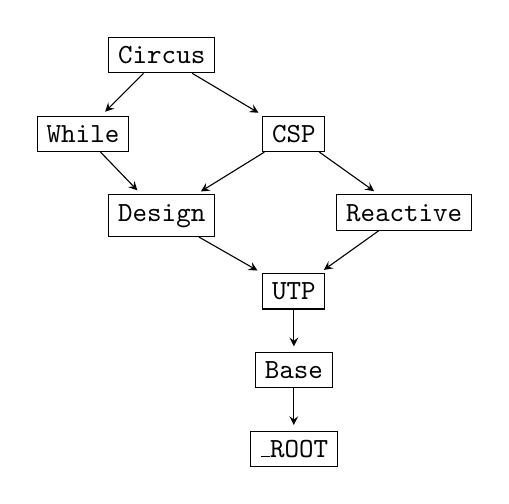
\begin{tikzpicture}[>=stealth,->,shorten >=2pt,looseness=.5,auto]
     \matrix[matrix of nodes,
             nodes={rectangle,draw,minimum size=4mm},
             column sep={1cm,between origins},
             row sep={1cm,between origins}]
      {              & |(X)|\texttt{Circus}  \\
        |(W)|\texttt{While} &              & |(C)|\texttt{CSP}                 \\
                     & |(D)|\texttt{Design} &              & |(R)|\texttt{Reactive}  \\
                     &              & |(u)|\texttt{UTP}              \\
                     &              & |(b)|\texttt{Base}                   \\
                     &              & |(r)|\texttt{\_ROOT}                 \\
      };
      \draw(X) -- (W) ; \draw (X) -- (C) ;
      \draw(W) -- (D) ; \draw (C) -- (D) ; \draw (C) -- (R) ;
      \draw (D) -- (u) ; \draw (R) -- (u) ;
      \draw (u) -- (b) ;
      \draw (b) -- (r) ;
    \end{tikzpicture}
  \caption{A Hierarchy of \texttt{Theory}s}
  \label{fig:hier-of-theory}
\end{figure}
Here we see theory slices organised as an acyclic directed graph,
where each slice inherits material from those below it.
At the bottom we have the \texttt{\_ROOT Theory} (slice),
which is hardwired in%
\footnote{
\texttt{\_ROOT} is the only thing hardwired---all other slices and their hierarchy
can be custom-built to suit the user.
}%
, and simply contains just the axioms of the underlying logic.

When we start a proof of a conjecture,
we do so from a given theory slice.
Imagine as an example, we state the following conjecture as part of theory \texttt{While}
(a simple imperative language):
\[
  \LNAME{$:=$-self-seq}
  \quad
  ( x:= e \comp x := f) =  x := f[e/x]
\]
We then start operating in a \emph{Proof Context} that consists
of the sequence of theory slices from \texttt{While} down to\texttt{ \_ROOT}.
This defines all the information about laws, definitions, know observation variables
that are in scope at the point were the conjecture is defined.
A successful proof of such a conjecture will result in it being added
to the collection of laws associated with its theory,
namely \texttt{While} in this example.

Another important principle is that when matching part of the proof of
{\LNAME{$:=$-self-seq}}
against a law in the \texttt{UTP} theory (say), the proof context is
shrunk to that from \texttt{UTP} down.
This is to ensure that specific uses of a name in a higher theory
(e.g. $J$ in Design, as per {\LNAME{$J$-def}})
does not mask a possible general use of $J$ as a schematic variable
in a lower theory%
\footnote{Variable $J$ may not be a plausible general predicate variable,
but $B$ is, and yet it is given a specific definition in \texttt{Reactive}.}%
.

%\newpage
%\input{src/ProofReplay.lhs}
%\newpage
%\input{src/Synchronise.lhs}
%\newpage
%\input{src/Program.lhs}
%\newpage
%\input{src/Verification.lhs}

%\chapter{I/O Infrastructure}
%
%\newpage
%\input{src/Files.lhs}
%\newpage
%\input{src/ImportExport.lhs}
%\newpage
%\input{src/Archive.lhs}
%
%\newpage
%\input{src/DocTextParser.lhs}
%\newpage
%\section{\LaTeX\ Formatting}

In this section we describe the \LaTeX\ notation
used to input theory information into \Saoithin.
We base our description around the components of the \texttt{Theory}
(a.k.a. \texttt{ProofContext}) datatype.

\subsection{Theory-Related \LaTeX\ Environments}

Each major component of the ProofContext datatype
has its components described within
a specific \LaTeX\ environment,
which we list below.

\begin{description}
  \item[\texttt{ctxtName,ctxtSeqNo :: String,Int}]~\\
    We use a single macro within a \texttt{theoryid} environment
    to encode these two values:
    \begin{verbatim}
    \begin{theoryid}
    \theoryNameVersion{LaTeX-Test}{99}
    \end{theoryid}
    \end{verbatim}
  \item[\texttt{typedefs :: Trie Type}]~\\
    Type-definition maps a (type-)name to a type(-definition).
    \\\verb"\begin{typedef}"
    \\ \phantom{mm}\textit{\textsf{name1}} \verb" & \defs & "\textit{\textsf{type1}}
    \\ \verb"\\" \textit{\textsf{  name2}} \verb" & \defs & "\textit{\textsf{type2}}
    \\ \ldots
    \\\verb"\end{typedef}"
    \\ An issue that arises is how the parser distinguishes between
    a newline (double-backslash) acting as a definition separator
    from one acting to split a long righthand-side over multiples lines (e.g.):
    \\ \phantom{mm}\textit{\textsf{name1}} \verb" & \defs & "\textit{\textsf{a-long}}
    \\ \verb"\\        &       & "\textit{\textsf{type-expression}}
    \\ \verb"\\" \textit{\textsf{  name2}} \verb" & \defs & "\textit{\textsf{type2}}
    \\ Perhaps we need an explixit \LaTeX\ macro (\verb"\next" ?)
    to denote definition separation?
  \item[\texttt{consts :: Trie Expr}]~\\
    Constant-definition maps a (variable-)name to a ground expr(-definition).
    \\\verb"\begin{consts}"
    \\ \phantom{mm}\textit{\textsf{name}} \verb" & \defs & "\textit{\textsf{expr}}
    \\\verb"\end{consts}"
        \\(From here on, we only list a single element).
  \item[\texttt{exprs :: Trie Expr}]~\\
    Expression-definition maps a (expr-)name to a expr(-definition).
    \\\verb"\begin{exprs}"
    \\ \phantom{mm}\textit{\textsf{name}} \verb" & \defs & "\textit{\textsf{expr}}
    \\\verb"\end{exprs}"
  \item[\texttt{preds :: Trie Pred}]~\\
    Predicate-definition maps a (expr-)name to a predicate(-definition).
    \\\verb"\begin{preds}"
    \\ \phantom{mm}\textit{\textsf{name}} \verb" & \defs & "\textit{\textsf{pred}}
    \\\verb"\end{preds}"
  \item[\texttt{obs :: Trie Type}]~\\
    Observation table maps a (variable-)name to a type.
    \\\verb"\begin{obs}"
    \\ \phantom{mm}\textit{\textsf{name}} \verb" & : & "\textit{\textsf{type}}
    \\\verb"\end{obs}"
  \item[\texttt{precs :: Trie Precs}]~\\
    Precedences table maps a (operator-)name to precedence data.
    \\\verb"\begin{precs}"
    \\ \phantom{mm}\textit{\textsf{name}} \verb" & \defs & "\textit{\textsf{prec}}
    \\\verb"\end{precs}"
  \item[\texttt{types :: Trie Type}]~\\
    Type table maps a (variable-)name to its type.
    \\\verb"\begin{types}"
    \\ \phantom{mm}\textit{\textsf{name}} \verb" & : & "\textit{\textsf{type}}
    \\\verb"\end{types}"
  \item[\texttt{alphas :: Trie Alphabet}]~\\
    Alphabet table maps a (predicate-)name to its alphabet.
    \\\verb"\begin{alphas}"
    \\ \phantom{mm}\textit{\textsf{name}} \verb" & \hasalpha??? & "\textit{\textsf{alpha}}
    \\\verb"\end{alphas}"
  \item[\texttt{laws :: LawTable}]~\\
    Law table maps a (law-)name to laws
    \\\verb"\begin{laws}"
    \\ \phantom{mn}\textit{\textsf{name}} \verb" & \defs & "\textit{\textsf{law}}  (axiom)
    \\ \verb"\\"   \textit{\textsf{name}} \verb" &   =   & "\textit{\textsf{law}}  (theorem)
    \\\verb"\end{laws}"
  \item[\texttt{conjectures :: Trie Law}]~\\
    Conjecture table maps a (conjecture-)name to laws
    \\\verb"\begin{conjectures}"
    \\ \phantom{mm}\textit{\textsf{name}} \verb" & \defs & "\textit{\textsf{law}}
    \\\verb"\end{conjectures}"
  \item[\texttt{theorems :: Trie Proof}]~\\
    Conjecture table maps a (proof-)name to proof
    \\\verb"\begin{theorems}"
    \\ \phantom{mm}\textit{\textsf{name}} \verb" & \hasproof??? & "\textit{\textsf{proof}}
    \\\verb"\end{theorems}"
\end{description}

\newpage
\subsection{The \LaTeX\ Syntax of Types}

\begin{verbatim}
B                                \bool
Z                                \num
Tprod [Type]                     ... \cross ...
Tfun Type Type                   ... \fun  ...
Tpfun Type Type                  ... \pfun ...
Tmap Type Type                   ... \ffun ...
Tset Type                        \power ...
Tseq Type                        \seq ...
Tseqp Type                       \seq_1 ...
Tfree String [(String,[Type])]    ...  ::=  (... \ldata ... \rdata ) * |
Tvar String                      ...
Tenv                             \Env
Terror String                    ...
Tarb                             \tarb
\end{verbatim}


\newpage
\subsection{The \LaTeX\ Syntax of Expressions}

\begin{verbatim}
T
F
Num Int
Var String
Prod [Expr]
App String Expr
Bin String Int Expr Expr
Equal Expr Expr
Set [Expr]
Setc QVars Pred Expr
Seq [Expr]
Seqc QVars Pred Expr
Map [(Expr,Expr)]
Cond Pred Expr Expr
Build String [Expr]
The QVars Pred Pred -- definite description
Evar String -- meta-variable denoting an expression
Eqvar String  -- meta-variable denoting a quantified variable
Eabs QVars Expr
Esub Expr ESubst
Eerror String
Efocus Expr [(Expr,Int)] -- focus, parent-list
\end{verbatim}


\newpage
\subsection{The \LaTeX\ Syntax of Predicates}

\begin{verbatim}
TRUE
FALSE
Obs Type Expr -- type is "underlying type" (See Types.lhs).
Defd Expr
TypeOf Expr Type
Not Pred
And [Pred]
Or [Pred]
Imp Pred Pred
Eqv Pred Pred
Forall QVars Pred Pred
Exists QVars Pred Pred
Exists1 QVars Pred Pred
Univ Pred
Sub Pred ESubst
Pvar String -- predicate meta-variable
>  -- UTP fundamentals
If Pred Pred Pred
Comp Pred Pred
NDC Pred Pred
RfdBy Pred Pred
LPredPred String Int Pred Pred -- e.g  Pre |- Post
LVarExpr String Int String Expr --  e.g.  x := e
LExprPred String Int Expr Pred  --  e.g.  c * P,  a --> P
LPredExprPred String Int Pred Expr Pred -- e.g   P [| S |] Q
Peabs String Pred  -- abstracting over an expression variable
Ppabs String Pred  -- abstracting over a predicate variable
Papp Pred Pred
Pfocus FContext Pred [(Pred,Int,FContext)] -- focus, ancestors
\end{verbatim}


\newpage
\subsection{The \LaTeX\ Syntax of Side-Conditions}

\begin{verbatim}
SCtrue
SCisCond String -- no dashed variables
SCnotFreeInP [String]  String -- Qvar, Pvar
SCnotFreeInE [String] String -- Qvar, Eevar
SCareTheFreeOfP [String] String -- Qvar, Pvar
SCcoverTheFreeOfP [String] String -- Qvar, Pvar
SCAnd [SideCond]
\end{verbatim}


%\newpage
%\input{src/LaTeXNames.lhs}
%\newpage
%\input{src/LaTeXSetup.lhs}
%\newpage
%\input{src/LaTeXPretty.lhs}
%\newpage
%\input{src/LaTeXTest.lhs}

%\chapter{Theories}
%
%\newpage
%\input{src/RootTheory.lhs}
%\newpage
%\section{Logic}\label{sec:logic}

The logic of \UTP2\ is an adaptation of the first-order equational logic
described by Tourlakis \cite{journals/logcom/Tourlakis01},
that fully formalises the logic of Dijkstra, Gries and Schneider \cite{gries.93}.
For this paper, we simply present the syntax and axioms of
a small first-order subset of
the whole logic,
sufficient to motivate and explain the required behaviour of the matcher.

We define our logic syntax
over a collection of given sets characterising different name-spaces:
\RLEQNS{
   x,y,z \in Var && (given) & \mbox{Variables}
\\ k \in Const && (given) & \mbox{Constants}
\\ f,g,h \in Name && (given) & \mbox{(Function) Names}
\\ E,F,G \in EName && (given) & \mbox{Expression Metavariable Names}
\\ P,Q,R \in PName && (given) & \mbox{Predicate Metavariable Names}
}
Constants and function names are as one would expect
in a logic with associated equational theories,
but we also have explicit meta-variables%
\footnote{Cover the role of ``schematic'' variables in some other logic presentations}
 for expressions
and predicates, in the object logic, as many UTP laws
are expressed using such.
Variables need special treatment, discussed further in Sec. \ref{sec:variables}.

Expressions denote values in the ``world of discourse'' (observations)
and are implicitly typed:
\RLEQNS{
   b,e \in Expr &::=& k | x  & \mbox{Expressions}
\\              &|& f~e & \mbox{Applications}
\\              &|& E & \mbox{Explicit Metavariable}
\\              &|& e[ e/x ] & \mbox{Explicit Obs. Substitution}
}
Expressions whose type is boolean ($b \in Expr$)
form the class
of \emph{atomic predicates}.
Predicates are defined much as expected:
\RLEQNS{
   p,q,r \in Pred &::=& \False & \mbox{Constant Predicates}
\\              &|& b & \mbox{Atomic Predicate}
\\              &|& p~ \lor q & \mbox{Disjunction}
\\              &|& P & \mbox{Explicit Metavariable}
\\              &|& \forall x,\ldots,x @ p & \mbox{Universal Quantifier}
\\              &|& p[ e,\ldots,e/x,\ldots,x ] & \mbox{Explicit Obs. Substitution}
}
One point to note is that the syntax includes explicit substitutions,
as these feature prominently in many UTP theories
(e.g. laws regarding assignment and sequential composition,
of the reactive healthiness condition \RR2).

We define a Law to be a pair,
consisting of a predicate and an associated side-condition ($Side$).
Side-conditions are a conjunction of zero or more basic conditions,
which typically capture relationships between given variables and
the free variables ($\fv$) of given predicates or expressions.
\begin{eqnarray*}
   sc \in Side &::=&  x \notin \fv.P
         | \setof{x,y,\ldots} = \fv.P
         | \setof{x,y,\ldots} \supseteq \fv.P
\\ Law &=& Pred \times Side
\end{eqnarray*}

%\newpage
%\input{src/GSLogic.lhs}
%\newpage
%\input{src/GS3001.lhs}
%\newpage
%\input{src/Builtin.lhs}
%\newpage
%\section{UTP}\label{sec:utp}

\PLAN{ Describing the more ubiquitous operators of UTP,
and why we want to handle alphabets implicitly.}

Some key concepts are common to most UTP theories,
namely sequential composition ($\comp$), non-deterministic choice ($\sqcap$),
refinement ($\refinedby$) and conditional ($\cond c$).
Importantly, in most theories these all have the same definition:
\begin{eqnarray*}
% \nonumber to remove numbering (before each equation)
  P \comp Q &\defs& \exists Obs_m @ P[Obs_m/Obs'] \land Q[Obs_m/Obs] \\
  P \sqcap Q &\defs& P \lor Q \\
  P \refinedby Q &\defs& [ Q \implies P ] \\
  P \cond c Q &\defs& c \land P \lor \lnot c \land Q
\end{eqnarray*}
The definitions for $\sqcap$, $\refinedby$ and $\cond c$ are unproblematical,
and are easily handled by the existing machinery,
with one key extension.
The definition of $\comp$ not only makes use of explicit substitution notation,
but also raises the question of how to interpret $Obs_m$, $Obs'$ and $Obs$.
Clearly they stand for the obervational variables of a UTP theory along with
appropriate decorations, but how do we support this?
In particular, how can we arrange matters so that
we only define $\comp$ once, in such a way that it can be used by many different theories?
We will first address the key extension alluded to above,
and then return to the problem of sequential composition.

\subsection{Defining your own language in \UTP2}

A key aspect of a UTP theory is the signature that captures the
abstract syntax of the language being defined.
This means that \UTP2\ needs to support user-defined languages.
This is achieved by having a table-driven parser for entering predicates,
and providing a facility for the user to add new entries
to the relevant tables:
\begin{eqnarray*}
Theory &=& \textbf{record} \ldots
\\ && precs : Name \pfun Precedence
\\ && lang : Name \pfun LangSpec
\\ && \ldots \textbf{end}
\end{eqnarray*}
The $precs$ table maps the name of an infix operator
to information about its parsing precedence and its associativity.
The $lang$ table maps a language construct name to a language specification
($LangSpec$) that describes the concrete syntactical structure of that construct.
A language specification is a mix of keywords denoting syntactical components
like variables (V) , expressions (E) , predicates (P),
 or various lists of such,
interspersed with concrete syntax symbols.
We won't give a full definition here but present some examples to give the
idea:
\begin{itemize}
  \item
    Refinement: we specify this as ``\verb@P |= P@'',
  which states that \verb@|=@ is an infix operator between two predicates.
  When this is entered into the $lang$ table,
  a corresponding entry is automatically created in the $precs$
  table with default values (mid-range precedence, non-associative)
  which can then be edited by the user to suit.
  Also entered is a dummy definition for the construct
  into the $laws$ table, which itself then needs to be edited.
  \item Assignment:
    specified as ``\verb@V := E@'', stating that \verb@:=@
    is an infix operator in-between a variable and expression,
    resulting in a predicate.
\end{itemize}
In general defining a language construct (resulting in a predicate)
 involves adding entries
to the $lang$ and $laws$ tables,
and possibly also to the $types$ and $precs$ tables, depending
on the precise nature of the construct.
Infix expression operators do not have $lang$ entries
but require $laws$, $precs$ and $types$ entries.

When we talk about developing a theory of Designs (Section \ref{sec:designs}),
we shall give a worked-out example of  a language definition.

\subsection{The problem with $\protect\comp$}

The definition of sequential composition,
\begin{eqnarray*}
P \comp Q &\defs& \exists Obs_m @ P[Obs_m/Obs'] \land Q[Obs_m/Obs]
\end{eqnarray*}
says in effect that for each observation, $x$, say, in $Obs$,
we replace any free occurrence of $x'$ in $p$ by $x_m$
and any free occurrence of $x$ in $q$ by $Obs_m$,
and use existential quantification to hide $x_m$.
In effect the rule above is really a rule-schema,
characterising an infinite number of rules,
one for each possible alphabet represented by $Obs$.
However, we don't want to repeatedly instantiate this rule
and reason about its consequences for each specific alphabet we use.
In fact, we want to use the definition in cases where only part
of the alphabet is known (Designs again, Section \ref{sec:designs}).
We would prefer to be able to do proofs with the definition
as given above, only instantiating $Obs$ where necessary,
and then perhaps only partially.
In fact, we want to support the following proof
(of the associativity of $\comp$)
which does not require any instantation of $Obs$:
{\small
\begin{eqnarray*}
  && P ; (Q ; R)
\\&\equiv& \exists Obs_m @ P[Obs_m/Obs']
           \land (Q;R)[Obs_m/Obs]
\\&\equiv& \exists Obs_m @ P[Obs_m/Obs']
           \land (\exists Obs_n @ Q[Obs_n/Obs'] \land R[Obs_n/Obs])[Obs_m/Obs]
\\&\equiv& \exists Obs_m,Obs_n @ P[Obs_m/Obs']
           \land Q[Obs_n/Obs'][Obs_m/Obs]
           \land R[Obs_n/Obs][Obs_m/Obs]
\\&\equiv& \exists Obs_m,Obs_n @
                  P[Obs_m/Obs'][Obs_n/Obs']
           \land Q[Obs_n,Obs_m/Obs',Obs]
           \land R[Obs_n/Obs]
\\&\equiv& \exists Obs_n @
                  (\exists Obs_m @ P[Obs_m/Obs'][Obs_n/Obs']
           \land Q[Obs_m/Obs][Obs_n/Obs'])
\\&& \qquad\qquad {} \land R[Obs_n/Obs]
\\&\equiv& \exists Obs_n @
                  (\exists Obs_m @ P[Obs_m/Obs']
           \land Q[Obs_m/Obs])[Obs_n/Obs']
           \land R[Obs_n/Obs]
\\&\equiv& \exists Obs_n @
                  (P ; Q)[Obs_n/Obs']
           \land R[Obs_n/Obs]
\\&\equiv&(P ; Q) ; R
\end{eqnarray*}
}
In effect we want to reason within our logic about ``schematic''
variables like $Obs$ and treat the substitution notation as part
of the object logic, rather than meta-notation describing
the behaviour of an inference rule.

To achieve this we have to add another linguistic innovation
to the logic.
A common shorthand in most presentations of logic is to
view $\forall x,y,z @ p$ (say)
as a shorthand for $\forall x @ \forall y @ \forall z @ p$.
Our innovation is not only to add the former as a full part
of the logic syntax, but also a further extension.
We want to be able to have quantifier variables (e.g. $Obs$)
that represent lists of ``ordinary'' quantifier variables.
We do this by splitting the list into two parts, separated by
a semi-colon, with those in the first part being ordinary,
whilst those in the second part denote lists of variables.
The revised syntax of $\forall$ is now:
$$
\forall x_1,\ldots,x_m \qsep xs_1, \ldots , xs_m @P
\qquad
m \geq 0, n \geq 0, m+n \geq 1
$$
Other observation (1st-order) quantifiers are modified similarly.
The $x_i$ and $xs_j$ above are ``quantifier variables'',
and will be disambiguated were necessary by referring to the $x_i$
(before the $\qsep$ sysmbol) as ``single variables''
and the $xs_j$ (after $\qsep$ as ``list variables'').
A list where $m=0$ is referred to as an ``ordinary list''.
The meaning of a quantifier variable list of the
form $x_1,\ldots,x_m \qsep xs_1, \ldots , xs_m$
is that it matches an ordinary list
of the form $y_1,\ldots,y_{m+k}, k \geq 0$
where each $x_i$ binds to one $y_j$,
each $xs_i$ binds to zero or more $y_j$,
and every $y_j$ is bound exactly once.
In principle the bindings associated with a variable like $xs_i$
are non-deterministic, albeit they must be consistent with bindings derived
from the match as a whole, i.e. the wider context in which that  variable occurs.
In practice, heuristics are used in the implementation to select
a binding that is hopefully as ``good'' as possible.

As our proof above largely depended on properties of (explicit)
substitution, we have to add it into our logic as well.
So we revise our syntax for predicates:
\RLEQNS{
   p,q,r \in Pred &::=& \ldots
\\              &|& \yen qvs @ p & \mbox{1st-order Quantifiers, } \yen \in \setof{\forall,\exists,\exists!}
\\              &|& p[ e/x ] & \mbox{Explicit Obs. Substitution}
\\              &|& p[ e/E ] & \mbox{Explicit E-var. Substitution}
\\              &|& p[ p/P ] & \mbox{Explicit P-var. Substitution}
\\ qvs \in QVars &&& \mbox{Quantifier Variable lists}
\\ &::=~& x_1,\ldots,x_m \qsep xs_1, \ldots , xs_m
   & m \geq 0, n \geq 0, m+n \geq 1
}
Explicit substitutions are also added to expressions as well.
Laws regarding explicit substitutions also need to be developed,
e.g.
$$
p[e/x][f/y] = p[e,f/x,y], \quad x \neq y, y \notin \fv.e
$$
but we do not list these here.

This extension allows us to introduce axioms like:
$$
\AXallOInst \qquad \AXallOInstN
$$
rather than relying on a simple single quantifier axiom
and the usual conventions regarding the $\forall x,y,z$ shorthand.
In essence what we have done is to formalise and automate this convention.

To support the definition of $\comp$ we need one further step.
The list variable $Obs$ does not stand for an arbitrary
list of single variables, but is instead intended to stand for
precisely those un-dashed variables that are present in the
alphabet of the current theory, even if that alphabet
has not been fully described.
Similarly, $Obs'$ stands for all the dashed variables,
and $Obs_m$ denotes the decoration of all the $Obs$ variables.
In effect we designate certain list variables (like $Obs$)
as having a special meaning.

The basic matcher described in Section \ref{sec:logic},
has to be enhanced to perform appropriate matching
where non-ordinary quantifier lists are present.
To make this work, we need to extend theories to have
a table that records the theory alphabet:
\begin{eqnarray*}
Theory &=& \textbf{record} \ldots
\\ && obs : Name \pfun Type
\\ && \ldots \textbf{end}
\end{eqnarray*}
The $obs$ table needs to become part of the matching context $\Gamma$,
and we introduce rules for matching quantifier lists:
\begin{eqnarray*}
  & \inferrule%
       {~}%
       {\Gamma \vdash \qsep Obs \ddagger \qsep Obs | \varepsilon }
\\
\\& \inferrule%
       {Obs(\Gamma)=\setof{o_1,\ldots,o_n}}%
       {\Gamma \vdash \qsep Obs \ddagger \setof{o_1,\ldots,o_n}
         | \setof{Obs \mapsto \setof{o_1,\ldots,o_n}}}
\end{eqnarray*}
The first rule allows $Obs$ to match itself, and so we can do proofs
that do not require it to be expanded to an ordinary list.
Note also that in this case an empty binding ($\varepsilon$) is returned.
Other matching rules not shown here, take care of decorations,
ensuring that $Obs$ matches $x,y,z$, if appropriate,
but not $x',y',z'$.

We can now define sequential composition in our revised logic as:
\begin{eqnarray*}
P \comp Q &\defs& \exists \qsep Obs_m @ P[Obs_m/Obs'] \land Q[Obs_m/Obs]
\end{eqnarray*}
and produce a proof as shown earlier.
There is an additional extension required to the logic to do this,
but we shall motivate and introduce it
in the section on Designs (Section \ref{sec:designs}).

%\newpage
%\input{src/RAlg.lhs}
%\newpage
%\input{src/R.lhs}
%\newpage
%\input{src/Design.lhs}
%
%\chapter{Tests}
%
%\newpage
%\input{src/TestFramework.lhs}
%\newpage
%\input{src/AdHocTests.lhs}

\chapter{wxWidgets User Interface}

\newpage
\input{src/WxTypes.lhs}
\newpage
\input{src/WxState.lhs}
%\newpage
%\input{src/WxFiles.lhs}
%\newpage
%\input{src/WxStyle.lhs}
%\newpage
%\input{src/WxRenderOld.lhs}
%\newpage
%\input{src/WxRender.lhs}
%
\newpage
\input{src/WxProof.lhs}
%\newpage
%\input{src/WxTheory.lhs}
%\newpage
%\input{src/WxSynchro.lhs}
%\newpage
%\input{src/WxProg.lhs}%%


 MAINLINE
\newpage
\input{src/UTP2.lhs}

\newpage
\bibliography{doc/SAOITHIN}

%\appendix
%\chapter{Prototyping}

\newpage
\input{proto/ProtoFocus.lhs}
\newpage
\input{proto/ProtoFocus2.lhs}
\newpage
\input{proto/ProtoMatch.lhs}

\section{Displaying UTP2LogicDefs}


\verb"\DEFOEESUBST"
\DEFOEESUBST

\newpage
\verb"$$\DEFOEPSUBST{xxx}$$"
$$\DEFOEPSUBST{xxx}$$


\verb"\DEFEEESUBST"
\DEFEEESUBST

\verb"\DEFPPESUBST"
\DEFPPESUBST


\newpage
\verb"$$\DEFEEPSUBST{xxx}$$"
$$\DEFEEPSUBST{xxx}$$


\newpage
\verb"$$\DEFPPPSUBST{xxx}$$"
$$\DEFPPPSUBST{xxx}$$

%\def\AXeqvAssocL{(P\equiv Q)\equiv R}
%\def\AXeqvAssocR{P\equiv (Q\equiv R)}
%\def\AXeqvAssoc{(\AXeqvAssocL) \equiv (\AXeqvAssocR)}
%\def\AXeqvAssocN{\LNAME{Ax-$\equiv$-assoc}}
%
%\def\AXeqvSymm{P\equiv Q\equiv Q \equiv P}
%\def\AXeqvSymmN{\LNAME{Ax-$\equiv$-symm}}
%
%\def\AXeqvId{\textit{true} \equiv Q\equiv Q}
%\def\AXeqvIdN{\LNAME{Ax-$\equiv$-id}}
%
%\def\AXfalseDef{\textit{false} \equiv \neg \mbox{\textit{true}}}
%\def\AXfalseDefN{\LNAME{Ax-$false$-def}}
%
%\def\AXnotEqvDistr{\neg(P\equiv Q) \equiv \neg P \equiv Q}
%\def\AXnotEqvDistrN{\LNAME{Ax-$\neg$-$\equiv$-distr}}
%
%\def\AXorSymm{P\vee Q \equiv  Q \vee P}
%\def\AXorSymmN{\LNAME{Ax-$\vee$-symm}}
%
%\def\AXorAssoc{(P\vee Q) \vee R \equiv  P \vee (Q \vee R)}
%\def\AXorAssocN{\LNAME{Ax-$\vee$-assoc}}
%
%\def\AXorIdem{P\vee P \equiv P}
%\def\AXorIdemN{\LNAME{Ax-$\vee$-idem}}
%
%\def\AXorEqvDistr{P \vee (Q\equiv R) \equiv P\vee Q \equiv P \vee R}
%\def\AXorEqvDistrN{\LNAME{Ax-$\vee$-$\equiv$-distr}}
%
%\def\AXexclMdl{P \vee \neg P}
%\def\AXexclMdlN{\LNAME{Ax-Excl-Mdl}}
%
%\def\AXgoldRule{P\wedge Q \equiv  P \equiv Q \equiv P \vee Q}
%\def\AXgoldRuleN{\LNAME{Ax-Golden-Rule}}
%
%\def\AXimplDef{P\Rightarrow Q \equiv P\vee  Q \equiv Q}
%\def\AXimplDefN{\LNAME{Ax-$\implies$-def}}

\newpage
\verb"$$\AXPROP$$"
$$\AXPROP$$

%\def\AXorAllOScopeL{p \lor (\forall \qsep xs,ys @ q)}
%\def\AXorAllOScopeR{\forall \qsep xs @ p \lor (\forall \qsep ys @ q)}
%\def\AXorAllOScopeS{xs \notin p}
%\def\AXorAllOScopeN{\LNAME{Ax-$\lor$-$\forall x$-scope}}
%\def\AXorAllOScope{\AXorAllOScopeL \equiv \AXorAllOScopeR, \quad \AXorAllOScopeS}
%
%\def\AXorAllEScopeL{p \lor (\forall \qsep Es, Fs @ q)}
%\def\AXorAllEScopeR{\forall \qsep Es @ p \lor (\forall \qsep Fs @ q)}
%\def\AXorAllEScopeS{Es \notin p}
%\def\AXorAllEScopeN{\LNAME{Ax-$\lor$-$\forall E$-scope}}
%\def\AXorAllEScope{\AXorAllEScopeL \equiv \AXorAllEScopeR, \quad \AXorAllEScopeS}
%
%\def\AXorAllPScopeL{p \lor (\forall \qsep Ps,  Qs @ q)}
%\def\AXorAllPScopeR{\forall \qsep Ps @ p \lor (\forall \qsep Qs @ q)}
%\def\AXorAllPScopeS{ Ps \notin p}
%\def\AXorAllPScopeN{\LNAME{Ax-$\lor$-$\forall P$-scope}}
%\def\AXorAllPScope{\AXorAllPScopeL \equiv \AXorAllPScopeR, \quad \AXorAllPScopeS}
%
%\def\AXallODistrL{(\forall \qsep xs @ p \land q)}
%\def\AXallODistrR{(\forall \qsep xs @ p) \land (\forall \qsep xs @ q)}
%\def\AXallODistrN{\LNAME{Ax-$\forall x$-distr}}
%\def\AXallODistr{\AXallODistrL \equiv \AXallODistrR}
%
%\def\AXallEDistrL{(\forall \qsep Es @ p \land q)}
%\def\AXallEDistrR{(\forall \qsep Es @ p) \land (\forall \qsep Es @ q)}
%\def\AXallEDistrN{\LNAME{Ax-$\forall E$-distr}}
%\def\AXallEDistr{\AXallEDistrL \equiv \AXallEDistrR}
%
%\def\AXallPDistrL{(\forall \qsep Ps @ p \land q)}
%\def\AXallPDistrR{(\forall \qsep Ps @ p) \land (\forall \qsep Ps @ q)}
%\def\AXallPDistrN{\LNAME{Ax-$\forall P$-distr}}
%\def\AXallPDistr{\AXallPDistrL \equiv \AXallPDistrR}
%
%\def\AXallOInstL{\forall x\qsep xs @ p}
%\def\AXallOInstR{\forall \qsep xs  @ p[e/x]}
%\def\AXallOInstN{\LNAME{Ax-$\forall x$-inst}}
%\def\AXallOInst{(\AXallOInstL) \implies (\AXallOInstR)}
%
%\def\AXallEInstL{\forall E \qsep Es @ p}
%\def\AXallEInstR{\forall \qsep Es @ p[e/E]}
%\def\AXallEInstN{\LNAME{Ax-$\forall E$-inst}}
%\def\AXallEInst{(\AXallEInstL) \implies (\AXallEInstR)}
%
%\def\AXallPInstL{\forall P\qsep Ps @ p}
%\def\AXallPInstR{\forall \qsep Ps @ p[q/P]}
%\def\AXallPInstN{\LNAME{Ax-$\forall P$-inst}}
%\def\AXallPInst{(\AXallPInstL) \implies (\AXallPInstR)}
%
%\def\AXallORngL{\forall \qsep xs | r @ p}
%\def\AXallORngR{\forall \qsep xs @ r \implies p}
%\def\AXallORngN{\LNAME{Ax-$\forall x$-range}}
%\def\AXallORng{(\AXallORngL) \equiv (\AXallORngR)}
%
%\def\AXanyODefL{\exists \qsep xs @ p}
%\def\AXanyODefR{\lnot (\forall \qsep xs @ \lnot p)}
%\def\AXanyODefN{\LNAME{Ax-$\exists x$-def}}
%\def\AXanyODef{(\AXanyODefL) \equiv \AXanyODefR}
%
%\def\AXanyEDefL{\exists \qsep Es @ p}
%\def\AXanyEDefR{\lnot (\forall \qsep Es @ \lnot p)}
%\def\AXanyEDefN{\LNAME{Ax-$\exists E$-def}}
%\def\AXanyEDef{(\AXanyEDefL) \equiv \AXanyEDefR}
%
%\def\AXanyPDefL{\exists \qsep Ps @ p}
%\def\AXanyPDefR{\lnot (\forall \qsep Ps @ \lnot p)}
%\def\AXanyPDefN{\LNAME{Ax-$\exists P$-def}}
%\def\AXanyPDef{(\AXanyPDefL) \equiv \AXanyPDefR}
%
%\def\AXanyORngL{\exists \qsep xs | r @ p}
%\def\AXanyORngR{\exists \qsep xs @ r \land p}
%\def\AXanyORngN{\LNAME{Ax-$\exists x$-range}}
%\def\AXanyORng{(\AXanyORngL) \equiv (\AXanyORngR)}
%
%\def\AXoneODefL{\exists! \qsep xs @ p}
%\def\AXoneODefR{(\exists \qsep xs @ p)
%                 \land
%                 \exists \qsep ys @ p[ys/\qsep xs] \implies ys = xs}
%\def\AXoneODefN{\LNAME{Ax-$\exists! x$-def}}
%\def\AXoneODef{(\AXoneODefL) \equiv (\AXoneODefR)}
%
%\def\AXoneORngL{\exists! \qsep xs | r @ p}
%\def\AXoneORngR{\exists! \qsep xs @ r \land p}
%\def\AXoneORngN{\LNAME{Ax-$\exists! x$-range}}
%\def\AXoneORng{(\AXoneORngL) \equiv (\AXoneORngR)}
%
%\def\AXeqReflL{e}
%\def\AXeqReflR{e}
%\def\AXeqReflN{\LNAME{Ax-$=$-refl}}
%\def\AXeqRefl{\AXeqReflL = \AXeqReflR}
%
%\def\AXtheDefL{e=\theta x @ p}
%\def\AXtheDefR{p[e/x] \land (\forall y @ p[y/x] \implies y=e)}
%\def\AXtheDefS{x \notin e}
%\def\AXtheDefN{\LNAME{Ax-$\theta$-Def}}
%\def\AXtheDef{(\AXtheDefL) \equiv \AXtheDefR, \quad \AXtheDefS}
%
%\def\AXtheRngL{\theta x | r @ p}
%\def\AXtheRngR{\theta x @ r \land p}
%\def\AXtheRngN{\LNAME{Ax-$\theta$-range}}
%\def\AXtheRng{(\AXtheRngL) = (\AXtheRngR)}
%
%\def\AXObetaRedL{(\lambda x\qsep xs @ e)f}
%\def\AXObetaRedR{(\lambda \qsep xs @ e)[f/x]}
%\def\AXObetaRedN{\LNAME{Ax-$\beta$-OReduce}}
%\def\AXObetaRed{\AXObetaRedL = \AXObetaRedR}
%
%\def\AXEbetaRedL{(\Lambda E\qsep Es @ q)e}
%\def\AXEbetaRedR{(\Lambda \qsep Es @ q)[e/E]}
%\def\AXEbetaRedN{\LNAME{Ax-$\beta$-EReduce}}
%\def\AXEbetaRed{\AXEbetaRedL \equiv \AXEbetaRedR}
%
%\def\AXPbetaRedL{(\Lambda P\qsep Ps @ q)r}
%\def\AXPbetaRedR{(\Lambda \qsep Ps @ q)[r/P]}
%\def\AXPbetaRedN{\LNAME{Ax-$\beta$-PReduce}}
%\def\AXPbetaRed{\AXPbetaRedL \equiv \AXPbetaRedR}
%
%\def\AXLeibnizL{\bigwedge_{i=1}^n x_i = e_i}
%\def\AXLeibnizR{p \equiv p[\vec e/\vec x]}
%\def\AXLeibnizS{x_i \mbox{ distinct}}
%\def\AXLeibnizN{\LNAME{Ax-Leibniz}}
%\def\AXLeibniz{(\AXLeibnizL) \implies (\AXLeibnizR), \quad \AXLeibnizS}
%
%\def\AXOSubstR{p[\vec e/\vec x]}
%\def\AXOSubstL{p[\vec x:=\vec e]}
%\def\AXOSubstN{\LNAME{Ax-OSubst}}
%\def\AXOSubst{\AXOSubstL \equiv \AXOSubstR}
%
%\def\AXESubstL{p[\vec e/Es]}
%\def\AXESubstR{p[Es:=\vec e]}
%\def\AXESubstN{\LNAME{Ax-ESubst}}
%\def\AXESubst{\AXESubstL \equiv \AXESubstR}
%
%\def\AXPSubstL{p[\vec q/ Ps]}
%\def\AXPSubstR{p[ Ps:=\vec q]}
%\def\AXPSubstN{\LNAME{Ax-PSubst}}
%\def\AXPSubst{\AXPSubstL \equiv \AXPSubstR}
%
%\def\AXTrueOSubL{true[\vec e/ \vec x]}
%\def\AXTrueOSubR{true}
%\def\AXTrueOSubN{\LNAME{Ax-$true$-OSubst}}
%\def\AXTrueOSub{\AXTrueOSubL \equiv \AXTrueOSubR}
%
%\def\AXTrueESubL{true[\vec e/ Es]}
%\def\AXTrueESubR{true}
%\def\AXTrueESubN{\LNAME{Ax-$true$-ESubst}}
%\def\AXTrueESub{\AXTrueESubL \equiv \AXTrueESubR}
%
%\def\AXTruePSubL{true[\vec q/ Ps]}
%\def\AXTruePSubR{true}
%\def\AXTruePSubN{\LNAME{Ax-$true$-PSubst}}
%\def\AXTruePSub{\AXTruePSubL \equiv \AXTruePSubR}
%
%\def\AXFalseOSubL{false[\vec e/ \vec x]}
%\def\AXFalseOSubR{false}
%\def\AXFalseOSubN{\LNAME{Ax-$false$-OSubst}}
%\def\AXFalseOSub{\AXFalseOSubL \equiv \AXFalseOSubR}
%
%\def\AXFalseESubL{false[\vec e/ Es]}
%\def\AXFalseESubR{false}
%\def\AXFalseESubN{\LNAME{Ax-$false$-ESubst}}
%\def\AXFalseESub{\AXFalseESubL \equiv \AXFalseESubR}
%
%\def\AXFalsePSubL{false[\vec q/ Ps]}
%\def\AXFalsePSubR{false}
%\def\AXFalsePSubN{\LNAME{Ax-$false$-PSubst}}
%\def\AXFalsePSub{\AXFalsePSubL \equiv \AXFalsePSubR}

\newpage
\verb"$$\AXNONPROP$$"
$$\AXNONPROP$$


\newpage
\verb"$$\INFERENCES$$"
$$\INFERENCES$$

\verb"$$\DEDUCTION$$"
$$\DEDUCTION$$

\newpage
\verb"$$\DERIVED$$"
$$\DERIVED$$


\newpage
\section{Displaying UTP2FreeVarDefs}


\newpage
\input{src/TEMPLATES.lhs}

\newpage
\input{proto/ProtoMatchTypes-only.lhs}
\newpage
\input{src/MatchTypes-only.lhs}


\end{document}
